% Task C13
% Source volume: lower
% Physical scan pages: 13--51
% Printed book pages: 1--39
% Transcribe only source content; omit running headers, footers, and printed page numbers.
\chapter{数项级数}

本章是无穷级数理论的第一章。在 §13.1 中从无限项求和、部分和数列与广义积分三个角度对无穷级数的基本概念作综述。在 §13.2 和 §13.3 中讲述正项级数和一般项级数的判别法与性质。§13.4 用于介绍无穷乘积。最后一节是学习要点和两组参考题。（有关级数求和的问题将在 §16.2 集中讨论。）

\section{无限级数的基本概念}

\subsection{无限级数的多种视角}

可以从几个不同角度来理解无穷级数的概念。

首先，无穷级数是有限项求和的直接推广。下面是数学发展史上的几个重要例子，其中都涉及无穷级数问题（参见 [30, 56]）。

\begin{xexample}[13.1.1]
我国古代重要典籍《庄子》（约公元前 300 年）一书中有“一尺之棰，日取其半，万世不竭”。从数学上看，这与下列无穷项求和有密切联系：
\[
1=\frac12+\frac14+\frac18+\cdots+\frac1{2^n}+\cdots.
\]
\end{xexample}

\begin{xexample}[13.1.2]
古希腊伊利亚学派的 Zeno（芝诺）提出过 4 个著名的悖论，其中的 Achilles\footnote{Achilles（阿基里斯）是荷马史诗《伊利亚特》中的希腊名将，以快跑著称，被称为 The great runner。用无穷级数工具来解决 Zeno 悖论的想法最早来自 Gregory（格雷戈里，1647）。}悖论是：Achilles 永远追不上在他前面的一只乌龟，因为 Achilles 必须首先跑到乌龟的出发点，而在这段时间中乌龟又已经向前爬过一段距离，因此仍然在 Achilles 的前面，这种情况会无休止地继续下去。

若将上面提到的时间记为 $t_1$，并继续下去，问题就变成了计算 $t_1+t_2+\cdots$ 的和。这是一个无穷级数求和问题。虽然谁都知道 Achilles 一定会赶上乌龟，而且不难直接计算出所需要的时间，但是为了驳倒 Zeno 的说法，就需要有关于无穷级数的概念和工具，这超出了当时希腊数学的水平（见下一小节的思考题 1）。
\end{xexample}

\begin{xexample}[13.1.3]
古希腊数学家 Archimedes 求得抛物线弓形的面积是同底同高的三角形面积乘以因子 $\frac43$。如图 13.1 所示，其中作出了经过点 $A,B,C$ 的抛物线弓形和对应的三角形。由于过抛物线上点 $A$ 的切线平行于直线段 $BC$，因此它们符合同底（$BC$）同高（$AD$）的条件。从该图中又可以看出在抛物线弓形中去掉上述三角形之后又得到两个较小的抛物线弓形，于是又可以继续作出与它们分别为同底同高的两个三角形。Archimedes 证明它们的面积之和是第一个三角形面积的 $\frac14$，而且这个过程可以无限继续，因此就出现了无穷级数的求和问题：
\begin{equation}
1+\frac14+\frac1{4^2}+\cdots+\frac1{4^n}+\cdots=\frac43.
\tag{13.1}
\end{equation}
由于当时没有无穷级数的概念和极限理论，Archimedes 在论证中只能使用 Eudoxus（欧多克索斯）的穷竭法（详见 [56] 中 2.3.2 小节的（三）和（四））。

\begin{center}
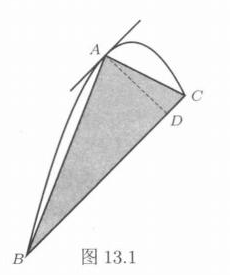
\includegraphics[width=.28\linewidth]{figures/lower/ch13/fig-13-1.png}
\end{center}
\end{xexample}

\begin{xexample}[13.1.4]
我国魏晋时代的数学家刘徽提出用“割圆术”来计算圆周率。他的方法是从计算圆的内接正六边形的面积出发，然后将内接正多边形的边数成倍增加，将每次增加的小三角形的面积累加，以得到越来越精确的圆面积值，从而求出圆周率 $\pi$ 的近似值。刘徽提出：“割之弥细，所失弥少，割之又割以至于不可割，则与圆合体而无所失矣。”这就是说圆面积是一个无穷级数之和（本题的分析将在本小节末完成）。
\end{xexample}

其次，对数列的研究就可引出无穷级数。在上册中我们已经有意识地这样做了。在 2.2.3 小节末的注解中（上册 24--25 页）引入了无穷级数
\begin{equation}
\sum_{n=1}^{\infty}a_n=a_1+a_2+\cdots+a_n+\cdots
\tag{13.2}
\end{equation}
的基本概念，其中包括通项 $a_n$，部分和数列 $S_n=a_1+a_2+\cdots+a_n$，$n=1,2,\ldots$。当部分和数列 $\{S_n\}$ 收敛时，称无穷级数 (13.2) 收敛，否则称 (13.2) 发散。当无穷级数 (13.2) 收敛时，称极限 $S=\lim_{n\to\infty}S_n$ 为无穷级数 (13.2) 的和，并记为
\[
\sum_{n=1}^{\infty}a_n=a_1+a_2+\cdots+a_n+\cdots=S.
\]
此外，对于 $S$ 为无穷大量，即部分和数列 $\{S_n\}$ 有广义极限的情况，也写为 $\sum_{n=1}^{\infty}a_n=S$。为简明起见，常将无穷级数简称为级数，有时还将 $\sum_{n=1}^{\infty}a_n$ 简记为 $\sum a_n$。

对收敛级数来说，还需要有余项概念。设 $\sum_{n=1}^{\infty}a_n$ 收敛，则级数 $\sum_{k=n+1}^{\infty}a_k$ 对每个 $n$ 均收敛。将它的和 $R_n$ 称为收敛级数 $\sum_{n=1}^{\infty}a_n$ 的第 $n$ 个余项。若将级数 $\sum_{n=1}^{\infty}a_n$ 的部分和数列记为 $\{S_n\}$，记级数的和为 $S$，则就有 $R_n=S-S_n$，因此作为数列的余项 $\{R_n\}$ 一定是无穷小量：$\lim_{n\to\infty}R_n=0$。

由级数的定义可见，从给定的数列 $\{a_n\}$ 出发可以构造一个级数
\begin{equation}
a_1+\sum_{n=1}^{\infty}(a_{n+1}-a_n),
\tag{13.3}
\end{equation}
使得两者同时收敛或发散。当它们收敛时，级数 (13.3) 的和 $S$ 就等于数列的极限：$\lim_{n\to\infty}a_n=S$。今后将会看到，对于给定的数列构造级数 (13.3) 是研究数列以及计算其极限的一种有用方法。

由于级数与数列的上述联系，关于级数的不少性质可以从数列的性质直接推出。首先是级数收敛的必要条件：
\begin{equation}
\sum_{n=1}^{\infty}a_n\ \text{收敛}\quad\Longrightarrow\quad \lim_{n\to\infty}a_n=0.
\tag{13.4}
\end{equation}
其证明见例题 2.2.9。同时在那里已经指出，这不是级数收敛的充分条件。

由数列的 Cauchy 收敛准则（见 §3.4）就得到级数的 \textbf{Cauchy 收敛准则}：级数 $\sum a_n$ 收敛的充分必要条件是对于每个 $\varepsilon>0$，存在正整数 $N$，使得对满足条件 $n>N$ 的正整数 $n$ 和每个正整数 $p$，成立不等式
\begin{equation}
\abs{a_{n+1}+a_{n+2}+\cdots+a_{n+p}}<\varepsilon.
\tag{13.5}
\end{equation}
注意：若于 (13.5) 中令 $p=1$，就得到收敛级数的必要条件 (13.4)。此外，上册中的例题 3.4.1 和 3.4.2 就是这个收敛准则在无穷级数上的应用。

若级数 $\sum a_n$ 的每一项同号，则称该级数为同号级数。习惯上称非负项级数为正项级数。显然对同号级数只需研究正项级数就够了。对于正项级数，其部分和数列为单调增加数列，因此就知道：\textbf{正项级数收敛的充分必要条件是其部分和数列有上界}。

在上册中已经介绍了几个重要的正项级数。例如，已经用多种方法证明调和级数 $\sum_{n=1}^{\infty}\frac1n$ 发散（见例题 2.2.6，3.4.2）。进一步是关于 $p$ 次幂的调和级数（简称为 $p$ 级数）$\sum_{n=1}^{\infty}\frac1{n^p}$ 的敛散性结论：当 $p\leq1$ 时发散，当 $p>1$ 时收敛（见 2.2.4 小节的题 9 和 2.3.2 小节的题 6）。在命题 2.5.2 中得到了自然对数的底 $\ee$ 的无穷级数表示，并将它用于 $\ee$ 的近似计算与无理性证明中。

对无穷级数的第三个视角是将它与上册第十二章的广义积分作比较。例如，在级数 $\sum_{n=1}^{\infty}a_n$ 与无穷限广义积分 $\int_a^{+\infty}f(x)\,\dd x$ 的基本概念之间，存在离散 $\leftrightarrow$ 连续的对应关系：$n\leftrightarrow x$，$a_n\leftrightarrow f(x)$，$S_n=\sum_{k=1}^{n}a_k\leftrightarrow\int_a^A f(x)\,\dd x$ 和 $R_n=\sum_{k=n+1}^{\infty}a_k\leftrightarrow\int_A^{+\infty}f(x)\,\dd x$。

在敛散性判别方面级数理论为广义积分提供了以下两个工具：

\begin{xproposition}[13.1.1]
设 $f$ 于 $[a,+\infty)$ 上内闭可积，则广义积分 $\int_a^{+\infty}f(x)\,\dd x$ 收敛的充分必要条件是：对于发散于正无穷大的每个数列 $\{A_n\}\subset[a,+\infty)$，级数
\[
\sum_{n=1}^{\infty}\int_{A_{n-1}}^{A_n}f(x)\,\dd x
\]
收敛，其中 $A_0=a$。
\end{xproposition}

\begin{xproposition}[13.1.2]
设 $f$ 于 $[a,+\infty)$ 上内闭可积且不变号，则 $\int_a^{+\infty}f(x)\,\dd x$ 收敛的充分必要条件是：存在发散于正无穷大的严格单调增加数列 $\{A_n\}\subset[a,+\infty)$，使同号级数
\[
\sum_{n=1}^{\infty}\int_{A_{n-1}}^{A_n}f(x)\,\dd x
\]
收敛，其中 $A_0=a$。
\end{xproposition}

\begin{xremark}
在例题 12.2.5 中实际上已经用了这个命题。又已在 12.4.1 小节中指出，无穷级数的性质 (13.4) 在广义积分中没有简单的平行结果。
\end{xremark}

现在用级数概念来完成对刘徽割圆术的分析。

\begin{xexample}[13.1.4（续）]
考虑刘徽对半径为 1 的圆面积计算。从内接正六边形开始，每次边数加倍，第 $n$ 次的正多边形边数为 $6\cdot2^{n-1}$，其面积为
\[
S_n=3\cdot2^{n-1}\sin\frac{\pi}{3\cdot2^{n-1}}.
\]
从 $\sin x\sim x\ (x\to0)$ 可见
\[
\lim_{n\to\infty}S_n=\pi.
\]
以 $\{S_n\}$ 为部分和数列的无穷级数是 $\sum_{n=1}^{\infty}a_n$，其中 $a_n=S_n-S_{n-1}$（设 $S_0=0$）。

\begin{center}
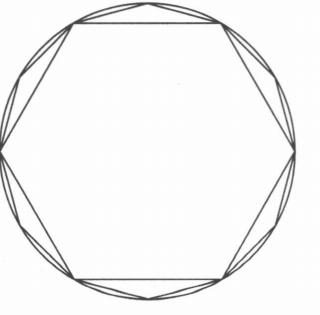
\includegraphics[width=.38\linewidth]{figures/lower/ch13/fig-13-2.png}

图 13.2
\end{center}

刘徽的方法就是将 $a_n$ 累加以得到级数和 $\pi$ 的近似值。在图 13.2 中的正六边形的面积为 $S_1=a_1$，而在其每条边上的 6 个小三角形面积之和就是 $a_2=S_2-S_1$。

现在分析级数通项的渐近性态。为方便起见，令 $x_n=3\cdot2^{n-1}$，则有
\begin{equation}
\begin{aligned}
a_n&=S_n-S_{n-1}=x_n\left(\sin\frac{\pi}{x_n}-\frac12\sin\frac{2\pi}{x_n}\right)\\
&=x_n\sin\frac{\pi}{x_n}\left(1-\cos\frac{\pi}{x_n}\right)\\
&\sim\frac{\pi^3}{2}\cdot\frac1{x_n^2}=\frac{2\pi^3}{9}\left(\frac14\right)^n.
\end{aligned}
\tag{13.6}
\end{equation}
因此刘徽的级数 $\sum_{n=1}^{\infty}a_n$ 在渐近性态上相当于公比为 $\frac14$ 的几何级数。

类似地可以分析每次计算后的误差，这就是级数的余项：
\begin{equation}
\varepsilon_n=S-S_n=\pi\left(1-\frac{\sin(\pi/x_n)}{\pi/x_n}\right)\sim\frac{\pi^3}{6}\cdot\frac1{x_n^2}.
\tag{13.7}
\end{equation}
由这些分析已可得到有用的结论。首先，从 (13.7) 知道 $\varepsilon_{n+1}\sim\frac14\varepsilon_n$，这与上册的例题 8.7.1 的分析可谓异曲同工。其次，比较 (13.6) 和 (13.7) 可以知道
\begin{equation}
\varepsilon_n\sim\frac13a_n.
\tag{13.8}
\end{equation}
从而就可以建立外推公式
\begin{equation}
\pi\approx S_n+\frac13(S_n-S_{n-1})=S_{n-1}+\frac43(S_n-S_{n-1}).
\tag{13.9}
\end{equation}
例如根据参考文献 [4] 中的第 48 页，仿照刘徽计算出 96 边形和 192 边形的面积：
\[
S_5\approx3.139350203,\qquad S_6\approx3.141031951,
\]
然后用 (13.9) 就可以得到有显著改进的结果：
\[
\pi\approx S_6+\frac13(S_6-S_5)\approx3.141592534.
\]
从 [4] 还知道，刘徽在这一步也用了某种外推法，但究竟是什么方法则仍是中国数学史上的一个悬案\footnote{根据 [4]（第 48 页），刘徽计算的是 $100\pi$ 的近似值。他得到的 $S_5=313\frac{581}{625}$，$S_6=314\frac{64}{625}$，$S_6-S_5=\frac{105}{625}$，因此按照 (13.8) 的修正量为 $\frac{35}{625}$，而刘徽实际所用的修正量为 $\frac{36}{625}$，从而得到 $100\pi\approx314\frac{100}{625}=314.16$。}（关于外推法可以参看 [12]）。
\end{xexample}

\subsection{思考题}

这一小节的思考题主要用于对级数定义进行复习，对于其中的是非题，若回答“是”，则要作出证明，若回答“不是”，则要举出反例。

\begin{xthought}[1]
（例题 13.1.2 之续）设比赛开始时，乌龟在 Achilles 之前 $1000\,\mathrm m$，Achilles 的速度为 $10\,\mathrm{m/s}$，乌龟的爬行速度为 $0.1\,\mathrm{m/s}$。试将 Zeno 悖论中的论点转化为无穷级数求和问题，并计算出 Achilles 赶上乌龟所需要的时间。（本题表明：有了无穷级数的工具之后，Zeno 的这个悖论就不再是悖论了。）
\end{xthought}
\begin{xsolution}
Achilles 先跑到乌龟的初始位置需要
\[
 t_1=\frac{1000}{10}=100\ \text{s}.
\]
在这 $100$ 秒内，乌龟又前进 $10$ 米，所以 Achilles 再跑到这个新位置需要
\[
 t_2=\frac{10}{10}=1\ \text{s}.
\]
此后每一次所需时间都是前一次的 $0.1/10=1/100$，故
\[
 t_n=100\left(\frac1{100}\right)^{n-1}.
\]
因此追上所需总时间为收敛几何级数
\[
 \sum_{n=1}^{\infty}t_n
 =100\sum_{n=0}^{\infty}\left(\frac1{100}\right)^n
 =\frac{100}{1-1/100}
 =\frac{10000}{99}\ \text{s}.
\]
这也等于用相对速度直接计算所得的 $1000/(10-0.1)=10000/99$ 秒。
\end{xsolution}


\begin{xthought}[2]
设级数 $\sum a_n$ 与 $\sum b_n$ 均收敛（或发散），讨论下列级数的敛散性：
\[
\sum(a_n\pm b_n),\qquad \sum a_nb_n,\qquad \sum\frac{a_n}{b_n}\quad(b_n\neq0),
\]
又对于 $\sum a_n$ 和 $\sum b_n$ 均为正项级数情况讨论同样的问题。
\end{xthought}
\begin{xsolution}
先讨论一般项级数。

若 $\sum a_n$ 与 $\sum b_n$ 都收敛，则线性性给出
\[
 \sum(a_n+b_n),\qquad \sum(a_n-b_n)
\]
都收敛；但 $\sum a_nb_n$ 与 $\sum a_n/b_n$ 都不能由此判定。例如
\[
 a_n=b_n=\frac{(-1)^n}{\sqrt n}
\]
时两级数都收敛，而 $\sum a_nb_n=\sum 1/n$ 发散；若改取
\[
 a_n=\frac{(-1)^n}{n},\qquad b_n=\frac{(-1)^n}{n^2},
\]
则乘积级数绝对收敛。对于商，取 $a_n=b_n=(-1)^n/n$ 时 $a_n/b_n=1$，商级数发散；取
\[
 a_n=\frac{(-1)^n}{n^2},\qquad b_n=\frac{(-1)^n}{n}
\]
时商级数为 $\sum1/n$，仍发散，而若取 $a_n=(-1)^n/n^3$、$b_n=(-1)^n/n$，商级数为 $\sum1/n^2$，收敛。

若 $\sum a_n$ 与 $\sum b_n$ 都发散，则上述四种运算均无统一结论。例如 $a_n=b_n=1/n$ 时差级数为零而和级数发散；取 $a_n=1/n$、$b_n=-1/n$ 时和级数为零而差级数发散。乘积方面，$a_n=b_n=1/n$ 时乘积级数收敛，而 $a_n=b_n=1/\sqrt n$ 时乘积级数发散。商方面，$a_n=1/n,b_n=n$ 时商级数 $\sum1/n^2$ 收敛，而 $a_n=b_n=1/n$ 时商级数发散。

若两级数都是正项级数，则结论更强。两者都收敛时，$\sum(a_n\pm b_n)$ 都收敛；又因 $b_n$ 有界，存在 $M>0$ 使 $a_nb_n\leq Ma_n$，故 $\sum a_nb_n$ 收敛；商级数仍无统一结论，例如 $a_n=b_n=1/n^2$ 时发散，而 $a_n=1/n^4,b_n=1/n^2$ 时收敛。

若两正项级数都发散，则 $\sum(a_n+b_n)$ 必发散；差级数、乘积级数和商级数均无统一结论。差级数可由 $a_n=b_n=1/n$ 得到收敛例，也可由 $a_n=2/n,b_n=1/n$ 得到发散例；乘积与商的正项反例同上即可构造。
\end{xsolution}


\begin{xthought}[3]
对于级数 $\sum\max\{a_n,b_n\}$，$\sum\min\{a_n,b_n\}$ 继续上题的讨论。
\end{xthought}
\begin{xsolution}
有恒等式
\[
 \max\{a_n,b_n\}+\min\{a_n,b_n\}=a_n+b_n.
\]
对于一般项级数，即使 $\sum a_n$、$\sum b_n$ 都收敛，也不能推出最大值级数或最小值级数收敛。例如令
\[
 a_n=\frac{(-1)^n}{\sqrt n},\qquad b_n=-a_n.
\]
则两级数都收敛，但
\[
 \max\{a_n,b_n\}=\frac1{\sqrt n},\qquad
 \min\{a_n,b_n\}=-\frac1{\sqrt n},
\]
故两个新级数都发散。若原两级数都发散，则更无统一结论。

对于正项级数，若 $\sum a_n$、$\sum b_n$ 都收敛，则
\[
 0\leq\min\{a_n,b_n\}\leq\max\{a_n,b_n\}\leq a_n+b_n,
\]
所以最大值级数和最小值级数都收敛。

若两正项级数都发散，则最大值级数一定发散，因为 $\max\{a_n,b_n\}\geq a_n$。最小值级数则不一定：令
\[
 a_n=\begin{cases}1/n,&n\text{ 奇},\\1/n^2,&n\text{ 偶},\end{cases}
 \qquad
 b_n=\begin{cases}1/n^2,&n\text{ 奇},\\1/n,&n\text{ 偶},\end{cases}
\]
则 $\sum a_n$、$\sum b_n$ 都发散，而
\[
 \min\{a_n,b_n\}=\frac1{n^2}
\]
所成级数收敛。
\end{xsolution}


\begin{xthought}[4]
如果级数 $\sum(a_n+a_{n+1})$ 收敛，是否必可推出 $\sum a_n$ 收敛？在 $\sum a_n$ 是正项级数时，答案又是什么？
\end{xthought}
\begin{xsolution}
一般不能推出。取 $a_n=(-1)^n$，则对每个 $n$ 有
\[
 a_n+a_{n+1}=0,
\]
所以 $\sum(a_n+a_{n+1})$ 收敛，而 $\sum a_n$ 发散。

若 $\sum a_n$ 为正项级数，则可以推出收敛。因为
\[
 0\leq a_n\leq a_n+a_{n+1},
\]
由比较判别法，$\sum(a_n+a_{n+1})$ 收敛必推出 $\sum a_n$ 收敛。
\end{xsolution}


\begin{xthought}[5]
记 $S=1-1+1-1+\cdots$，并作以下计算：
\[
S=1-(1-1+1-1+\cdots)=1-S\Rightarrow S=\frac12,
\]
问：其中有何错误？又可在阅读第二组参考题 18 后再做此题。
\end{xthought}
\begin{xsolution}
错误在于把一个并不收敛的级数当作普通实数来使用了结合律、移项和线性运算。级数
\[
 1-1+1-1+\cdots
\]
的部分和依次为 $1,0,1,0,\ldots$，没有极限，所以它在通常意义下没有和 $S$。因此
\[
 S=1-(1-1+1-1+\cdots)
\]
这个等式本身就没有通常级数理论中的依据。

若采用后面定义的 Cesàro 求和，则该级数确实可求和为 $1/2$；但这与通常意义下的收敛是不同概念。
\end{xsolution}


\begin{xthought}[6]
讨论级数 $a_1-a_1+a_2-a_2+\cdots+a_n-a_n+\cdots$ 的敛散性。
\end{xthought}
\begin{xsolution}
记部分和为 $S_N$。则
\[
 S_{2n}=0,
 \qquad
 S_{2n-1}=a_n.
\]
因此该级数收敛的充分必要条件是 $a_n\to0$。当 $a_n\to0$ 时，奇数项部分和与偶数项部分和都趋于 $0$，故级数之和为 $0$；若 $a_n\not\to0$，则奇数项部分和不趋于 $0$，级数发散。
\end{xsolution}


\begin{xthought}[7]
如果对每个正整数 $p$ 均成立
\[
\lim_{n\to\infty}(a_{n+1}+a_{n+2}+\cdots+a_{n+p})=0,
\]
问：是否能由此推出级数 $\sum a_n$ 一定收敛？
\end{xthought}
\begin{xsolution}
不能。取 $a_n=1/n$。对任意固定的正整数 $p$，有
\[
 0<a_{n+1}+\cdots+a_{n+p}
 \leq \frac{p}{n+1}\longrightarrow0.
\]
所以题设条件对每个固定 $p$ 都成立，但调和级数 $\sum1/n$ 发散。

这里与 Cauchy 收敛准则的差别在于：Cauchy 准则要求在 $n>N$ 后对\emph{所有}正整数 $p$ 同时成立统一的小量估计，而本题只对每个固定 $p$ 分别取极限。
\end{xsolution}


\begin{xthought}[8]
设 $a_n<c_n<b_n$，$n=1,2,\ldots$，若已知级数 $\sum a_n$ 和 $\sum b_n$ 同时收敛（或发散），问：能否推出级数 $\sum c_n$ 收敛（或发散）？并请将你的结论与数列的夹逼定理（见上册 20 页）作比较。
\end{xthought}
\begin{xsolution}
若 $\sum a_n$ 和 $\sum b_n$ 都收敛，则可以推出 $\sum c_n$ 收敛。因为
\[
 0<c_n-a_n<b_n-a_n.
\]
而
\[
 \sum(b_n-a_n)=\sum b_n-\sum a_n
\]
收敛，且其各项为正，所以由比较判别法 $\sum(c_n-a_n)$ 收敛，从而
\[
 \sum c_n=\sum a_n+\sum(c_n-a_n)
\]
收敛。

若 $\sum a_n$ 和 $\sum b_n$ 都发散，则一般不能推出 $\sum c_n$ 的敛散性。例如取
\[
 a_n=-\frac1n,\qquad b_n=\frac1n.
\]
若 $c_n=0$，则 $\sum c_n$ 收敛；若 $c_n=1/(2n)$，则 $\sum c_n$ 发散，而且都满足 $a_n<c_n<b_n$。

若三者都是正项，则当上下两个级数都收敛时，直接由 $0<c_n<b_n$ 得到 $\sum c_n$ 收敛；当上下两个级数都发散时，由 $c_n>a_n>0$ 得到 $\sum c_n$ 发散。

与数列夹逼定理相比，这里的“上下级数都收敛”已经足以推出中间级数收敛，并不要求两个级数的和相同；原因是逐项差 $b_n-a_n>0$ 本身组成收敛正项级数。
\end{xsolution}


\begin{xthought}[9]
设 $\sum a_n$ 收敛于和 $S$，若对于每个 $n$ 将 $a_{2n-1}$ 和 $a_{2n}$ 两项作交换，证明所得的新级数收敛，并求其和。
\end{xthought}
\begin{xsolution}
设原级数部分和为 $S_n$，交换每一对相邻项后所得级数部分和为 $T_n$。则
\[
 T_{2n}=S_{2n}.
\]
又有
\[
 T_{2n-1}=S_{2n-2}+a_{2n}
 =S_{2n}-a_{2n-1}.
\]
因为原级数收敛于 $S$，故 $S_n\to S$ 且 $a_n\to0$。于是
\[
 T_{2n}\to S,
 \qquad
 T_{2n-1}\to S.
\]
所以重排后的级数仍收敛，且和仍为 $S$。
\end{xsolution}


\begin{xthought}[10]
设有收敛正项级数 $\sum a_n$，且对于每个正整数 $n$ 成立 $a_n\leq a_nR_n$，其中 $R_n$ 为第 $n$ 个余项，证明：$\sum a_n$ 实际上是有限和。
\end{xthought}
\begin{xsolution}
若 $a_n>0$，题设不等式
\[
 a_n\leq a_nR_n
\]
可约去 $a_n$，得到 $R_n\geq1$。但收敛级数的余项必满足 $R_n\to0$，故当 $n$ 充分大时不可能再有 $a_n>0$。

因此从某一项起必有 $a_n=0$；也就是说，这个所谓“收敛正项级数”实际上只有有限个非零项，是有限和。
\end{xsolution}


\section{正项级数}

从本节开始我们将主要关注级数的敛散性判别法。如果能够判定一个级数收敛，则原则上至少可以用数值方法来计算级数和的近似值。关于级数求和的内容则在 §16.2 中讨论。

正项级数的敛散性一般只需要从其部分和数列是否有界就可以解决，在这方面已经得到了许多丰富的成果。以下的前两个小节分别介绍比较判别法的一般形式和特殊形式，然后在 13.2.3 小节介绍 Cauchy 积分判别法、Cauchy 凝聚判别法、Sapagof（萨巴高夫）判别法和 Kummer（库默尔）判别法。

\subsection{比较判别法的一般形式}

首先列出比较判别法的几种常用形式，它们的证明见教科书。

\textbf{比较判别法的基本形式。}设正项级数 $\sum a_n$ 和 $\sum b_n$ 的通项之间满足条件 $a_n\leq b_n$，$n=1,2,\ldots$，则就有以下结论：
\begin{align}
&\sum b_n\ \text{收敛}\Longrightarrow\sum a_n\ \text{收敛}; \tag{13.10}\\
&\sum a_n\ \text{发散}\Longrightarrow\sum b_n\ \text{发散}. \tag{13.11}
\end{align}
注意其中关于两个级数通项之间的不等式关系只需要对充分大的 $n$ 成立即可。

我们称 (13.10) 中的 $\sum b_n$ 与 (13.11) 中的 $\sum a_n$ 为比较级数。一般常用的比较级数如
\[
\sum_{n=1}^{\infty}aq^n,\qquad \sum_{n=1}^{\infty}\frac1{n^p},\qquad \sum_{n=2}^{\infty}\frac1{n\ln^p n}
\]
等等。在使用比较判别法时经常需要知道以下“级别”关系（参见 2.7.1 小节）：
\[
\ln n\ll n^\varepsilon\ll a^n\ll n!\ll n^n\qquad(a>1,\ \varepsilon>0).
\]

\textbf{比较判别法的极限形式。}若对于正项级数 $\sum a_n$ 和 $\sum b_n$ 存在（广义）极限
\begin{equation}
c=\lim_{n\to\infty}\frac{b_n}{a_n},
\tag{13.12}
\end{equation}
则当 $0<c<+\infty$ 时正项级数 $\sum a_n$ 与 $\sum b_n$ 同敛散，当 $c=0$ 时可以从 $\sum a_n$ 收敛推出 $\sum b_n$ 收敛，或从 $\sum b_n$ 发散推出 $\sum a_n$ 发散，当 $c=+\infty$ 时有相反的结论。

比较判别法的极限形式表明，研究级数 $\sum a_n$ 的通项所成的数列 $\{a_n\}$ 当 $n\to\infty$ 时的渐近性态往往是值得做的分析工作，其中包括通项 $\{a_n\}$ 是否是无穷小量的初步观察，如果不是，则已经可以断定该级数发散。对于上面 $0<c<+\infty$ 的情况，可以称为等价量判别法。

\textbf{比较判别法的比值形式。}设对于正项级数 $\sum a_n$，$\sum b_n$ 的通项当 $n$ 充分大时成立不等式
\begin{equation}
\frac{a_{n+1}}{a_n}\leq\frac{b_{n+1}}{b_n},
\tag{13.13}
\end{equation}
则结论 (13.10) 与 (13.11) 成立。

在下一小节会看到，从 d'Alembert（达朗贝尔）判别法开始的许多判别法都是在取定某个 $\sum b_n$ 之后从 (13.13) 导出的比较判别法的特殊形式。

\subsection{比较判别法的特殊形式}

上一小节中的比较判别法有一个共同点，就是都需要有比较级数。如何对于给定的级数去寻找合适的比较级数往往是一个难题。\footnote{这里的第一个困难在于，由于事先不知道一个级数究竟是收敛还是发散，因此事先不知道是按照 (13.10) 还是 (13.11) 去寻找比较级数。这在原则上只能通过尝试和摸索来解决。}

一种新的思维方法是“守株待兔”：取定比较级数以导出简单易用的判别法。例如，一般教科书中的 Cauchy 根值判别法和 d'Alembert 比值判别法就是如此。它们都是用几何级数作为比较级数。区别在于 Cauchy 根值判别法是从 (13.10) 和 (13.11) 出发两边开 $n$ 次根得到，而 d'Alembert 比值判别法则从比值形式 (13.13) 推出。由于教科书中都有它们的介绍和比较，此处从略。

不难看出，这样得到的每一种判别法的能力必定有限，其适用范围为所取的比较级数所限定。例如，$p$ 级数的敛散性就不可能用 Cauchy 根值判别法或 d'Alembert 比值判别法来进行判定。利用数列收敛和发散的快慢概念，就很容易理解这种现象。（参见 2.7.1 小节关于无穷大量的“级别”概念，§4.4 中关于无穷小量和无穷大量的比较，以及 8.7.1 小节中关于收敛速度的讨论。）

具体来说，采用 $p$ 级数作为比较级数就得到 Raabe（拉比）判别法，采用 $\sum_{n=2}^{\infty}\frac1{n\ln^p n}$ 作为比较级数就得到 Bertrand（贝特朗）判别法和 Gauss 判别法。它们的证明都可以从 [18] 等书中找到，此外还有许多更为细致的讨论和发展可以参考 [53] 和其中的文献。

现在我们将上述几种判别法的使用方法列表如下。以下设 $\sum_{n=1}^{\infty}a_n$ 为正项级数。
\[
\begin{aligned}
\text{Cauchy 根值判别法：}\quad
&\lim_{n\to\infty}\sqrt[n]{a_n}=c,\\[-2pt]
&c<1\text{ 时级数收敛，}\quad c>1\text{ 时级数发散};\\[4pt]
\text{d'Alembert 判别法：}\quad
&\lim_{n\to\infty}\frac{a_{n+1}}{a_n}=d,\\[-2pt]
&d<1\text{ 时级数收敛，}\quad d>1\text{ 时级数发散};\\[4pt]
\text{Raabe 判别法：}\quad
&\lim_{n\to\infty}n\left(\frac{a_n}{a_{n+1}}-1\right)=r,\\[-2pt]
&r>1\text{ 时级数收敛，}\quad r<1\text{ 时级数发散};\\[4pt]
\text{Bertrand 判别法：}\quad
&\lim_{n\to\infty}\ln n\left[n\left(\frac{a_n}{a_{n+1}}-1\right)-1\right]=b,\\[-2pt]
&b>1\text{ 时级数收敛，}\quad b<1\text{ 时级数发散};\\[4pt]
\text{Gauss 判别法：}\quad
&\frac{a_n}{a_{n+1}}=1+\frac{\mu}{n}+\bigO\left(\frac1{n^{1+\varepsilon}}\right),\quad \varepsilon>0,\\[-2pt]
&\mu>1\text{ 时级数收敛，}\quad \mu\leq1\text{ 时级数发散}.
\end{aligned}
\]

\begin{xremark}
表中除 Cauchy 根值判别法外，所列出的判别法都基于对比值 $a_{n+1}/a_n$（或 $a_n/a_{n+1}$）的分析，因此都可以称为比值判别法。在 Gauss 判别法中的 $\mu=1$ 时级数发散的结论可以从 Bertrand 判别法得到。此外，若再考虑
\begin{equation}
\sum_{n=9}^{\infty}\frac1{n\ln n(\ln\ln n)^p},\quad
\sum_{n=9}^{\infty}\frac1{n\ln n\ln\ln n(\ln\ln\ln n)^p},\quad\ldots
\tag{13.14}
\end{equation}
等比较级数，就可以得到更为精细的判别法，统称为 Bertrand 判别法（见 [65]）。
\end{xremark}

\begin{xremark}
容易发现本小节列举的所有判别法中，除了 Cauchy 根值判别法之外，都只能用于 $\{a_n\}$ 为单调的情况，至少当 $n$ 充分大时必须单调，否则就不可能成功。在这个意义上可以说，它们都是通项单调减少的正项级数判别法。正因为如此，虽然 Cauchy 根值判别法只是以几何级数为比较级数得到的判别法，能力有限，但是它的适用范围不能为表中任何其他判别法所完全覆盖。一个典型例子是以 $a_n=2^{-n-(-1)^n}$ 为通项的级数 $\sum_{n=1}^{\infty}a_n$，其中
\[
\frac{a_{n+1}}{a_n}=\begin{cases}\frac18,&n\text{ 为奇数},\\2,&n\text{ 为偶数}.
\end{cases}
\]
由 $\lim_{n\to\infty}\sqrt[n]{a_n}=\frac12$ 知可用 Cauchy 根值判别法，但比值判别法都不行。
\end{xremark}

\begin{xremark}
在这方面还应当提到各种形式的对数判别法。这里只举出两种对数判别法的极限形式（此外还有非极限形式和上、下极限形式）：
\begin{enumerate}[label=\arabic*.]
\item 若对正项级数 $\sum a_n$ 存在极限
\begin{equation}
\lim_{n\to\infty}\frac{\ln(1/a_n)}{\ln n}=r',
\tag{13.15}
\end{equation}
则当 $r'>1$ 时级数收敛，而当 $r'<1$ 时级数发散。
\item 若对正项级数 $\sum a_n$ 存在极限
\begin{equation}
\lim_{n\to\infty}\frac{\ln[1/(na_n)]}{\ln\ln n}=b',
\tag{13.16}
\end{equation}
则当 $b'>1$ 时级数收敛，而当 $b'<1$ 时级数发散。
\end{enumerate}
这两种判别法与 Raabe 判别法和 Bertrand 判别法的关系恰如 Cauchy 根值判别法与 d'Alembert 判别法那样，即当后者有效时前者一定有效（见 13.2.5 小节题 12），但反之不成立（参见 [53]）。与根值判别法相同的是，对数判别法不依赖于级数中的比值 $a_{n+1}/a_n$，因此对于通项不是单调的正项级数仍然可能有效。
\end{xremark}

\subsection{其他判别法}

对正项级数来说，除了上面介绍的几个判别法之外，其他判别法还有很多。本小节中只列举其中的几种判别法，它们都含有新的思想。此外，最后还讨论了比较级数中的一个理论问题。

首先应当指出，建立在广义积分基础上的 Cauchy 积分判别法是非常有用的。它不依赖于比较级数。例如在 (13.14) 中的级数的敛散性都可以用它得到解决，但是不能用前面的那些判别法来判定。

\begin{xproposition}[13.2.1（Cauchy 积分判别法）]
设 $f$ 在 $[1,+\infty)$ 上单调减少，则级数 $\sum_{n=1}^{\infty}f(n)$ 与无穷限广义积分 $\int_1^{+\infty}f(x)\,\dd x$ 同敛散。
\end{xproposition}

\begin{xremark}
积分判别法只是面积原理的一个应用（见上册 371 页的题 10），证明从略。希望初学者要学习这种面积比较方法，它可以解决不少问题。
\end{xremark}

\begin{xproposition}[13.2.2（Cauchy 凝聚判别法）]
设 $\{a_n\}$ 是单调减少的正数数列，则正项级数 $\sum_{n=1}^{\infty}a_n$ 收敛的充分必要条件是凝聚项级数
\[
\sum_{n=0}^{\infty}2^na_{2^n}=a_1+2a_2+4a_4+\cdots+2^na_{2^n}+\cdots
\]
收敛。
\end{xproposition}
\begin{xproof}
由于该正项级数的通项单调减少，因此不等式
\[
2^{k-1}a_{2^k}\leq a_{2^{k-1}+1}+a_{2^{k-1}+2}+\cdots+a_{2^k}\leq2^{k-1}a_{2^{k-1}}
\]
对 $k\geq1$ 成立。注意不等式中间部分恰有 $2^{k-1}$ 项。取 $k$ 从 1 到 $n$ 并相加，即可得到
\[
\frac12\sum_{k=1}^{n}2^ka_{2^k}\leq a_2+a_3+\cdots+a_{2^n}\leq\sum_{k=0}^{n-1}2^ka_{2^k},
\]
可见原来的级数的部分和与凝聚项级数的部分和同时有界或无界。
\end{xproof}

\begin{xremark}
这里也不需要比较级数，建议读者对 $\sum_{n=1}^{\infty}\frac1{n^p}$，$\sum_{n=2}^{\infty}\frac1{n\ln^p n}$ 和 (13.14) 中的级数用 Cauchy 凝聚判别法一试。
\end{xremark}

讨论一个数列 $\{a_n\}$ 是否收敛于 0 是数学分析中的基本问题之一，具有多方面的应用。无穷级数已经为此提供了一种方法，这就是研究级数 $\sum_{n=1}^{\infty}a_n$ 是否收敛。若级数收敛，则就得到 $\lim_{n\to\infty}a_n=0$。容易理解这个方法不会很有效，若级数发散就不能作出任何结论。但是对于单调数列，则有下面好得多的结果。

\begin{xproposition}[13.2.3（Sapagof 判别法）]
设正数数列 $\{a_n\}$ 单调减少，则 $\lim_{n\to\infty}a_n=0$ 的充分必要条件是正项级数
\[
\sum_{n=1}^{\infty}\left(1-\frac{a_{n+1}}{a_n}\right)
\]
发散。
\end{xproposition}
\begin{xproof}
将题中的级数记为 $\sum_{n=1}^{\infty}b_n$，其中 $b_n=1-\frac{a_{n+1}}{a_n}$，$n=1,2,\ldots$。

由于正数数列 $\{a_n\}$ 单调减少，因此有极限 $\lim_{n\to\infty}a_n=a$。若 $a>0$，则
\[
b_n\leq\frac{a_n-a_{n+1}}a.
\]
由于 $\sum_{n=1}^{\infty}(a_n-a_{n+1})=\lim_{n\to\infty}(a_1-a_n)=a_1-a$，可见 $\sum_{n=1}^{\infty}b_n$ 收敛。若 $a=0$，则有
\[
\sum_{k=n+1}^{n+p}b_k=\sum_{k=n+1}^{n+p}\frac{a_k-a_{k+1}}{a_k}\geq\sum_{k=n+1}^{n+p}\frac{a_k-a_{k+1}}{a_{n+1}}=1-\frac{a_{n+p+1}}{a_{n+1}}.
\]
对每个给定的 $n$，利用 $a_n\to0$ 的条件，总可以取到充分大的 $p$，使上式大于 $\frac12$。由级数的 Cauchy 收敛准则（见 (13.5)）可知级数 $\sum_{n=1}^{\infty}b_n$ 发散。
\end{xproof}

\begin{xremark}
本命题有几种等价形式（见 [18] 第二卷的 375 小节之 6）：
\begin{enumerate}[label=(\arabic*)]
\item 设 $\{a_n\}$ 为单调增加的正数数列，则该数列与级数 $\sum_{n=1}^{\infty}\left(1-\frac{a_n}{a_{n+1}}\right)$ 同敛散（这种形式在各种教科书中出现最多）；
\item 若正项级数 $\sum_{n=1}^{\infty}a_n$ 的部分和数列为 $\{S_n\}$，则 $\sum_{n=1}^{\infty}a_n$ 与 $\sum_{n=1}^{\infty}\frac{a_n}{S_n}$ 同敛散。
\end{enumerate}
\end{xremark}

\begin{xremark}
应当指出，在下一节的变号级数敛散性判别法中，往往需要证明某个单调数列收敛于 0。这时命题 13.2.3 就是一个有用的工具。这样就可能将变号级数的敛散性判别问题归结为某个正项级数的敛散性判别问题，而关于后者的方法要丰富得多。此外，还可以看出，如数列极限理论中的例题 2.3.3（上册 28 页）这类经典性结果都可以看成为命题 13.2.3 的特例。
\end{xremark}

\begin{xproposition}[13.2.4（Kummer 判别法）]
\begin{enumerate}[label=(\arabic*)]
\item 正项级数 $\sum_{n=1}^{\infty}a_n$ 收敛的充分必要条件是存在正数数列 $\{b_n\}$ 和正数 $\delta$，使得当 $n$ 充分大时有
\begin{equation}
b_n\frac{a_n}{a_{n+1}}-b_{n+1}\geq\delta>0;
\tag{13.17}
\end{equation}
\item 正项级数 $\sum_{n=1}^{\infty}a_n$ 发散的充分必要条件是存在发散的正项级数 $\sum_{n=1}^{\infty}\frac1{b_n}$，使得当 $n$ 充分大时有
\begin{equation}
b_n\frac{a_n}{a_{n+1}}-b_{n+1}\leq0.
\tag{13.18}
\end{equation}
\end{enumerate}
\end{xproposition}
\begin{xproof}
(1) 先证充分性。不妨设条件 (13.17) 已对于 $n\geq1$ 成立。将它改写为 $0<\delta a_{n+1}\leq b_na_n-b_{n+1}a_{n+1}$，可见正数数列 $\{b_na_n\}$ 单调减少，因此有估计：
\[
\sum_{k=1}^{n}a_k\leq a_1+\frac1\delta\sum_{k=1}^{n-1}(b_ka_k-b_{k+1}a_{k+1})\leq a_1+\frac1\delta b_1a_1,
\]
从而知级数 $\sum_{n=1}^{\infty}a_n$ 收敛。

再证必要性。在 $\sum_{n=1}^{\infty}a_n$ 收敛时记其余项为 $R_n$，$n\geq1$。令 $b_n=R_n/a_n$，则就有
\[
b_n\frac{a_n}{a_{n+1}}-b_{n+1}=\frac{R_n}{a_{n+1}}-\frac{R_{n+1}}{a_{n+1}}=\frac{R_n-R_{n+1}}{a_{n+1}}=1.
\]
因此取 $\delta=1$ 即可。

(2) 这时的充分性就是比较判别法的比值形式（见 (13.13)）。再证必要性。设 $\sum_{n=1}^{\infty}a_n$ 发散，取 $b_n=S_n/a_n$，其中 $S_n$ 为级数的第 $n$ 个部分和。这时 (13.18) 满足：
\[
b_n\frac{a_n}{a_{n+1}}-b_{n+1}=\frac{S_n-S_{n+1}}{a_{n+1}}=-1<0.
\]
从 $1/b_n=a_n/S_n$ 和命题 13.2.3（注 1 之 (2)）可知 $\sum_{n=1}^{\infty}1/b_n$ 发散。
\end{xproof}

\begin{xremark}
值得注意：Kummer 判别法中的 (1) 来自于正项级数收敛的充分必要条件是其部分和数列有上界，而与比较判别法没有直接联系。（参见《美国数学月刊》(1995) 第 102 卷 817--818 页中的历史观点。）
\end{xremark}

\begin{xremark}
采取不同的 $\{b_n\}$，就可以从 Kummer 判别法得到上一小节的各种比值判别法（见 [18] 第二卷的 371 小节）。关于 Kummer 判别法的必要性结果取自《美国数学月刊》(1994) 第 101 卷 450--452 页。
\end{xremark}

在上一小节中已经提到，由于存在收敛（发散）速度不同的正项级数，因此用特定的比较级数得到的比较判别法的能力总是有限的。现在我们证明，对于比较判别法而言，不论是为了判定级数收敛，还是发散，都不可能存在万能的比较级数。

\begin{xproposition}[13.2.5]
\begin{enumerate}[label=(\arabic*)]
\item （Du Bois-Reymond（杜布瓦-雷蒙）定理）对于一个给定的收敛正项级数 $\sum_{n=1}^{\infty}a_n$，一定存在一个收敛正项级数 $\sum_{n=1}^{\infty}b_n$，使得 $\lim_{n\to\infty}a_n/b_n=0$；
\item （Abel 定理）对于一个给定的发散正项级数 $\sum_{n=1}^{\infty}a_n$，一定存在一个发散正项级数 $\sum_{n=1}^{\infty}b_n$，使得 $\lim_{n\to\infty}b_n/a_n=0$。
\end{enumerate}
\end{xproposition}
\begin{xproof}
(1) 由正项级数 $\sum_{n=1}^{\infty}a_n$ 收敛知，余项 $R_n$ 单调减少收敛于 0。令
\[
b_n=\sqrt{R_{n-1}}-\sqrt{R_n},
\]
其中记 $R_0=\sum_{n=1}^{\infty}a_n$。从
\[
\frac{a_n}{b_n}=\frac{R_{n-1}-R_n}{\sqrt{R_{n-1}}-\sqrt{R_n}}=\sqrt{R_{n-1}}+\sqrt{R_n}\to0
\]
和 $\sum_{k=1}^{n}b_k=\sqrt{R_0}-\sqrt{R_n}\leq\sqrt{R_0}$ 可见 $\sum_{n=1}^{\infty}b_n$ 为满足要求的收敛级数。\footnote{若 $\{R_n\}$ 从某项起为 0，则正项级数 $\sum a_n$ 为有限和，任何收敛正项级数都可以作为 $\sum b_n$，只要每个 $b_n>0$。}

(2) 令 $b_n=a_n/S_n$，然后引用命题 13.2.3（注 1 之 (2)）即可。
\end{xproof}

\begin{xremark}
利用上册 §2.4 的 Stolz 定理，可以如下解释本题的结果。对于 (1)，分别记 $\sum a_n$ 和 $\sum b_n$ 的余项为 $R_n$ 和 $R'_n$，$n=1,2,\ldots$，则它们都是单调减少的无穷小量。由条件 $b_n>0$ 还知 $\{R'_n\}$ 严格单调减少。利用命题 2.4.2（$0/0$ 型的 Stolz 定理），可见有
\[
\lim_{n\to\infty}\frac{R_n}{R'_n}=\lim_{n\to\infty}\frac{R_n-R_{n+1}}{R'_n-R'_{n+1}}=\lim_{n\to\infty}\frac{a_n}{b_n}=0,
\]
从而 $R_n=\littleo(R'_n)$，这就是收敛级数 $\sum a_n$ 的收敛速度比 $\sum b_n$ 的收敛速度慢的严格表述。

对于 (2)，若分别记 $\sum a_n$ 和 $\sum b_n$ 的部分和为 $S_n$ 和 $S'_n$，$n=1,2,\ldots$，则它们都是单调增加的正无穷大量，而且 $\{S_n\}$ 还是严格单调增加的。用命题 2.4.3（$*/\infty$ 型的 Stolz 定理）就得到
\[
S'_n=\littleo(S_n),
\]
也就是 $S'_n\ll S_n$。这是作为正无穷大量的 $S'_n$ 的发散速度慢于 $S_n$ 的严格表述。
\end{xremark}

\subsection{例题}

先介绍对 $p$ 级数的敛散性证明，它们与上册已有的方法不同。其中第一个证明在方法论上很有价值。

\begin{xexample}[13.2.1]
讨论 $p$ 级数的敛散性。
\end{xexample}
\begin{xsolution}
\textbf{解 1}\quad 对于 $p\leq1$ 只需讨论 $p=1$，即调和级数。利用微分中值定理，有
\[
\ln\left(1+\frac1n\right)=\ln(n+1)-\ln n=\frac1{n+\theta}<\frac1n,
\]
其中 $0<\theta<1$，因此对调和级数的部分和有估计（参见上册 43 页）：
\[
\sum_{n=1}^{N}\frac1n>\ln2+(\ln3-\ln2)+\cdots+[\ln(N+1)-\ln N]=\ln(N+1),
\]
可见级数发散。对于 $p>1$ 同样有
\[
\frac1{n^{p-1}}-\frac1{(n+1)^{p-1}}=\frac{p-1}{(n+\theta)^p}>\frac{p-1}{(n+1)^p},
\]
其中 $0<\theta<1$，因此有估计
\[
\begin{aligned}
\sum_{n=1}^{N}\frac1{n^p}
&<1+\frac1{p-1}\left[\left(1-\frac1{2^{p-1}}\right)+\cdots+\left(\frac1{N^{p-1}}-\frac1{(N+1)^{p-1}}\right)\right]\\
&=1+\frac1{p-1}\left(1-\frac1{(N+1)^{p-1}}\right)<1+\frac1{p-1}=\frac p{p-1},
\end{aligned}
\]
可见级数收敛。

\textbf{解 2}\quad 对于 $p\leq1$ 只需证明 $p=1$ 时调和级数发散，用反证法：若调和级数收敛，其和为 $S$，则
\[
\begin{aligned}
S&=\left(1+\frac13+\cdots+\frac1{2n-1}+\cdots\right)+\left(\frac12+\frac14+\cdots+\frac1{2n}+\cdots\right)\\
&=\left(1+\frac13+\cdots+\frac1{2n-1}+\cdots\right)+\frac12\left(1+\frac12+\cdots+\frac1n+\cdots\right)\\
&=\left(1+\frac13+\cdots+\frac1{2n-1}+\cdots\right)+\frac S2,
\end{aligned}
\]
因此得到
\[
1+\frac13+\cdots+\frac1{2n-1}+\cdots=\frac S2=\frac12+\frac14+\cdots+\frac1{2n}+\cdots.
\]
但从 $1>\frac12$，$\frac13>\frac14$，$\ldots$，$\frac1{2n-1}>\frac1{2n}$，$\ldots$ 可见这不可能成立。

再讨论 $p>1$，这时级数的部分和数列 $\{S_n\}$ 满足条件 $S_{2N}<S_{2N+1}$ 以及
\[
\begin{aligned}
S_{2N+1}&=1+\left(\frac1{2^p}+\frac1{4^p}+\cdots+\frac1{(2N)^p}\right)+\left(\frac1{3^p}+\frac1{5^p}+\cdots+\frac1{(2N+1)^p}\right)\\
&<1+2\left(\frac1{2^p}+\frac1{4^p}+\cdots+\frac1{(2N)^p}\right)
=1+2^{1-p}\left(1+\frac1{2^p}+\cdots+\frac1{N^p}\right)\\
&<1+2^{1-p}S_{2N+1},
\end{aligned}
\]
因此部分和数列 $\{S_n\}$ 以 $1/(1-2^{1-p})$ 为上界，可见级数收敛。
\end{xsolution}

\begin{xremark}
证 2 见 \textit{Math. Magazine} (1979) 第 52 卷 178 页。
\end{xremark}

下面是利用 $p$ 级数为比较级数的几个例题。

\begin{xexample}[13.2.2]
讨论下列级数的敛散性：
\[
\text{(1) }\sum_{n=1}^{\infty}\frac1{3^{\ln n}};\qquad
\text{(2) }\sum_{n=2}^{\infty}\frac1{(\ln n)^{\ln n}};\qquad
\text{(3) }\sum_{n=3}^{\infty}\frac1{(\ln n)^{\ln\ln n}}.
\]
\end{xexample}
\begin{xsolution}
只要知道对于任何两个正数 $a,b>0$ 均成立
\[
a^{\ln b}=(\ee^{\ln a})^{\ln b}=\ee^{\ln a\ln b}=(\ee^{\ln b})^{\ln a}=b^{\ln a},
\]
就不难解决前两题。在题 (1) 中，利用 $3^{\ln n}=n^{\ln3}$ 和 $\ln3>1$，可见这个级数本身就是 $p>1$ 的 $p$ 级数，因此收敛。对于题 (2)，利用 $(\ln n)^{\ln n}=n^{\ln\ln n}$ 和当 $n$ 充分大时有 $n^{\ln\ln n}>n^2$，就可用 $\sum_{n=1}^{\infty}1/n^2$ 为比较级数而知其收敛。类似地在题 (3) 中有
\[
(\ln n)^{\ln\ln n}=\ee^{(\ln\ln n)^2}<\ee^{\ln n}=n,
\]
因此可从 $\sum_{n=1}^{\infty}1/n$ 的发散性知其发散。
\end{xsolution}

在下面的例子中用等价量判别法（当然也可用其他比较判别法）。

\begin{xexample}[13.2.3]
讨论下列级数的敛散性：
\[
\text{(1) }\sum_{n=1}^{\infty}\left[\frac{(2n-1)!!}{(2n)!!}\right]^k;\qquad
\text{(2) }\sum_{n=1}^{\infty}n!\left(\frac an\right)^n\ (a>0);\qquad
\text{(3) }\sum_{n=1}^{\infty}\left[\ee-\left(1+\frac1n\right)^n\right]^n.
\]
\end{xexample}
\begin{xsolution}
(1) 利用关于阶乘的 Wallis 公式知道有
\[
\frac{(2n)!!}{(2n-1)!!}\sim\sqrt{\pi n}
\]
（即公式 (11.29)），因此该级数的通项 $a_n$ 与级数 $\sum_{n=1}^{\infty}\frac1{(\pi n)^{k/2}}$ 的通项为等价无穷小量。从而知道级数当 $k\leq2$ 时发散，而当 $k>2$ 时收敛。

(2) 根据 Stirling 公式 (11.32)，可见成立
\[
a_n=n!\left(\frac an\right)^n\sim\left(\frac a\ee\right)^n\sqrt{2\pi n}=b_n.
\]
若 $a\geq\ee$，则可看出数列 $\{b_n\}$ 不是无穷小量，因此级数 $\sum b_n$ 以及 $\sum a_n$ 均发散。否则，可以取 $r\in(a/\ee,1)$，并看出
\[
\lim_{n\to\infty}\frac{a_n}{r^n}=0,
\]
因此从几何级数 $\sum_{n=1}^{\infty}r^n$（$0<r<1$）收敛知 $\sum_{n=1}^{\infty}a_n$ 收敛。

(3) 利用 Taylor 公式即可得到
\[
\ee-\left(1+\frac1n\right)^n=\frac{\ee}{2n}+\bigO\left(\frac1{n^2}\right)
\]
（见上册 230 页例题 8.1.4 之解 2），因此知级数收敛。
% SOURCE-ERR: 原书此处作“因此知级数发散”，由上式可确定应为“收敛”。
\end{xsolution}

下面是应用 Sapagof 判别法（命题 13.2.3）的一个典型例题。

\begin{xexample}[13.2.4]
问：在什么条件下数列 $\{a_n\}$ 为无穷小量，其中
\[
a_n=\binom{\alpha}{n}=\frac{\alpha(\alpha-1)\cdots(\alpha-n+1)}{n!},\qquad n=1,2,\ldots.
\]
\end{xexample}
\begin{xsolution}
从定义可见，若参数 $\alpha$ 为非负整数，则数列至多只有前有限项不等于 0，因此是无穷小量。否则，只需讨论 $\{|a_n|\}$。从
\[
\frac{|a_{n+1}|}{|a_n|}=\frac{n-\alpha}{n+1}=1-\frac{\alpha+1}{n+1}
\]
可见当 $\alpha\leq-1$ 时有 $|a_{n+1}|\geq|a_n|$，因此数列不可能趋于 0。

当 $\alpha>-1$ 时 $\{|a_n|\}$ 当 $n$ 充分大时单调减少。利用命题 13.2.3，从
\[
1-\frac{|a_{n+1}|}{|a_n|}=\frac{\alpha+1}{n+1}
\]
和级数 $\sum_{n=1}^{\infty}\frac{\alpha+1}{n+1}$ 发散可知 $\lim_{n\to\infty}a_n=0$。
\end{xsolution}

下面是在例题 13.2.1 中引进的微分中值定理方法的又一个应用。

\begin{xexample}[13.2.5]
设 $\sum_{n=1}^{\infty}a_n$ 为正项级数，$\{S_n\}$ 为其部分和数列，$p>1$，证明：无论 $\sum_{n=1}^{\infty}a_n$ 收敛与否，级数 $\sum_{n=1}^{\infty}\frac{a_n}{S_n^p}$ 总是收敛的。
\end{xexample}
\begin{xproof}
这里的出发点是 $a_n/S_n^p=(S_n-S_{n-1})/S_n^p$。设 $0<a<b$，对函数 $x^{1-p}$ 在区间 $[a,b]$ 上用 Lagrange 微分中值定理，可知存在 $\xi\in(a,b)$，使成立
\[
\frac1{a^{p-1}}-\frac1{b^{p-1}}=\frac{p-1}{\xi^p}(b-a)>(p-1)\frac{b-a}{b^p}.
\]
用 $a=S_{n-1}$，$b=S_n$ 代入，得到不等式
\[
\frac{a_n}{S_n^p}=\frac{S_n-S_{n-1}}{S_n^p}<\frac1{p-1}\left(\frac1{S_{n-1}^{p-1}}-\frac1{S_n^{p-1}}\right).
\]
由此可以作出级数 $\sum_{n=1}^{\infty}\frac{a_n}{S_n^p}$ 的部分和数列的上界估计：
\[
\begin{aligned}
\sum_{k=1}^{n}\frac{a_k}{S_k^p}
&=\frac1{a_1^{p-1}}+\sum_{k=2}^{n}\frac{a_k}{S_k^p}\\
&<\frac1{a_1^{p-1}}+\frac1{p-1}\sum_{k=2}^{n}\left(\frac1{S_{k-1}^{p-1}}-\frac1{S_k^{p-1}}\right)\\
&<\frac1{a_1^{p-1}}+\frac1{p-1}\frac1{a_1^{p-1}}
=\frac p{p-1}\frac1{a_1^{p-1}},
\end{aligned}
\]
因此级数 $\sum_{n=1}^{\infty}\frac{a_n}{S_n^p}$ 收敛。
\end{xproof}

\begin{xremark}
以上证明对于 $\sum a_n$ 收敛和发散情况都有效，但可以看出，若 $\sum a_n$ 收敛，记其和为 $S$，则 $a_n/S_n^p\sim a_n/S^p$，因此本题的结论是平凡的。
\end{xremark}

\begin{xexample}[13.2.6]
若正项级数 $\sum_{n=1}^{\infty}\frac1{a_n}$ 收敛，证明：级数 $\sum_{n=1}^{\infty}\frac{n}{a_1+a_2+\cdots+a_n}$ 也收敛。
\end{xexample}
\begin{xproof}
从条件可见正数数列 $\{a_n\}$ 为正无穷大量。以下分两步来做。

(1) 若数列 $\{a_n\}$ 单调增加，则有
\[
a_1+a_2+\cdots+a_{2n-1}\geq a_n+a_{n+1}+\cdots+a_{2n-1}\geq na_n,
\]
因此有不等式：
\[
\frac{2n-1}{a_1+\cdots+a_{2n-1}}+\frac{2n}{a_1+\cdots+a_{2n}}
\leq\frac{2n-1}{na_n}+\frac{2n}{na_n}<\frac4{a_n}.
\]
从而级数 $\sum_{n=1}^{\infty}\frac{n}{a_1+\cdots+a_n}$ 的部分和数列有上界，因此收敛。同时还得到
\begin{equation}
\sum_{n=1}^{\infty}\frac{n}{a_1+a_2+\cdots+a_n}\leq4\sum_{n=1}^{\infty}\frac1{a_n}.
\tag{13.19}
\end{equation}

(2) 对于一般情况，将数列 $\{a_n\}$ 按照从小到大重排\footnote{为实现这样的重排需反复用一个初等结论：若数列为正无穷大量，则数列中必有最小数。简证如下：设 $a_n\to+\infty$，则有 $N$，当 $n>N$ 时 $a_n>a_1$。于是 $\min\{a_1,a_2,\ldots,a_N\}$ 就是 $\{a_n\}$ 的最小数。}，并将重排后的数列记为 $\{b_n\}$。根据收敛的正项级数在重排后仍收敛，因此级数 $\sum_{n=1}^{\infty}1/b_n$ 收敛。利用 (1) 知道级数 $\sum_{n=1}^{\infty}\frac{n}{b_1+\cdots+b_n}$ 收敛。同时容易看出对于每个 $n$ 成立不等式\footnote{由于 $b_1,b_2,\ldots,b_n$ 是数列 $\{a_n\}$ 中按照从小到大的顺序重新排列的前 $n$ 项，因此它们的和不会大于任何其他 $n$ 项之和，其中包括 $a_1+a_2+\cdots+a_n$。}
\begin{equation}
b_1+b_2+\cdots+b_n\leq a_1+a_2+\cdots+a_n.
\tag{13.20}
\end{equation}
因此就有
\[
\frac{n}{a_1+a_2+\cdots+a_n}\leq\frac{n}{b_1+b_2+\cdots+b_n},
\]
于是从比较判别法就知道级数 $\sum_{n=1}^{\infty}\frac{n}{a_1+a_2+\cdots+a_n}$ 收敛。
\end{xproof}

\begin{xremark}
从 Knopp（克诺普）的论文（\textit{Math. Zeitschr.} (1929) 第 30 卷 387--413 页）知道 (13.19) 右边的常数 4 可以降低，其最优值为 2。
\end{xremark}

可以看出上题中第二个级数的第 $n$ 项是第一个级数的前 $n$ 项的调和平均值。根据几何平均值--调和平均值不等式（见上册第 8 页 1.3.2 小节题 3），可见该题是以下著名不等式的一个推论。

\begin{xexample}[13.2.7（Carleman 不等式）]
设 $\sum_{n=1}^{\infty}a_n$ 为收敛的正项级数，则成立
\[
\sum_{n=1}^{\infty}\sqrt[n]{a_1a_2\cdots a_n}<\ee\sum_{n=1}^{\infty}a_n,
\]
其中右边的系数 $\ee$ 不能再改进。
\end{xexample}
\begin{xproof}
对部分和估计如下（其中利用的不等式 $((n+1)/\ee)^n<n!$ 见上册 46 页题 7）：
\[
\begin{aligned}
\sum_{n=1}^{N}\sqrt[n]{a_1a_2\cdots a_n}
&=\sum_{n=1}^{N}\frac{\sqrt[n]{(a_1)(2a_2)\cdots(na_n)}}{\sqrt[n]{n!}}\\
&\leq\sum_{n=1}^{N}\frac{a_1+2a_2+\cdots+na_n}{n\sqrt[n]{n!}}\\
&\leq\ee\sum_{n=1}^{N}\frac{a_1+2a_2+\cdots+na_n}{n(n+1)}\\
&=\ee\sum_{n=1}^{N}\frac1{n(n+1)}\sum_{k=1}^{n}ka_k\\
&=\ee\sum_{k=1}^{N}ka_k\sum_{n=k}^{N}\frac1{n(n+1)}
=\ee\sum_{k=1}^{N}ka_k\left(\frac1k-\frac1{N+1}\right)\\
&\leq\ee\sum_{k=1}^{N}a_k.
\end{aligned}
\]
然后令 $N\to\infty$ 即可得到 Carleman 不等式。最后，对于每个 $N$ 构造一个数列：$a_n=1/n$，$n=1,2,\ldots,N$，而 $a_n=0$，$\forall n>N$，然后作出由 $\{a_n\}$ 得到的两个级数和之比，令 $N\to\infty$，且用 Stolz 定理和上册例题 2.5.3 的结果，就有
\[
\lim_{N\to\infty}\frac{\sum_{n=1}^{N}\sqrt[n]{a_1a_2\cdots a_n}}{\sum_{n=1}^{N}a_n}
=\lim_{N\to\infty}\frac{N}{\sqrt[N]{N!}}=\ee.
\]
这表明不等式右边的系数 $\ee$ 不能再改进。
\end{xproof}

\begin{xremark}
在《数学译林》(2004) 第 4 期中的一文给出了 Carleman 不等式的 5 个证明。在上述证明中的二重求和的顺序交换也可以利用裂项法改写为
\[
\frac1{n(n+1)}\sum_{k=1}^{n}ka_k=\frac1n\sum_{k=1}^{n}ka_k-\frac1{n+1}\sum_{k=1}^{n+1}ka_k+a_{n+1},
\]
并对于 $n=1,2,\ldots,N$ 相加，就得到同样的结果：
\[
\sum_{n=1}^{N}\frac1{n(n+1)}\sum_{k=1}^{n}ka_k\leq a_1+a_2+\cdots+a_N.
\]
\end{xremark}

\begin{xremark}
与此有关的还有 Hardy（哈代）不等式，其中当 $p>1$ 时为
\[
\sum_{n=1}^{\infty}\left(\frac1n\sum_{k=1}^{n}a_k^{1/p}\right)^p\leq\left(\frac p{p-1}\right)^p\sum_{n=1}^{\infty}a_n.
\]
令 $p\to+\infty$ 就导出 Carleman 不等式。
\end{xremark}

\subsection{练习题}

\begin{xexercise}[1]
设正项级数 $\sum_{n=1}^{\infty}a_n$ 和 $\sum_{n=1}^{\infty}b_n$ 的通项为等价量：$a_n\sim b_n$，又记两个级数的部分和为 $S_n$ 和 $S'_n$，余项为 $R_n$ 和 $R'_n$，$n=1,2,\ldots$，证明：
\begin{enumerate}[label=(\arabic*)]
\item 若两个级数均收敛，则 $R_n\sim R'_n$；
\item 若两个级数均发散，则 $S_n\sim S'_n$。
\end{enumerate}
\end{xexercise}
\begin{xsolution}
由 $a_n\sim b_n$，有 $a_n/b_n\to1$。

(1) 两级数都收敛时，$R_n\to0$，$R'_n\to0$，且
\[
 R_n-R_{n+1}=a_{n+1},\qquad R'_n-R'_{n+1}=b_{n+1}.
\]
因为 $R'_n$ 严格减少趋于 $0$，由 $0/0$ 型 Stolz 定理，
\[
 \lim_{n\to\infty}\frac{R_n}{R'_n}
 =\lim_{n\to\infty}\frac{R_n-R_{n+1}}{R'_n-R'_{n+1}}
 =\lim_{n\to\infty}\frac{a_{n+1}}{b_{n+1}}=1.
\]
故 $R_n\sim R'_n$。

(2) 两级数都发散时，正项级数的部分和满足 $S_n,S'_n\to+\infty$。由 $\infty/\infty$ 型 Stolz 定理，
\[
 \lim_{n\to\infty}\frac{S_n}{S'_n}
 =\lim_{n\to\infty}\frac{S_n-S_{n-1}}{S'_n-S'_{n-1}}
 =\lim_{n\to\infty}\frac{a_n}{b_n}=1.
\]
所以 $S_n\sim S'_n$。
\end{xsolution}


\begin{xexercise}[2]
设 $\sum a_n$ 为正项级数，证明：任意改变其中各项的顺序和加括号后得到的级数与原来的级数具有相同的敛散性，且在收敛时级数的和不变。（这表明，如果无限项求和时每项为非负数，或至多只有有限项为负数，则有限项求和时的结合律和交换律对于无限项求和都依然成立。）
\end{xexercise}
\begin{xsolution}
设原正项级数的部分和为 $S_n$。

若 $\sum a_n$ 收敛于 $S$，则任取 $\varepsilon>0$，可取 $N$ 使
\[
 \sum_{n>N}a_n<\varepsilon.
\]
任意重排后，只要新部分和已经包含原来的前 $N$ 项，它与 $S$ 的差就只由原级数第 $N$ 项以后的若干正项组成，故小于 $\varepsilon$。因此任意重排仍收敛于 $S$。加括号只是取重排后部分和数列的一个子列，也仍趋于 $S$。

若原级数发散，则 $S_n\to+\infty$。任意重排后的部分和仍是若干原级数正项之和。给定 $M>0$，先取原级数有限个项使其和大于 $M$；重排后这些有限项终会全部出现，于是从某个部分和起，新部分和大于 $M$。故重排后仍发散于 $+\infty$。加括号后的部分和是原部分和中的递增子列，也发散于 $+\infty$。

所以任意重排、任意加括号都保持敛散性；在收敛情形和不变。
\end{xsolution}


\begin{xexercise}[3]
讨论下列各级数的敛散性：
\[
\begin{array}{ll}
(1)\ \displaystyle\sum_{n=1}^{\infty}\frac1{3^{\sqrt n}};&
(2)\ \displaystyle\sum_{n=1}^{\infty}\frac1{n^{1+1/n}};\\[6pt]
(3)\ \displaystyle\sum_{n=1}^{\infty}\left[\frac1n-\ln\left(1+\frac1n\right)\right];&
(4)\ \displaystyle\sum_{n=1}^{\infty}\frac{n^{n-1}}{(2n^2+n+1)^{(n-1)/2}};\\[6pt]
(5)\ \displaystyle\sum_{n=2}^{\infty}\frac{n^{\ln n}}{(\ln n)^n};&
(6)\ \displaystyle\sum_{n=1}^{\infty}\frac{\ee^{-(1+1/2+\cdots+1/n)}}{n^p};\\[6pt]
(7)\ \displaystyle\sum_{n=1}^{\infty}\left(a^{1/n}-\frac{b^{1/n}+c^{1/n}}2\right)\quad(a,b,c>0);&
(8)\ \displaystyle\sum_{n=1}^{\infty}\left(1-\frac{\ln n}{n}\right)^n.
\end{array}
\]
\end{xexercise}
\begin{xsolution}
逐项讨论。

(1) 令 $k^2\leq n<(k+1)^2$。这一组至多有 $2k+1$ 项，且
\[
 \frac1{3^{\sqrt n}}\leq\frac1{3^k}.
\]
故该组之和不超过 $(2k+1)3^{-k}$，而 $\sum(2k+1)3^{-k}$ 收敛，所以原级数收敛。

(2)
\[
 \frac1{n^{1+1/n}}=\frac1n\,n^{-1/n}\sim\frac1n,
\]
因为 $n^{-1/n}\to1$。故级数发散。

(3) 利用
\[
 \ln(1+x)=x-\frac{x^2}{2}+\bigO(x^3),\qquad x\to0,
\]
得到
\[
 \frac1n-\ln\left(1+\frac1n\right)
 =\frac1{2n^2}+\bigO\left(\frac1{n^3}\right).
\]
故级数收敛。

(4) 记通项为 $u_n$。则
\[
 \sqrt[n]{u_n}
 =\left(\frac{n^2}{2n^2+n+1}\right)^{\frac{n-1}{2n}}
 \longrightarrow\frac1{\sqrt2}<1.
\]
由 Cauchy 根值判别法，级数收敛。

(5) 记通项为 $u_n$，则
\[
 \sqrt[n]{u_n}
 =\frac{n^{(\ln n)/n}}{\ln n}
 =\frac{\exp((\ln n)^2/n)}{\ln n}\longrightarrow0.
\]
故级数收敛。

(6) 记 $H_n=1+1/2+\cdots+1/n$。由
\[
 H_n=\ln n+\gamma+\littleo(1)
\]
可得
\[
 \frac{\ee^{-H_n}}{n^p}
 \sim \ee^{-\gamma}n^{-(p+1)}.
\]
因此级数当且仅当 $p>0$ 时收敛；当 $p\leq0$ 时发散。

(7) 令 $A=\ln a,B=\ln b,C=\ln c$。展开
\[
 a^{1/n}=1+\frac A n+\frac{A^2}{2n^2}+\bigO(n^{-3}),
\]
对 $b,c$ 同理，于是通项
\[
 u_n=\frac{A-(B+C)/2}{n}
 +\frac{A^2/2-(B^2+C^2)/4}{n^2}
 +\bigO(n^{-3}).
\]
若 $2A\neq B+C$，则 $u_n\sim[A-(B+C)/2]/n$，级数发散。若 $2A=B+C$，即 $a^2=bc$，则一阶项消失，$u_n=\bigO(n^{-2})$，级数绝对收敛。因此收敛的充分必要条件是
\[
 a^2=bc.
\]

(8) 对充分大的 $n$ 有 $0<\ln n/n<1$，且
\[
 n\ln\left(1-\frac{\ln n}{n}\right)
 =-\ln n+\littleo(1).
\]
所以
\[
 \left(1-\frac{\ln n}{n}\right)^n\sim\frac1n,
\]
故级数发散。
\end{xsolution}


\begin{xexercise}[4]
从例题 13.2.6 和 13.2.7 知道，若从收敛正项级数 $\sum_{n=1}^{\infty}a_n$ 作出 $\{u_n\}$，其中 $u_n$ 为 $a_1,a_2,\ldots,a_n$ 的调和平均值或几何平均值，则 $\sum_{n=1}^{\infty}u_n$ 收敛。但是若 $u_n$ 为算术平均值，则情况大不一样。证明：若正项级数 $\sum_{n=1}^{\infty}a_n$ 收敛，则除了一种特殊情况之外，级数 $\sum_{n=1}^{\infty}\frac{a_1+a_2+\cdots+a_n}{n}$ 必定发散。
\end{xexercise}
\begin{xsolution}
记 $S_n=a_1+\cdots+a_n$，并设 $\sum a_n=S$。正项且非零时 $S>0$，于是
\[
 \frac{S_n}{n}\sim\frac S n.
\]
故
\[
 \sum_{n=1}^{\infty}\frac{a_1+\cdots+a_n}{n}
\]
与调和级数同敛散，因而发散。

唯一的特殊情形是 $S=0$。对非负项级数这只可能发生在 $a_n=0$ 对所有 $n$ 成立，此时所给级数当然收敛（且各项全为零）。
\end{xsolution}


\begin{xexercise}[5]
试用 Sapagof 判别法（即命题 13.2.3）或其他方法证明下列数列收敛于 0：
\[
(1)\ \left\{\frac{(2n)!}{4^n(n!)^2}\right\};\qquad
(2)\ \left\{\frac{n^n}{\ee^n n!}\right\};\qquad
(3)\ \left\{\frac{n!}{(x+1)(x+2)\cdots(x+n)}\right\}\ (x>0).
\]
\end{xexercise}
\begin{xsolution}
(1) 令
\[
 u_n=\frac{(2n)!}{4^n(n!)^2}.
\]
则
\[
 \frac{u_{n+1}}{u_n}=\frac{2n+1}{2n+2}
 =1-\frac1{2n+2}.
\]
数列 $\{u_n\}$ 正且单调减少，而
\[
 \sum_{n=1}^{\infty}\left(1-\frac{u_{n+1}}{u_n}\right)
 =\sum_{n=1}^{\infty}\frac1{2n+2}
\]
发散。由 Sapagof 判别法，$u_n\to0$。

(2) 令
\[
 u_n=\frac{n^n}{\ee^n n!}.
\]
则
\[
 \frac{u_{n+1}}{u_n}
 =\frac1\ee\left(1+\frac1n\right)^n
 =1-\frac1{2n}+\bigO\left(\frac1{n^2}\right).
\]
故 $u_n$ 最终单调减少，且
\[
 1-\frac{u_{n+1}}{u_n}
 =\frac1{2n}+\bigO(n^{-2}).
\]
右端所成正项级数发散，由 Sapagof 判别法 $u_n\to0$。

(3) 令
\[
 u_n=\frac{n!}{(x+1)(x+2)\cdots(x+n)},\qquad x>0.
\]
则
\[
 \frac{u_{n+1}}{u_n}=\frac{n+1}{n+1+x}
 =1-\frac{x}{n+1+x}.
\]
故 $u_n$ 正且单调减少，而
\[
 \sum_{n=1}^{\infty}\frac{x}{n+1+x}
\]
发散。再由 Sapagof 判别法得到 $u_n\to0$。
\end{xsolution}


\begin{xexercise}[6]
举出一个收敛的正项级数 $\sum a_n$ 的例子，使它满足条件 $\limsup_{n\to\infty}na_n=1$。
\end{xexercise}
\begin{xsolution}
例如定义
\[
 a_n=\begin{cases}
 2^{-k},&n=2^k,\quad k=1,2,\ldots,\\
 n^{-2},&n\neq2^k.
 \end{cases}
\]
则
\[
 \sum_{n=1}^{\infty}a_n
 \leq\sum_{k=1}^{\infty}2^{-k}+\sum_{n=1}^{\infty}\frac1{n^2}<\infty.
\]
另一方面，在 $n=2^k$ 时有 $na_n=1$，而在非 $2$ 的幂处 $na_n=1/n\to0$，所以
\[
 \limsup_{n\to\infty}na_n=1.
\]
\end{xsolution}


\begin{xexercise}[7]
已知正项级数 $\sum a_n$ 收敛，$p>1$，证明：级数 $\sum a_n^p$ 一定收敛。又若去掉 $\sum a_n$ 为正项级数的条件，结论是否还成立？
\end{xexercise}
\begin{xsolution}
因为 $\sum a_n$ 是收敛正项级数，所以 $a_n\to0$。对充分大的 $n$ 有 $0<a_n\leq1$，于是当 $p>1$ 时
\[
 0<a_n^p\leq a_n.
\]
由比较判别法，$\sum a_n^p$ 收敛。

若去掉正项条件，结论不成立。例如
\[
 a_n=\frac{(-1)^n}{\sqrt n}
\]
所成级数收敛，但取 $p=2$ 时
\[
 \sum a_n^2=\sum\frac1n
\]
发散。
\end{xsolution}


\begin{xexercise}[8]
设数列 $\{a_n\}$ 单调减少收敛于 0，且 $b_n=a_n-2a_{n+1}+a_{n+2}>0$，$n=1,2,\ldots$；证明：级数 $\sum_{n=1}^{\infty}nb_n$ 收敛，且其和为 $a_1$。
\end{xexercise}
\begin{xsolution}
令
\[
 d_n=a_n-a_{n+1}\geq0.
\]
则 $b_n=d_n-d_{n+1}>0$，所以 $\{d_n\}$ 单调减少。又
\[
 \sum_{n=1}^{\infty}d_n=a_1<\infty,
\]
故由单调正项收敛级数的 Abel--Pringsheim 结论，$nd_n\to0$。

对部分和作求和分部：
\[
 \begin{aligned}
 \sum_{n=1}^{N}nb_n
 &=\sum_{n=1}^{N}n(d_n-d_{n+1})\\
 &=\sum_{n=1}^{N}d_n-Nd_{N+1}\\
 &=a_1-a_{N+1}-N(a_{N+1}-a_{N+2}).
 \end{aligned}
\]
令 $N\to\infty$，由 $a_{N+1}\to0$ 和 $Nd_{N+1}\to0$ 得
\[
 \sum_{n=1}^{\infty}nb_n=a_1.
\]
因此该级数收敛，且和为 $a_1$。
\end{xsolution}


\begin{xexercise}[9]
设对于每个正整数 $n$ 都有 $0<a_n<a_{2n}+a_{2n+1}$，证明：级数 $\sum_{n=1}^{\infty}a_n$ 发散。
\end{xexercise}
\begin{xsolution}
反设 $\sum a_n$ 收敛，记其和为 $S$。将题设不等式对 $n=1,\ldots,N$ 相加，得
\[
 \sum_{n=1}^{N}a_n
 <\sum_{n=1}^{N}(a_{2n}+a_{2n+1})
 \leq\sum_{k=2}^{2N+1}a_k.
\]
令 $N\to\infty$，左边趋于 $S$，右边趋于 $S-a_1$，于是得到
\[
 S\leq S-a_1,
\]
与 $a_1>0$ 矛盾。故 $\sum a_n$ 必发散。
\end{xsolution}


\begin{xexercise}[10]
设 $x>0$，证明：级数
\[
\sum_{n=1}^{\infty}\frac{x^n}{(1+x)(1+x^2)\cdots(1+x^n)}
\]
收敛。
\end{xexercise}
\begin{xsolution}
令
\[
 b_n=\frac1{(1+x)(1+x^2)\cdots(1+x^n)},
 \qquad b_0=1.
\]
则有精确的裂项关系
\[
 b_{n-1}-b_n
 =\frac{x^n}{(1+x)(1+x^2)\cdots(1+x^n)}.
\]
因此
\[
 \sum_{n=1}^{N}\frac{x^n}{(1+x)(1+x^2)\cdots(1+x^n)}
 =b_0-b_N<1.
\]
题中各项均为正数，故其部分和单调且有上界，所以对每个 $x>0$，级数均收敛。
\end{xsolution}


\begin{xexercise}[11]
设 $x>0$，讨论级数
\[
\sum_{n=1}^{\infty}(2-x)(2-x^{1/2})(2-x^{1/3})\cdots(2-x^{1/n})
\]
的敛散性。
\end{xexercise}
\begin{xsolution}
记
\[
 u_n=\prod_{k=1}^{n}(2-x^{1/k}).
\]
若 $x=2^m$（$m$ 为正整数），则当 $n\geq m$ 时乘积中出现因子 $2-x^{1/m}=0$，故级数实际上只有有限个非零项，必收敛。下面设 $x$ 不是 $2$ 的正整数次幂。

当 $k\to\infty$ 时
\[
 x^{1/k}=\exp\left(\frac{\ln x}{k}\right)
 =1+\frac{\ln x}{k}+\bigO\left(\frac1{k^2}\right),
\]
所以
\[
 2-x^{1/k}
 =1-\frac{\ln x}{k}+\bigO\left(\frac1{k^2}\right).
\]
从某项起这些因子为正，取对数得
\[
 \ln|u_n|
 =-\ln x\sum_{k=1}^{n}\frac1k+\bigO(1)
 =-(\ln x)\ln n+\bigO(1).
\]
因而存在常数 $C>0$ 使
\[
 |u_n|\sim Cn^{-\ln x}.
\]
而 $u_n$ 的符号从某项起固定，所以题中级数与正项 $p$ 级数具有相同敛散性。故在非零因子情形，它当且仅当
\[
 \ln x>1,
\]
即 $x>\ee$ 时收敛。

综合零因子情形，原级数的收敛范围为
\[
 \boxed{x=2\quad\text{或}\quad x>\ee}.
\]
（其余 $2^m$ 中 $m\geq2$ 已包含在 $x>\ee$ 内。）
\end{xsolution}


\begin{xexercise}[12]
设 $\sum_{n=1}^{\infty}a_n$ 为正项级数，证明：
\begin{enumerate}[label=(\arabic*)]
\item 若在 Raabe 判别法中的极限 $\lim_{n\to\infty}n\left(\frac{a_n}{a_{n+1}}-1\right)$ 存在，则在对数判别法 (13.15) 中的极限 $\lim_{n\to\infty}\frac{\ln(1/a_n)}{\ln n}$ 也存在，且极限值相同；
\item 若在 Bertrand 判别法中的极限 $\lim_{n\to\infty}\ln n\left[n\left(\frac{a_n}{a_{n+1}}-1\right)-1\right]$ 存在，则在对数判别法 (13.16) 中的极限 $\lim_{n\to\infty}\frac{\ln[1/(na_n)]}{\ln\ln n}$ 也存在，且极限值相同。
\end{enumerate}
\end{xexercise}
\begin{xsolution}
(1) 设
\[
 r=\lim_{n\to\infty}n\left(\frac{a_n}{a_{n+1}}-1\right).
\]
令
\[
 A_n=\ln\frac1{a_n},\qquad B_n=\ln n.
\]
由题设 $a_n/a_{n+1}\to1$，并且
\[
 n\ln\frac{a_n}{a_{n+1}}
 \sim n\left(\frac{a_n}{a_{n+1}}-1\right)\to r.
\]
另一方面
\[
 B_{n+1}-B_n=\ln\left(1+\frac1n\right)\sim\frac1n.
\]
故由 Stolz 定理
\[
 \lim_{n\to\infty}\frac{A_n}{B_n}
 =\lim_{n\to\infty}
 \frac{\ln(a_n/a_{n+1})}{\ln((n+1)/n)}=r.
\]
这正是 (13.15) 中的极限。

(2) 设 Bertrand 极限为 $b$，即
\[
 \ln n\left[n\left(\frac{a_n}{a_{n+1}}-1\right)-1\right]\to b.
\]
于是
\[
 \frac{a_n}{a_{n+1}}
 =1+\frac1n+\frac{b+\littleo(1)}{n\ln n}.
\]
令
\[
 A_n=\ln\frac1{na_n},\qquad B_n=\ln\ln n.
\]
则
\[
 \begin{aligned}
 A_{n+1}-A_n
 &=\ln\frac{na_n}{(n+1)a_{n+1}}\\
 &=\ln\left(\frac{a_n/a_{n+1}}{1+1/n}\right)
 =\frac{b+\littleo(1)}{n\ln n},
 \end{aligned}
\]
而
\[
 B_{n+1}-B_n
 =\ln\frac{\ln(n+1)}{\ln n}
 \sim\frac1{n\ln n}.
\]
再用 Stolz 定理得到
\[
 \lim_{n\to\infty}\frac{\ln[1/(na_n)]}{\ln\ln n}=b,
\]
即 (13.16) 的极限存在且与 Bertrand 极限相同。
\end{xsolution}


\begin{xexercise}[13]
设 $\sum_{n=1}^{\infty}a_n$ 为正项级数，$k$ 为一正整数，如果 $\lim_{n\to\infty}\frac{a_{n+k}}{a_n}=l$，证明：$l<1$ 时，$\sum a_n$ 收敛；$l>1$ 时，$\sum a_n$ 发散。（本题如取 $k=1$，就是 d'Alembert 判别法。因此本题可看作为 d'Alembert 判别法的一个推广。）
\end{xexercise}
\begin{xsolution}
若 $l<1$，取 $q$ 满足 $l<q<1$。当 $n$ 充分大时
\[
 a_{n+k}\leq q a_n.
\]
把级数按模 $k$ 的余数分成 $k$ 个子列。对每个 $r=1,\ldots,k$，从充分大的指标起有
\[
 a_{r+(j+1)k}\leq q a_{r+jk},
\]
故每个子列都被收敛几何级数控制。因此 $k$ 个子列之和均收敛，原级数收敛。

若 $l>1$，取 $q$ 满足 $1<q<l$。当 $n$ 充分大时
\[
 a_{n+k}\geq q a_n.
\]
于是沿任一固定模 $k$ 的子列，通项最终按至少公比 $q>1$ 增长，特别不可能趋于 $0$。故原级数发散。
\end{xsolution}


\begin{xexercise}[14]
（Dini（迪尼））设正项级数 $\sum_{n=1}^{\infty}a_n$ 收敛，其余项为 $R_n=\sum_{k=n+1}^{\infty}a_k$，$n=0,1,\ldots$。证明：$\sum_{n=1}^{\infty}\frac{a_n}{R_{n-1}}$ 发散，但对任意 $p>0$，$\sum_{n=1}^{\infty}\frac{a_n}{R_{n-1}^{1-p}}$ 收敛。
\end{xexercise}
\begin{xsolution}
记
\[
 x_n=\frac{a_n}{R_{n-1}}=1-\frac{R_n}{R_{n-1}},
 \qquad 0<x_n<1.
\]
因为 $R_n\downarrow0$，有
\[
 \prod_{k=1}^{n}(1-x_k)=\frac{R_n}{R_0}\longrightarrow0.
\]
若 $\sum x_n$ 收敛，则 $x_n\to0$，且 $-\ln(1-x_n)\sim x_n$，从而 $\sum[-\ln(1-x_n)]$ 收敛，乘积应收敛于非零值，矛盾。因此
\[
 \sum_{n=1}^{\infty}\frac{a_n}{R_{n-1}}
\]
发散。

再证第二个结论。题中通项为
\[
 \frac{a_n}{R_{n-1}^{1-p}}=a_nR_{n-1}^{p-1}.
\]
若 $p\geq1$，因 $R_{n-1}$ 有界，存在常数 $C$ 使
\[
 a_nR_{n-1}^{p-1}\leq Ca_n,
\]
故级数收敛。

若 $0<p<1$，对函数 $t^p$ 在 $[R_n,R_{n-1}]$ 上用中值定理，存在 $\xi_n\in(R_n,R_{n-1})$ 使
\[
 R_{n-1}^p-R_n^p=p\xi_n^{p-1}a_n.
\]
由于 $p-1<0$ 且 $\xi_n<R_{n-1}$，
\[
 \xi_n^{p-1}\geq R_{n-1}^{p-1},
\]
故
\[
 a_nR_{n-1}^{p-1}
 \leq\frac1p(R_{n-1}^p-R_n^p).
\]
右端可望远镜求和，所以对一切 $p>0$，
\[
 \sum_{n=1}^{\infty}\frac{a_n}{R_{n-1}^{1-p}}
\]
都收敛。
\end{xsolution}


\begin{xexercise}[15]
设 $0<a_1<\frac\pi2$，然后用迭代公式 $a_n=\sin a_{n-1}$ 生成数列 $\{a_n\}$，讨论级数 $\sum_{n=1}^{\infty}a_n^p$ 的敛散性（参考上册 233 页的例题 8.1.10）。
\end{xexercise}
\begin{xsolution}
由 $0<a_1<\pi/2$ 及 $\sin x<x$（$x>0$），数列 $a_n$ 正且严格减少，因此有极限 $L\geq0$。极限满足 $L=\sin L$，故 $L=0$。

当 $x\to0$ 时
\[
 \sin x=x-\frac{x^3}{6}+\bigO(x^5),
\]
从而
\[
 \frac1{\sin^2x}-\frac1{x^2}=\frac13+\bigO(x^2).
\]
代入 $x=a_n$ 得
\[
 \frac1{a_{n+1}^2}-\frac1{a_n^2}\longrightarrow\frac13.
\]
由 Stolz 定理
\[
 \lim_{n\to\infty}\frac{1/a_n^2}{n}=\frac13,
\]
即
\[
 a_n\sim\sqrt{\frac3n}.
\]
因此
\[
 a_n^p\sim3^{p/2}n^{-p/2}.
\]
与 $p$ 级数比较可知
\[
 \boxed{\sum_{n=1}^{\infty}a_n^p\text{ 当且仅当 }p>2\text{ 时收敛}.}
\]
当 $p\leq2$ 时发散（其中 $p\leq0$ 时通项甚至不趋于 $0$）。
\end{xsolution}


\section{一般项级数}

本节研究一般项级数，即在 $\sum_{n=1}^{\infty}a_n$ 中既有无限多个正项，又有无限多个负项的情况，称这样的级数为变号级数。对于其他情况则可归到正项级数的范畴去解决。

这里需要强调指出绝对收敛级数与条件收敛级数的区别。从敛散性来看，前者的收敛性可以用正项级数的各种判别法来判定，而后者则需要全新的判别法。从级数的一系列性质来看，两者均有极大的不同。粗略地说，前者与有限和相似，而后者则完全不同。

\subsection{一般项级数的敛散性判别法}

称收敛级数 $\sum a_n$ 为绝对收敛级数，若 $\sum|a_n|$ 也收敛；否则就称为条件收敛级数。用 Cauchy 收敛准则就可以得到这里的基本结论：

\begin{xproposition}[13.3.1]
若级数 $\sum_{n=1}^{\infty}|a_n|$ 收敛，则 $\sum_{n=1}^{\infty}a_n$ 必定收敛。
\end{xproposition}

由此可知，在研究变号级数 $\sum a_n$ 的敛散性时，可以先分析对应的正项级数 $\sum|a_n|$ 的敛散性。对后者来说可以用正项级数的各种判别法。若 $\sum|a_n|$ 收敛，则原来的级数 $\sum a_n$ 的收敛性就已经解决。若 $\sum|a_n|$ 发散，则 $\sum a_n$ 的敛散性有两种可能：条件收敛或发散。这时上一节中以比较判别法为基础的各种判别法都不能奏效。其中的例外是导出发散结论的 Cauchy 根值判别法和 d'Alembert 判别法。这就是说，在对 $\sum|a_n|$ 用这两种判别法时，若有
\[
\lim_{n\to\infty}\sqrt[n]{|a_n|}>1\quad\text{或}\quad
\lim_{n\to\infty}\frac{|a_{n+1}|}{|a_n|}>1,
\]
则可以肯定原来的级数 $\sum_{n=1}^{\infty}a_n$ 发散，其原因在于这两种判别法背后的比较级数是（正项）几何级数，它在公比大于 1 时的级数通项不收敛于 0，而 $\lim_{n\to\infty}|a_n|=0$ 与 $\lim_{n\to\infty}a_n=0$ 是等价的，因此它们的反面也等价。

变号级数中最基本的例子就是在上册 54 页例题 2.7.3 中的无穷级数：
\[
\sum_{n=1}^{\infty}\frac{(-1)^{n-1}}n=1-\frac12+\frac13-\cdots+\frac{(-1)^{n-1}}n+\cdots=\ln2.
\]
其求和计算见上册的例题 2.5.4 和例题 11.4.1（注意上册 55 页的 Catalan 恒等式）。

在一般项级数的敛散性判别法中除了 Cauchy 收敛准则仍然有效之外，常用的其他判别法有：

\textbf{1. Leibniz 判别法}\quad 若数列 $\{a_n\}$ 单调收敛于 0，则 $\sum_{n=1}^{\infty}(-1)^{n-1}a_n$ 收敛。

\begin{xremark}
满足 Leibniz 判别法中条件的级数称为 Leibniz 型级数，它的各项符号交替取正号和负号。我们将这样的级数称为交错级数。Leibniz 型级数就是通项单调收敛于 0 的交错级数。初学者可能以为在变号级数中交错级数不会很多，其实不然。
\end{xremark}

虽说一个级数加括号后收敛不能推出原来的级数也收敛，然而利用级数收敛的定义或 Cauchy 收敛准则就可以得到下面的结果：

\begin{xproposition}[13.3.2]
若对级数 $\sum a_n$ 加括号后得到的级数收敛，且在每个括号内各项的符号相同，则级数 $\sum a_n$ 也收敛。
\end{xproposition}

由此可知，对于任何变号级数都可以采用加括号的方法使它成为一个交错级数，而且两个级数的敛散性等价。

但是 Leibniz 判别法只是一种保证收敛性的充分条件，而下面两个判别法都是级数收敛的充分必要条件。又容易知道 Leibniz 判别法只是 Dirichlet 判别法的一个特例。

\textbf{2. Dirichlet 判别法}\quad 若 $\sum_{n=1}^{\infty}a_n$ 的部分和数列有界，数列 $\{b_n\}$ 单调收敛于 0，则 $\sum_{n=1}^{\infty}a_nb_n$ 收敛。

\textbf{3. Abel 判别法}\quad 若 $\sum_{n=1}^{\infty}a_n$ 收敛，数列 $\{b_n\}$ 单调有界，则 $\sum_{n=1}^{\infty}a_nb_n$ 收敛。

\begin{xremark}
Dirichlet 判别法和 Abel 判别法的基础是 Abel 变换（参见 [58] 的第一章）。这个变换在一系列问题中有用，也是积分第二中值定理（命题 10.2.2）的基础。其基本形式很简单。设有两个有限数列 $\{a_k\}_{1\leq k\leq n}$ 和 $\{b_k\}_{1\leq k\leq n}$，令 $A_k=a_1+a_2+\cdots+a_k$，$k=1,2,\ldots,n$，则
\begin{equation}
\begin{aligned}
a_1b_1+a_2b_2+\cdots+a_nb_n
&=A_1b_1+(A_2-A_1)b_2+\cdots+(A_n-A_{n-1})b_n\\
&=A_1(b_1-b_2)+A_2(b_2-b_3)+\cdots+A_{n-1}(b_{n-1}-b_n)+A_nb_n.
\end{aligned}
\tag{13.21}
\end{equation}
由此可导出各种有用的估计式。设 $|A_k|\leq M$（$k=1,2,\ldots,n$）。当 $\{b_k\}_{1\leq k\leq n}$ 为非负单调减少时，从 (13.21) 得到
\begin{equation}
|a_1b_1+a_2b_2+\cdots+a_nb_n|\leq Mb_1;
\tag{13.22}
\end{equation}
又若只假定 $\{b_k\}$ 单调，则可得到
\begin{equation}
|a_1b_1+a_2b_2+\cdots+a_nb_n|\leq M(|b_1|+2|b_n|).
\tag{13.23}
\end{equation}
\end{xremark}

\begin{xremark}
与广义积分中的命题 12.2.1 和 12.2.2（上册 380--381 页）类似地可以证明，Dirichlet 判别法和 Abel 判别法中的条件也是级数 $\sum_{n=1}^{\infty}a_nb_n$ 收敛的必要条件。这方面的结论见《数学通报》(1983) 第 7 卷 29--32 页和 (1984) 第 9 卷 22--23 页。
\end{xremark}

\subsection{一般项级数的基本性质}

区分绝对收敛级数和条件收敛级数的意义不仅是它们的判别方法不同，更重要的是它们在一系列性质上完全不一样的。

作为无限项求和来说，绝对收敛级数与正项收敛级数都满足结合律和交换律，而且其和不变（参见 13.2.5 小节的练习题 2）。

但对条件收敛级数来说，情况大不相同。为了指出这两类收敛级数的根本差异何在，需要引进由级数 $\sum_{n=1}^{\infty}a_n$ 导出的两个正项级数 $\sum_{n=1}^{\infty}a_n^+$ 和 $\sum_{n=1}^{\infty}a_n^-$：
\[
a_n^+=\frac{|a_n|+a_n}{2}=\begin{cases}a_n,&a_n>0,\\0,&a_n\leq0,\end{cases}
\qquad
a_n^-=\frac{|a_n|-a_n}{2}=\begin{cases}-a_n,&a_n<0,\\0,&a_n\geq0.\end{cases}
\]

\begin{xproposition}[13.3.3]
\begin{enumerate}[label=(\arabic*)]
\item $\sum_{n=1}^{\infty}a_n$ 绝对收敛的充分必要条件是由它导出的两个正项级数 $\sum_{n=1}^{\infty}a_n^+$ 和 $\sum_{n=1}^{\infty}a_n^-$ 同时收敛；
\item 若 $\sum_{n=1}^{\infty}a_n$ 收敛，则该级数条件收敛的充分必要条件是这两个正项级数同时发散。
\end{enumerate}
\end{xproposition}

\begin{xremark}
这就是说，条件收敛级数中的正项之和为 $+\infty$，而负项之和为 $-\infty$，因此当 $n\to\infty$ 时其部分和数列 $\{S_n\}$ 必为 $\infty-\infty$ 型的不定式（见上册 102 页的注）。由此可知条件收敛级数是依赖于正项和负项在求和过程（即部分和数列当 $n\to\infty$ 的极限过程）中相互抵消而收敛的。
\end{xremark}

由此出发，就不难证明下列著名定理。初看起来其结果似乎很惊人，但其本质则不难理解。

\begin{xproposition}[13.3.4（Riemann 重排定理）]
设级数 $\sum_{n=1}^{\infty}a_n$ 为条件收敛，则对于满足 $-\infty\leq A\leq B\leq+\infty$ 的任意一对 $A,B$，可以改变级数 $\sum_{n=1}^{\infty}a_n$ 中的项的顺序，使得重排后的级数的部分和数列 $\{S'_n\}$ 满足要求：
\[
\liminf_{n\to\infty}S'_n=A,\qquad \limsup_{n\to\infty}S'_n=B.
\]
特别是当 $A=B$ 时，重排级数的和可以是任何有限数或带确定符号的无穷大。\footnote{由于此时 $a_n\to0$，从上册 96 页最后一题知，若 $A\neq B$，则部分和数列 $\{S'_n\}$ 的极限点集为闭区间 $[A,B]$。这个结果对于 $A,B$ 为非有限数的情况也成立。}
\end{xproposition}

绝对收敛级数和条件收敛级数的另一个差异表现在级数的乘积问题中。级数 $\sum_{n=1}^{\infty}a_n$ 和 $\sum_{n=1}^{\infty}b_n$ 的乘积是有限和与有限和的推广。如果将上述两个无穷级数换为有限和，则它们的乘积就等于所有形如 $a_ib_j$ 的项之和。对于无穷级数的乘积，这类项有无限多个，因此首先就是按什么顺序相加，其次作为无限项求和当然还有敛散性问题。

为简明起见，本书只考虑无穷级数的 Cauchy 乘积，又称对角线乘积。这就是定义级数 $\sum_{n=1}^{\infty}a_n$ 和 $\sum_{n=1}^{\infty}b_n$ 的乘积为无穷级数
\[
\sum_{n=1}^{\infty}c_n,\qquad c_n=\sum_{i+j=n+1}a_ib_j=a_1b_n+a_2b_{n-1}+\cdots+a_nb_1.
\]
这里的基本结果如下：

\begin{xproposition}[13.3.5]
设 $\sum_{n=1}^{\infty}a_n$ 和 $\sum_{n=1}^{\infty}b_n$ 均绝对收敛，它们的和分别为 $A$ 和 $B$，则它们的 Cauchy 乘积 $\sum_{n=1}^{\infty}c_n$ 也绝对收敛，且其和为 $A\cdot B$。
\end{xproposition}

上述结果还可以改进为：

\begin{xproposition}[13.3.6（Mertens（默滕斯）定理）]
设 $\sum_{n=1}^{\infty}a_n=A$ 和 $\sum_{n=1}^{\infty}b_n=B$，且其中至少有一个级数绝对收敛，则就有 $\sum_{n=1}^{\infty}c_n=A\cdot B$。
\end{xproposition}

以上两个基本结果的证明见 [18] 等教科书。此外，还有一个补充结果，它的证明用幂级数理论很容易得到（留作为第十四章第一组参考题 7）：

\begin{xproposition}[13.3.7]
设 $\sum_{n=1}^{\infty}a_n$，$\sum_{n=1}^{\infty}b_n$ 和它们的 Cauchy 乘积 $\sum_{n=1}^{\infty}c_n$ 都收敛，且分别以 $A,B,C$ 为和，则 $C=A\cdot B$。
\end{xproposition}

\subsection{例题}

注意：在一般项级数的敛散性讨论中，若级数收敛，则还需进一步讨论它是绝对收敛还是条件收敛。

下面的第一个例题的目的是强调：对于变号级数来说，将通项换为等价无穷小量的方法是没有根据的。这表明（在正项级数中非常有用的）等价量判别法在变号级数中不能成立（参见比较判别法的极限形式 (13.12) 和例题 13.2.3）。

\begin{xexample}[13.3.1]
问：级数 $\sum_{n=1}^{\infty}\frac{(-1)^n}{\sqrt n}$ 和 $\sum_{n=2}^{\infty}\frac{(-1)^n}{\sqrt{n+(-1)^n}}$ 是否同敛散？
\end{xexample}
\begin{xsolution}
第一个级数是典型的 Leibniz 型级数，因此收敛。但第二个级数是发散的。虽然它是交错级数，同时它的通项与第一个级数的通项是等价无穷小量，但并不满足通项绝对值单调的条件，因此不能用 Leibniz 判别法。

证明第二个级数发散的方法很多。例如研究由两个级数通项之差构成的第三个级数：$\sum_{n=2}^{\infty}c_n$，其中
\[
c_n=\frac{(-1)^n}{\sqrt n}-\frac{(-1)^n}{\sqrt{n+(-1)^n}}
=\frac1{\sqrt n[\sqrt n+(-1)^n]}\sim\frac1n,
\]
可见这个级数是发散的正项级数，因此第二个级数一定发散。
\end{xsolution}

\begin{xremark}
试用其他方法证明题中第二个级数发散，例如从第一项开始对相邻两项加括号，证明所得的级数发散，从而可推出原来的级数一定发散。
\end{xremark}

\begin{xremark}
在变号级数中不能随意将通项用等价无穷小量来替换的根本原因也是由条件收敛所引起的。初学者需要在这里回顾命题 13.3.3 及其注。从本质上说，这里的问题与上册 4.4.3 小节对等价量代换法的错误分析中提到的问题是一样的。
\end{xremark}

\begin{xremark}
这里要注意，对于变号级数，分析通项的等价量还是经常有用的。若级数绝对收敛，当然就可以用等价量判别法；对于条件收敛情况，能够知道通项的渐近性态也可能是有用的。下面就是一个例子。
\end{xremark}

\begin{xexample}[13.3.2]
分析数列 $\left\{\binom{\alpha}{n}\right\}$ 的渐近性态，并用于讨论级数 $\sum_{n=1}^{\infty}\binom{\alpha}{n}$ 的敛散性，其中 $\alpha$ 不是非负整数，
\[
\binom{\alpha}{n}=\frac{\alpha(\alpha-1)\cdots(\alpha-n+1)}{n!},\qquad n=1,2,\ldots.
\]
\end{xexample}
\begin{xsolution}
（从例题 13.2.4 已知当 $\alpha>-1$ 时该数列为无穷小量。）对于给定的 $\alpha$，取正整数 $m>|\alpha+1|$，则对于 $n>m$ 可分析如下，其中出现的 $C_1$ 等均为常数：
\begin{equation}
\begin{aligned}
\left|\binom{\alpha}{n}\right|
&=C_1\frac{[m-(\alpha+1)][m+1-(\alpha+1)]\cdots[n-(\alpha+1)]}{m(m+1)\cdots n}\\
&=C_1\prod_{k=m}^{n}\left(1-\frac{\alpha+1}{k}\right)
=\exp\left[C_2+\sum_{k=m}^{n}\ln\left(1-\frac{\alpha+1}{k}\right)\right]\\
&=\exp\left[C_2-(\alpha+1)\sum_{k=m}^{n}\frac1k+\sum_{k=m}^{n}\bigO\left(\frac1{k^2}\right)\right]\\
&=\exp[C_3-(\alpha+1)\ln n+\littleo(1)]
\sim\frac C{n^{\alpha+1}}.
\end{aligned}
\tag{13.24}
\end{equation}
其中利用了关于调和级数前 $n$ 项的渐近性态（上册 43 页）和级数 $\sum_{n=1}^{\infty}1/n^2$ 收敛的知识。最后出现的正常数 $C$ 将在后面用其他方法确定（见 (13.41)）。\footnote{当 $k\geq m$ 时，$\frac{|\alpha+1|}{k}\leq\frac{|\alpha+1|}{m}$。利用 $\ln(1-t)+t\sim-t^2/2$（$t\to0$），可见前面推导中的 $\bigO(1/k^2)$ 对于 $1/k^2$ 之比是一个与 $k$ 无关的有界量。}

将此结果用于级数，就可知 $\alpha>0$ 是级数绝对收敛的充分必要条件，而当 $\alpha\leq-1$ 时级数通项不趋于 0，因此级数发散。当 $-1<\alpha<0$ 时级数不绝对收敛，从例题 13.2.4 可见级数为 Leibniz 型的交错级数，因此为条件收敛。
\end{xsolution}

\begin{xremark}
渐近性态 (13.24) 见 [36] 等。这里的证明是沐定夷提供的。对于本题的传统方法是用 Raabe 判别法、Leibniz 判别法和例题 13.2.4 的结论。
\end{xremark}

\begin{xexample}[13.3.3]
设数列 $\{a_n\}$ 单调减少趋于零，且级数 $\sum_{n=1}^{\infty}a_n$ 发散，证明：级数 $\sum_{n=1}^{\infty}a_n\sin nx$ 当 $x\neq k\pi$，$k=0,\pm1,\pm2,\ldots$ 时条件收敛。
\end{xexample}
\begin{xproof}
由 Dirichlet 判别法，只需要证明级数 $\sum_{n=1}^{\infty}\sin nx$ 的部分和数列有界。事实上，对任意正整数 $n$，利用三角恒等式
\[
2\sin\frac x2(\sin x+\sin2x+\cdots+\sin nx)=\cos\frac x2-\cos\frac{(2n+1)x}{2},
\]
就可得到估计
\[
|\sin x+\sin2x+\cdots+\sin nx|\leq\frac1{|\sin(x/2)|}.
\]
这就证明了 $\sum_{n=1}^{\infty}\sin nx$ 的部分和数列有界，所以级数 $\sum_{n=1}^{\infty}a_n\sin nx$ 收敛。

另一方面，利用 $|a_n\sin nx|\geq a_n\sin^2nx=\frac12(a_n-a_n\cos2nx)$，仿上可以证明级数 $\sum_{n=1}^{\infty}a_n\cos2nx$ 收敛，因而由题设级数 $\sum_{n=1}^{\infty}a_n$ 发散知级数 $\sum_{n=1}^{\infty}\frac12(a_n-a_n\cos2nx)$ 发散，因此由比较判别法知级数 $\sum_{n=1}^{\infty}|a_n\sin nx|$ 发散，这就证明了原来的级数 $\sum_{n=1}^{\infty}a_n\sin nx$ 条件收敛。
\end{xproof}

\begin{xremark}
后半题和广义积分的例题 12.2.3 中当 $p=1$ 时（见上册 384 页）相同。
\end{xremark}

\begin{xexample}[13.3.4]
证明：级数 $\sum_{n=1}^{\infty}\frac{(-1)^{\lfloor\sqrt n\rfloor}}n$ 收敛。
\end{xexample}
\begin{xsolution}
将级数中相邻的同号项合并，从而组成一个交错级数 $\sum_{n=1}^{\infty}(-1)^na_n$，其中
\[
\begin{aligned}
a_n&=\frac1{n^2}+\frac1{n^2+1}+\cdots+\frac1{(n+1)^2-1}\\
&=\frac1{n^2}\sum_{k=0}^{2n}\frac1{1+k/n^2}
=\frac1{n^2}\sum_{k=0}^{2n}\left[1-\frac{k}{n^2}+\bigO\left(\frac{k^2}{n^4}\right)\right]\\
&=\frac1{n^2}\left[(2n+1)-\frac{2n+1}{n}+\bigO\left(\frac1n\right)\right]
=\frac2n-\frac1{n^2}+\bigO\left(\frac1{n^3}\right).
\end{aligned}
\]
由此即可知 $\{a_n\}$ 为无穷小量，且至少当 $n$ 充分大时单调减少：
\[
a_n-a_{n+1}=\frac2{n^2}+\bigO\left(\frac1{n^3}\right)>0.
\]
这表明原级数加括号后得到的级数收敛。由于括号中的项符号相同，所以可推知原级数收敛（见命题 13.3.2）。
\end{xsolution}

\begin{xremark}
以上证明是沐定夷提供的。一般教科书中的方法是将 $a_n$ 的和式中的 $2n+1$ 项分析为前 $n$ 项和后 $n+1$ 项两部分，估计得到 $a_n<2/n$，又用类似的分析方法估计得到 $a_n>2/(n+1)$，因此 $a_n>a_{n+1}$。
\end{xremark}

下一个例题是对于一个具体的变号级数 $\sum_{n=1}^{\infty}\frac{(-1)^{n-1}}n=\ln2$ 来验证 Riemann 重排定理（即命题 13.3.4）中的部分结论。

\begin{xexample}[13.3.5]
设 $\sum_{n=1}^{\infty}a_n$ 是 $\sum_{n=1}^{\infty}\frac{(-1)^{n-1}}n$ 的一个重排，其中 $\{a_n\}$ 中正项之间的顺序以及负项之间的顺序与重排之前相同，又设在 $\sum_{n=1}^{\infty}a_n$ 的前 $n$ 项中有 $p_n$ 个正项，且存在极限 $\lim_{n\to\infty}p_n/n=p$，证明：
\[
\sum_{n=1}^{\infty}a_n=\ln2+\frac12\ln\left(\frac p{1-p}\right)
\]
（当 $p=0,1$ 时将右边的表达式理解为它在 $(0,1)$ 两端的广义极限 $-\infty$ 和 $+\infty$）。
\end{xexample}
\begin{xproof}
直接计算 $\sum_{n=1}^{\infty}a_n$ 的部分和数列如下：
\[
\begin{aligned}
S_n&=\left(1+\frac13+\cdots+\frac1{2p_n-1}\right)-\left(\frac12+\frac14+\cdots+\frac1{2(n-p_n)}\right)\\
&=\left(1+\frac12+\cdots+\frac1{2p_n}\right)-\frac12\left(1+\frac12+\cdots+\frac1{p_n}\right)\\
&\qquad-\frac12\left(1+\frac12+\cdots+\frac1{n-p_n}\right).
\end{aligned}
\]
然后利用上册 43 页末的渐近等式
\[
1+\frac12+\cdots+\frac1n=\ln n+\gamma+\littleo(1),
\]
其中 $\gamma$ 为 Euler 常数，就可得到
\[
\begin{aligned}
S_n&=[\ln(2p_n)+\gamma+\littleo(1)]-\frac12[\ln p_n+\gamma+\littleo(1)]-\frac12[\ln(n-p_n)+\gamma+\littleo(1)]\\
&=\ln2+\frac12\ln\frac{p_n}{n-p_n}+\littleo(1)
=\ln2+\frac12\ln\frac{p_n/n}{1-p_n/n}+\littleo(1).
\end{aligned}
\]
令 $n\to\infty$ 可见结论为真。
\end{xproof}

\subsection{练习题}

\begin{xexercise}[1]
讨论下列级数的绝对收敛性与条件收敛性：
\[
\begin{array}{ll}
(1)\ \displaystyle\sum_{n=2}^{\infty}\frac{\sin(n\pi/12)}{\ln n};&
(2)\ \displaystyle\sum_{n=1}^{\infty}\frac{(-1)^n2^{1/n}}{\sqrt n};\\[6pt]
(3)\ \displaystyle\sum_{n=1}^{\infty}\frac{(-1)^n\cos^2n}{n};&
(4)\ \displaystyle\sum_{n=1}^{\infty}\frac{\sin nx}{n}\left(1+\frac1n\right)^n;\\[6pt]
(5)\ \displaystyle\sum_{n=1}^{\infty}\left(1+\frac12+\cdots+\frac1n\right)\frac{\sin nx}{n};&
(6)\ \displaystyle\sum_{n=1}^{\infty}\sin\!\left(\pi\sqrt{n^2+a^2}\right);\\[6pt]
(7)\ \displaystyle\sum_{n=1}^{\infty}(-1)^{n-1}\left[\frac{(2n-1)!!}{(2n)!!}\right]^p;&
(8)\ \displaystyle\sum_{n=1}^{\infty}\frac{(-1)^n\sin n}{n};\\[6pt]
(9)\ \displaystyle\sum_{n=1}^{\infty}\frac{(-1)^{n-1}}{[n+(-1)^{n-1}]^p};&
(10)\ \displaystyle\sum_{n=2}^{\infty}\ln\left[1+\frac{(-1)^n}{n^p}\right];\\[6pt]
(11)\ \displaystyle\sum_{n=2}^{\infty}\sin\left(n\pi+\frac1{\ln n}\right);&
(12)\ \displaystyle\sum_{n=1}^{\infty}(-1)^n(n^{1/n}-1).
\end{array}
\]
\end{xexercise}
\begin{xsolution}
逐项讨论。

(1) 数列 $\sin(n\pi/12)$ 是周期数列，且一个周期内的和为 $0$，故其部分和有界。又 $1/\ln n$ 从某项起单调减少趋于 $0$，由 Dirichlet 判别法，
\[
 \sum_{n=2}^{\infty}\frac{\sin(n\pi/12)}{\ln n}
\]
收敛。另一方面，取 $n=6+24k$ 时 $|\sin(n\pi/12)|=1$，故绝对值级数包含子级数
\[
 \sum_{k=0}^{\infty}\frac1{\ln(6+24k)},
\]
其通项大于 $1/(6+24k)$ 对充分大的 $k$ 成立，故发散。因此原级数条件收敛。

(2) 令 $b_n=2^{1/n}/\sqrt n$。显然 $b_n\to0$，并且从某项起单调减少，所以 Leibniz 判别法给出收敛。又
\[
 \frac{2^{1/n}}{\sqrt n}\sim\frac1{\sqrt n},
\]
绝对值级数发散。因此条件收敛。

(3) 利用
\[
 \cos^2n=\frac{1+\cos2n}{2},
\]
有
\[
 \sum_{n=1}^{\infty}\frac{(-1)^n\cos^2n}{n}
 =\frac12\sum_{n=1}^{\infty}\frac{(-1)^n}{n}
 +\frac12\sum_{n=1}^{\infty}\frac{(-1)^n\cos2n}{n}.
\]
第一项为交错调和级数。第二项中
\[
 (-1)^n\cos2n=\cos(n\pi)\cos2n
 =\frac12\bigl[\cos n(\pi+2)+\cos n(\pi-2)\bigr],
\]
两列余弦的部分和都有界，故第二项由 Dirichlet 判别法收敛。

绝对值级数为
\[
 \sum_{n=1}^{\infty}\frac{\cos^2n}{n}
 =\frac12\sum\frac1n+\frac12\sum\frac{\cos2n}{n}.
\]
后一项收敛而调和级数发散，所以绝对值级数发散。故原级数条件收敛。

(4) 令
\[
 b_n=\frac1n\left(1+\frac1n\right)^n.
\]
有 $b_n\sim\ee/n$，且从某项起单调减少到 $0$。当 $x\notin2\pi\ZZ$ 时，$\sum_{k=1}^{n}\sin kx$ 有界，故由 Dirichlet 判别法原级数收敛；当 $x\in2\pi\ZZ$ 时各项全为 $0$，也收敛。

若 $x\in\pi\ZZ$，则 $\sin nx=0$，级数绝对收敛。若 $x\notin\pi\ZZ$，则由 $b_n\asymp1/n$ 以及
\[
 |\sin nx|\geq\sin^2nx=\frac{1-\cos2nx}{2},
\]
有
\[
 \sum b_n\sin^2nx
 =\frac12\sum b_n-\frac12\sum b_n\cos2nx.
\]
第一项发散，第二项由 Dirichlet 判别法收敛，故绝对值级数发散。因此
\[
 \boxed{x\in\pi\ZZ\text{ 时绝对收敛；}x\notin\pi\ZZ\text{ 时条件收敛}.}
\]

(5) 记 $H_n=1+1/2+\cdots+1/n$，$b_n=H_n/n$。因 $H_n\sim\ln n$，故 $b_n\to0$；且
\[
 b_n-b_{n+1}
 =\frac{H_n}{n(n+1)}-\frac1{(n+1)^2}>0
\]
对充分大的 $n$ 成立，所以 $b_n$ 最终单调减少。于是与 (4) 相同，原级数对所有 $x$ 都收敛。

若 $x\in\pi\ZZ$，各项为 $0$，绝对收敛。若 $x\notin\pi\ZZ$，则
\[
 \sum b_n\sin^2nx
 =\frac12\sum b_n-\frac12\sum b_n\cos2nx.
\]
这里 $\sum b_n$ 因 $b_n\sim(\ln n)/n$ 而发散，而余弦项由 Dirichlet 判别法收敛。因此绝对值级数发散。故仍为
\[
 \boxed{x\in\pi\ZZ\text{ 时绝对收敛；}x\notin\pi\ZZ\text{ 时条件收敛}.}
\]

(6) 当 $n\to\infty$ 时
\[
 \sqrt{n^2+a^2}=n+\frac{a^2}{2n}+\bigO(n^{-3}),
\]
故
\[
 \sin\!\left(\pi\sqrt{n^2+a^2}\right)
 =(-1)^n\sin\left(\frac{\pi a^2}{2n}+\bigO(n^{-3})\right)
 =(-1)^n\left(\frac{\pi a^2}{2n}+\bigO(n^{-3})\right).
\]
若 $a=0$，级数各项为 $0$，绝对收敛。若 $a\neq0$，把通项分成一个交错调和型级数与一个绝对收敛余项，可知级数收敛；而绝对值与 $(\pi a^2/2)/n$ 等价，故绝对值级数发散。因此 $a\neq0$ 时条件收敛。

(7) 令
\[
 b_n=\left[\frac{(2n-1)!!}{(2n)!!}\right]^p.
\]
由 Wallis 渐近式
\[
 \frac{(2n-1)!!}{(2n)!!}\sim\frac1{\sqrt{\pi n}}.
\]
若 $p>0$，则 $b_n$ 单调减少趋于 $0$，故交错级数由 Leibniz 判别法收敛；其绝对值级数与 $\sum n^{-p/2}$ 同敛散，因此 $p>2$ 时绝对收敛，$0<p\leq2$ 时条件收敛。若 $p\leq0$，则通项绝对值不趋于 $0$，级数发散。

(8) 因
\[
 (-1)^n\sin n=\sin n(\pi+1),
\]
数列 $(-1)^n\sin n$ 的部分和有界，所以 $\sum(-1)^n\sin n/n$ 由 Dirichlet 判别法收敛。又
\[
 |\sin n|\geq\sin^2n=\frac{1-\cos2n}{2},
\]
而 $\sum\cos2n/n$ 收敛，故 $\sum|\sin n|/n$ 发散。因此原级数条件收敛。

(9) 若 $p\leq0$，通项绝对值不趋于 $0$，故级数发散。以下设 $p>0$。令
\[
 u_n=\frac{(-1)^{n-1}}{[n+(-1)^{n-1}]^p},
 \qquad
 v_n=\frac{(-1)^{n-1}}{n^p}.
\]
由中值定理，对充分大的 $n$ 有
\[
 |u_n-v_n|\leq\frac{C}{n^{p+1}},
\]
故 $\sum(u_n-v_n)$ 绝对收敛。另一方面，$\sum v_n$ 对每个 $p>0$ 都由 Leibniz 判别法收敛，所以原级数也收敛。又
\[
 |u_n|\sim\frac1{n^p},
\]
故绝对收敛当且仅当 $p>1$。因此
\[
 \boxed{p>1\text{ 时绝对收敛； }0<p\leq1\text{ 时条件收敛； }p\leq0\text{ 时发散}.}
\]

(10) 在实数范围内，要使从某项起对数有定义，必须有 $p>0$。这时令
\[
 u_n=\ln\left(1+\frac{(-1)^n}{n^p}\right).
\]
Taylor 展开给出
\[
 u_n=\frac{(-1)^n}{n^p}-\frac1{2n^{2p}}+\bigO(n^{-3p}).
\]
当 $p>1/2$ 时，第一项所成级数由 Leibniz 判别法收敛，而后两项绝对可和，所以原级数收敛；当 $0<p\leq1/2$ 时，将偶、奇两项配对可得
\[
 u_{2n-1}+u_{2n}=-\frac1{2(2n-1)^{2p}}-\frac1{2(2n)^{2p}}+\bigO(n^{-p-1})+\bigO(n^{-3p}),
\]
其主项所成正项级数发散，故原级数发散。又 $|u_n|\sim n^{-p}$，所以绝对收敛当且仅当 $p>1$。综上
\[
 \boxed{p>1\text{ 时绝对收敛； }\frac12<p\leq1\text{ 时条件收敛； }0<p\leq\frac12\text{ 时发散}.}
\]

(11) 利用
\[
 \sin\left(n\pi+\frac1{\ln n}\right)
 =(-1)^n\sin\frac1{\ln n}.
\]
数列 $\sin(1/\ln n)$ 从某项起单调减少趋于 $0$，故原级数由 Leibniz 判别法收敛。又
\[
 \sin\frac1{\ln n}\sim\frac1{\ln n},
\]
而 $\sum1/\ln n$ 发散，所以绝对值级数发散。故原级数条件收敛。

(12) 记
\[
 b_n=n^{1/n}-1=\exp\left(\frac{\ln n}{n}\right)-1.
\]
因 $\ln n/n$ 从某项起单调减少趋于 $0$，故 $b_n$ 也从某项起单调减少趋于 $0$，所以原级数由 Leibniz 判别法收敛。另一方面
\[
 b_n\sim\frac{\ln n}{n},
\]
而 $\sum(\ln n)/n$ 发散，因此绝对值级数发散。故原级数条件收敛。
\end{xsolution}


\begin{xexercise}[2]
将调和级数 $\sum_{n=1}^{\infty}1/n$ 的各项改变符号，其规则是每 $p$ 个正项后为 $q$ 个负项，然后再如此重复，但不改变各项原有的顺序。证明：所得级数当且仅当 $p=q$ 时收敛。
\end{xexercise}
\begin{xsolution}
记符号序列为 $\varepsilon_n\in\{1,-1\}$，它以 $p+q$ 为周期，每周期有 $p$ 个 $+1$ 和 $q$ 个 $-1$。令
\[
 \mu=\frac{p-q}{p+q},\qquad \delta_n=\varepsilon_n-\mu.
\]
则 $\{\delta_n\}$ 仍周期，且每周期的和为 $0$，故其部分和有界。于是
\[
 \sum_{n=1}^{\infty}\frac{\varepsilon_n}{n}
 =\mu\sum_{n=1}^{\infty}\frac1n
 +\sum_{n=1}^{\infty}\frac{\delta_n}{n}.
\]
第二个级数由 Dirichlet 判别法收敛。因此原级数收敛当且仅当 $\mu=0$，即
\[
 \boxed{p=q}.
\]
当 $p=q$ 时绝对值级数仍为调和级数，故是条件收敛。
\end{xsolution}


\begin{xexercise}[3]
设 $0<a<1$，将级数 $\sum_{n=1}^{\infty}\frac{(-1)^{n-1}}{n^a}$ 按照每 $p$ 个正项后为 $q$ 个负项的规则进行重排，但保持正项之间和负项之间的原有顺序，证明：重排后的级数当且仅当 $p=q$ 时收敛。
\end{xexercise}
\begin{xsolution}
原级数的正项依次为 $(2j-1)^{-a}$，负项绝对值依次为 $(2j)^{-a}$。考虑重排后的完整块部分和：每个块取 $p$ 个正项，再取 $q$ 个负项。

若 $p\neq q$，作到第 $N$ 个完整块后，已取 $pN$ 个正项和 $qN$ 个负项。利用
\[
 \sum_{j=1}^{m}(2j-1)^{-a}\sim\frac{2^{-a}}{1-a}m^{1-a},
 \qquad
 \sum_{j=1}^{m}(2j)^{-a}=2^{-a}\sum_{j=1}^{m}j^{-a}\sim\frac{2^{-a}}{1-a}m^{1-a},
\]
可得完整块部分和
\[
 T_N\sim\frac{2^{-a}}{1-a}\bigl(p^{1-a}-q^{1-a}\bigr)N^{1-a},
\]
因而当 $p\neq q$ 时发散。

若 $p=q=r$，第 $N$ 个块的和为
\[
 \sum_{j=r(N-1)+1}^{rN}\bigl[(2j-1)^{-a}-(2j)^{-a}\bigr]>0.
\]
由中值定理
\[
 (2j-1)^{-a}-(2j)^{-a}\leq Cj^{-a-1},
\]
故所有完整块之和绝对可求和。又原通项趋于 $0$，一个块内部与块端部分和之差至多由固定的 $2r$ 个趋于零的项组成，因此也趋于 $0$。所以重排级数收敛。

故重排后的级数当且仅当
\[
 \boxed{p=q}
\]
时收敛。
\end{xsolution}


\begin{xexercise}[4]
设 $p,q>0$，讨论下列级数的绝对收敛性与条件收敛性：
\[
\text{(1) }1-\frac1{2^q}+\frac1{3^p}-\frac1{4^q}+\cdots+\frac1{(2n-1)^p}-\frac1{(2n)^q}+\cdots;
\]
\[
\text{(2) }\sum_{n=1}^{\infty}\frac{(-1)^n(1+p)(2+p)\cdots(n+p)}{n!\,n^q}.
\]
\end{xexercise}
\begin{xsolution}
(1) 级数为
\[
 \sum_{n=1}^{\infty}\left(\frac1{(2n-1)^p}-\frac1{(2n)^q}\right).
\]
绝对收敛的充分必要条件是两个正项子级数都收敛，即
\[
 \boxed{p>1,\ q>1}.
\]
若 $p=q>0$，则每对之差为
\[
 \frac1{(2n-1)^p}-\frac1{(2n)^p}=\bigO(n^{-p-1}),
\]
所以原级数收敛；当 $0<p=q\leq1$ 时绝对值级数发散，故条件收敛。

若 $p\neq q$ 且至少一个不大于 $1$，不妨 $p<q$。则
\[
 \frac1{(2n-1)^p}-\frac1{(2n)^q}\sim\frac1{(2n)^p}>0,
\]
故级数发散；$q<p$ 同理。综上：绝对收敛当且仅当 $p,q>1$；条件收敛当且仅当 $p=q\leq1$；其余情形发散。

(2) 记绝对值通项为
\[
 b_n=\frac{(1+p)(2+p)\cdots(n+p)}{n!\,n^q}.
\]
利用 Euler--Gauss 公式或 Stirling 公式，
\[
 \frac{(1+p)(2+p)\cdots(n+p)}{n!}\sim Cn^p
\]
其中 $C>0$，故
\[
 b_n\sim Cn^{p-q}.
\]
若 $q\leq p$，则 $b_n\not\to0$，原级数发散。若 $q>p$，则 $b_n\to0$ 且最终单调减少，所以交错级数收敛。绝对值级数与 $\sum n^{p-q}$ 同敛散，故绝对收敛当且仅当 $q>p+1$。因此
\[
 \boxed{q>p+1\text{ 时绝对收敛； }p<q\leq p+1\text{ 时条件收敛； }q\leq p\text{ 时发散}.}
\]
\end{xsolution}


\begin{xexercise}[5]
研究级数 $\sum_{n=1}^{\infty}\frac1{1+nx^n}$（若分母为零则去掉该项）的条件收敛性和绝对收敛性。
\end{xexercise}
\begin{xsolution}
讨论实数 $x$。

若 $|x|<1$，则 $nx^n\to0$，所以通项
\[
 \frac1{1+nx^n}\to1,
\]
级数发散。若 $x=1$，级数为 $\sum1/(n+1)$，发散。

若 $|x|>1$，对充分大的 $n$ 有 $|nx^n|\geq2$，于是
\[
 \left|\frac1{1+nx^n}\right|\leq\frac2{n|x|^n},
\]
右端所成级数收敛，故原级数绝对收敛。

剩下 $x=-1$。此时去掉可能为零的分母项后（实际上 $n=1$ 时分母为 $0$，该项按题意删去），从 $n=2$ 起两项配对：
\[
 \frac1{1+2k}+\frac1{1-(2k+1)}
 =\frac1{2k+1}-\frac1{2k}
 =\bigO(k^{-2}).
\]
故配对后的级数收敛，且单项趋于 $0$，所以原级数收敛。其绝对值与调和级数同阶，故不绝对收敛。

因此
\[
 \boxed{|x|>1\text{ 时绝对收敛； }x=-1\text{ 时条件收敛； }-1<x\leq1\text{ 时发散}.}
\]
\end{xsolution}


\begin{xexercise}[6]
设数列 $\{a_n\}$ 严格单调减少且趋于零，证明下列级数收敛：
\[
\sum_{n=1}^{\infty}(-1)^n\frac{a_1+a_2+\cdots+a_n}{n}.
\]
\end{xexercise}
\begin{xsolution}
令
\[
 A_n=a_1+a_2+\cdots+a_n,
 \qquad
 b_n=\frac{A_n}{n}.
\]
因 $a_n\downarrow0$，由 Cesàro 平均性质有 $b_n\to0$。又
\[
 b_{n+1}<b_n
 \Longleftrightarrow
 \frac{A_n+a_{n+1}}{n+1}<\frac{A_n}{n}
 \Longleftrightarrow
 a_{n+1}<\frac{A_n}{n}.
\]
而 $a_{n+1}<a_k$ 对 $1\leq k\leq n$，故 $a_{n+1}<A_n/n$。所以 $\{b_n\}$ 严格单调减少趋于 $0$。

于是题中级数正是
\[
 \sum_{n=1}^{\infty}(-1)^n b_n,
\]
由 Leibniz 判别法收敛。
\end{xsolution}


\begin{xexercise}[7]
证明下列级数收敛：
\[
1-\frac13\left(1+\frac12\right)+\frac15\left(1+\frac12+\frac13\right)-\frac17\left(1+\frac12+\frac13+\frac14\right)+\cdots.
\]
\end{xexercise}
\begin{xsolution}
令 $H_n=1+1/2+\cdots+1/n$，则所给级数为
\[
 \sum_{n=1}^{\infty}(-1)^{n-1}\frac{H_n}{2n-1}.
\]
记 $b_n=H_n/(2n-1)$。显然 $b_n\to0$，因为 $H_n\sim\ln n$。再证其单调性：
\[
 \frac{H_{n+1}}{2n+1}<\frac{H_n}{2n-1}
\]
等价于
\[
 \frac{2n-1}{n+1}<2H_n,
\]
而左端小于 $2$，右端至少为 $2$，且实际严格大于，故不等式成立。于是 $b_n$ 严格减少趋于 $0$，由 Leibniz 判别法原级数收敛。
\end{xsolution}


\begin{xexercise}[8]
（Du Bois-Reymond 判别法）设级数 $\sum_{n=2}^{\infty}(a_n-a_{n-1})$ 绝对收敛，级数 $\sum_{n=1}^{\infty}b_n$ 收敛，证明：$\sum_{n=1}^{\infty}a_nb_n$ 收敛。
\end{xexercise}
\begin{xsolution}
由
\[
 \sum_{n=2}^{\infty}|a_n-a_{n-1}|<\infty
\]
知 $\{a_n\}$ 是 Cauchy 数列，故存在有限极限 $A=\lim a_n$。令 $c_n=a_n-A$，则 $c_n\to0$，且
\[
 \sum_{n=2}^{\infty}|c_n-c_{n-1}|<\infty.
\]
因为 $\sum b_n$ 收敛，所以 $A\sum b_n$ 收敛；只需证明 $\sum c_nb_n$ 收敛。

记 $B_n=\sum_{k=1}^{n}b_k$，则 $B_n$ 有界。对 $m\leq n$ 用 Abel 变换，
\[
 \sum_{k=m}^{n}c_kb_k
 =c_n(B_n-B_{m-1})
 +\sum_{k=m}^{n-1}(c_k-c_{k+1})(B_k-B_{m-1}).
\]
设 $|B_j|\leq M$，则
\[
 \left|\sum_{k=m}^{n}c_kb_k\right|
 \leq2M|c_n|+2M\sum_{k=m}^{n-1}|c_k-c_{k+1}|.
\]
当 $m,n\to\infty$ 时右端趋于 $0$，故由 Cauchy 准则 $\sum c_nb_n$ 收敛，从而 $\sum a_nb_n$ 收敛。
\end{xsolution}


\begin{xexercise}[9]
（Dedekind 判别法）设级数 $\sum_{n=2}^{\infty}(a_n-a_{n-1})$ 绝对收敛，$\lim_{n\to\infty}a_n=0$，级数 $\sum_{n=1}^{\infty}b_n$ 的部分和数列有界，证明：$\sum_{n=1}^{\infty}a_nb_n$ 收敛。
\end{xexercise}
\begin{xsolution}
记 $B_n=\sum_{k=1}^{n}b_k$，题设知存在 $M>0$ 使 $|B_n|\leq M$。由 $a_n\to0$ 以及
\[
 \sum_{n=2}^{\infty}|a_n-a_{n-1}|<\infty,
\]
对任意 $m\leq n$ 用 Abel 变换：
\[
 \sum_{k=m}^{n}a_kb_k
 =a_n(B_n-B_{m-1})
 +\sum_{k=m}^{n-1}(a_k-a_{k+1})(B_k-B_{m-1}).
\]
因此
\[
 \left|\sum_{k=m}^{n}a_kb_k\right|
 \leq2M|a_n|+2M\sum_{k=m}^{n-1}|a_k-a_{k+1}|.
\]
当 $m,n\to\infty$ 时右端趋于 $0$。由 Cauchy 收敛准则，$\sum a_nb_n$ 收敛。
\end{xsolution}


\begin{xexercise}[10]
已知级数 $\sum_{n=1}^{\infty}a_n$ 发散，证明：级数 $\sum_{n=1}^{\infty}(1+1/n)a_n$ 也发散。
\end{xexercise}
\begin{xsolution}
用反证法。假设
\[
 \sum_{n=1}^{\infty}\left(1+\frac1n\right)a_n
\]
收敛，令
\[
 c_n=\left(1+\frac1n\right)a_n.
\]
则
\[
 a_n=c_n\frac{n}{n+1}.
\]
数列 $n/(n+1)$ 单调增加且有界。由于 $\sum c_n$ 收敛，由 Abel 判别法，
\[
 \sum c_n\frac{n}{n+1}=\sum a_n
\]
也收敛，与题设 $\sum a_n$ 发散矛盾。因此
\[
 \sum_{n=1}^{\infty}\left(1+\frac1n\right)a_n
\]
必发散。
\end{xsolution}


\begin{xexercise}[11]
证明：当 $|q|<1$ 时，成立
\[
\left(\sum_{n=0}^{\infty}q^n\right)\left(\sum_{n=0}^{\infty}q^n\right)=\sum_{n=0}^{\infty}(n+1)q^n.
\]
\end{xexercise}
\begin{xsolution}
当 $|q|<1$ 时两个几何级数都绝对收敛，因此可以作 Cauchy 乘积。其第 $n$ 个系数为
\[
 c_n=\sum_{k=0}^{n}q^kq^{n-k}=(n+1)q^n.
\]
故
\[
 \left(\sum_{n=0}^{\infty}q^n\right)
 \left(\sum_{n=0}^{\infty}q^n\right)
 =\sum_{n=0}^{\infty}(n+1)q^n.
\]
右端也绝对收敛，因为 $\sum(n+1)|q|^n$ 收敛。
\end{xsolution}


\begin{xexercise}[12]
证明：级数 $\sum_{n=0}^{\infty}\frac{(-1)^n}{n+1}$ 与自身的 Cauchy 乘积是收敛级数。
\end{xexercise}
\begin{xsolution}
把级数写为
\[
 \sum_{n=0}^{\infty}\frac{(-1)^n}{n+1}.
\]
它与自身的 Cauchy 乘积第 $n$ 项为
\[
 c_n=(-1)^n\sum_{k=0}^{n}\frac1{(k+1)(n-k+1)}.
\]
利用
\[
 \frac1{(k+1)(n-k+1)}
 =\frac1{n+2}\left(\frac1{k+1}+\frac1{n-k+1}\right),
\]
得
\[
 c_n=(-1)^n\frac{2H_{n+1}}{n+2},
\]
其中 $H_m=1+1/2+\cdots+1/m$。令
\[
 b_n=\frac{2H_{n+1}}{n+2}.
\]
则 $b_n\to0$，并且从某项起单调减少，因为 $H_{n+1}\sim\ln n$。故 $\sum c_n$ 由 Leibniz 判别法收敛。
\end{xsolution}


\begin{xexercise}[13]
设
\[
S(x)=\sum_{n=0}^{\infty}\frac{(-1)^nx^{2n+1}}{(2n+1)!},\qquad C(x)=\sum_{n=0}^{\infty}\frac{(-1)^nx^{2n}}{(2n)!},
\]
证明：$2S(x)C(x)=S(2x)$。
\end{xexercise}
\begin{xsolution}
两个级数对任意实数 $x$ 都绝对收敛，因此其 Cauchy 乘积可以逐项计算。$S(x)C(x)$ 中 $x^{2m+1}$ 的系数为
\[
 (-1)^m\sum_{k=0}^{m}\frac1{(2k+1)!(2m-2k)!}.
\]
于是 $2S(x)C(x)$ 中该项系数为
\[
 \frac{2(-1)^m}{(2m+1)!}
 \sum_{k=0}^{m}\binom{2m+1}{2k+1}.
\]
奇数项二项式系数之和为 $2^{2m}$，故该系数等于
\[
 \frac{(-1)^m2^{2m+1}}{(2m+1)!}.
\]
这正是
\[
 S(2x)=\sum_{m=0}^{\infty}\frac{(-1)^m(2x)^{2m+1}}{(2m+1)!}
\]
中 $x^{2m+1}$ 的系数。因此
\[
 \boxed{2S(x)C(x)=S(2x)}.
\]
\end{xsolution}


\begin{xexercise}[14]
设级数 $\sum a_n/b_n$、$\sum(a_n/b_n)^2$ 均收敛，又对每个 $n$ 有 $b_n(a_n+b_n)\neq0$，证明：级数 $\sum\frac{a_n}{a_n+b_n}$ 收敛。
\end{xexercise}
\begin{xsolution}
令
\[
 x_n=\frac{a_n}{b_n}.
\]
题设为 $\sum x_n$ 与 $\sum x_n^2$ 都收敛，并且 $x_n\neq-1$。因为 $x_n\to0$，从某项起 $|1+x_n|\geq1/2$。又有恒等式
\[
 \frac{a_n}{a_n+b_n}
 =\frac{x_n}{1+x_n}
 =x_n-\frac{x_n^2}{1+x_n}.
\]
第一个级数 $\sum x_n$ 收敛，而第二个修正项满足
\[
 \left|\frac{x_n^2}{1+x_n}\right|\leq2x_n^2
\]
对充分大的 $n$ 成立，所以它绝对收敛。因此
\[
 \sum_{n=1}^{\infty}\frac{a_n}{a_n+b_n}
\]
收敛。
\end{xsolution}


\begin{xexercise}[15]
两个发散级数的 Cauchy 乘积可以是收敛的，试验证下列两个发散级数
\[
1-\sum_{n=1}^{\infty}\left(\frac32\right)^n,
\qquad
1+\sum_{n=1}^{\infty}\left(\frac32\right)^{n-1}\left(2^n+\frac1{2^{n+1}}\right)
\]
的 Cauchy 乘积是绝对收敛级数。
\end{xexercise}
\begin{xsolution}
令两个级数从 $n=0$ 起的系数分别为 $a_n,b_n$。引入形式变量 $z$。第一列系数的生成式为
\[
 A(z)=1-\sum_{n=1}^{\infty}\left(\frac32\right)^nz^n
 =\frac{1-3z}{1-\frac32z}.
\]
第二列系数的生成式为
\[
 \begin{aligned}
 B(z)
 &=1+\sum_{n=1}^{\infty}\left(\frac32\right)^{n-1}
 \left(2^n+\frac1{2^{n+1}}\right)z^n\\
 &=1+2z\sum_{n=1}^{\infty}(3z)^{n-1}
 +\frac z4\sum_{n=1}^{\infty}\left(\frac{3z}{4}\right)^{n-1}\\
 &=\frac{1-\frac32z}{(1-3z)(1-\frac34z)}.
 \end{aligned}
\]
这些等式在 $|z|$ 足够小时成立，因此形式幂级数系数也相等。于是 Cauchy 乘积的生成式为
\[
 A(z)B(z)=\frac1{1-\frac34z}
 =\sum_{n=0}^{\infty}\left(\frac34\right)^nz^n.
\]
故 Cauchy 乘积就是几何级数
\[
 \sum_{n=0}^{\infty}\left(\frac34\right)^n,
\]
从而绝对收敛。原来的两个级数由于通项不趋于 $0$ 都发散。
\end{xsolution}


\begin{xexercise}[16]
\begin{enumerate}[label=(\arabic*)]
\item 举例说明收敛级数与发散级数的乘积既可能收敛，也可能发散。
\item 证明：对于正项收敛级数和正项发散级数，其乘积一定发散（假定其中的正项收敛级数的和大于 0）。
\end{enumerate}
\end{xexercise}
\begin{xsolution}
(1) 两种情形都可以发生。

收敛乘发散而乘积仍收敛的例子：取
\[
 \sum a_n=1-1+0+0+\cdots,
 \qquad
 \sum b_n=1+1+1+\cdots.
\]
第一列的和为 $0$，第二列发散。它们的 Cauchy 乘积系数为 $c_0=1$，而对 $n\geq1$，
\[
 c_n=b_n-b_{n-1}=0,
\]
故乘积级数收敛。

乘积发散的例子可取
\[
 \sum a_n=1+0+0+\cdots,
 \qquad
 \sum b_n=1+1+1+\cdots.
\]
此时 Cauchy 乘积就是第二个发散级数本身。

(2) 设正项收敛级数为 $\sum a_n$，其和 $A>0$；正项发散级数为 $\sum b_n$。Cauchy 乘积通项
\[
 c_n=\sum_{i+j=n}a_ib_j
\]
均非负。取某个 $m$ 使有限部分和
\[
 A_m=\sum_{i=0}^{m}a_i>0.
\]
乘积的第 $N$ 个部分和可写为
\[
 C_N=\sum_{i+j\leq N}a_ib_j.
\]
当 $N>m$ 时
\[
 C_N\geq\sum_{i=0}^{m}a_i\sum_{j=0}^{N-m}b_j
 =A_mB_{N-m}.
\]
由于 $B_{N-m}\to+\infty$，故 $C_N\to+\infty$。因此正项收敛级数与正项发散级数的 Cauchy 乘积一定发散。
\end{xsolution}


\section{无穷乘积}

正如研究数列的前后项之差引出无穷级数的研究，研究数列的前后项之比就引向无穷乘积的研究。本节利用无穷级数方面的已有工具，对无穷乘积的基本内容和例题作一个简单介绍。

\subsection{基本内容}

无穷乘积的记号为
\[
\prod_{n=1}^{\infty}p_n=p_1p_2\cdots p_n\cdots,
\]
其中假定通项 $p_n\neq0$，$n=1,2,\ldots$。\footnote{这是研究无穷乘积的基本前提，否则已不必讨论。}称 $P_n=\prod_{k=1}^{n}p_k$ 为它的第 $n$ 个部分乘积，$n=1,2,\ldots$。如果部分乘积数列 $\{P_n\}$ 有非零极限 $\lim_{n\to\infty}P_n=P\neq0$，则称这个无穷乘积收敛，并记 $\prod_{n=1}^{\infty}p_n=P$；如果数列 $\{P_n\}$ 发散或者 $\lim_{n\to\infty}P_n=0$，则称这个无穷乘积发散。我们也采用简化记号 $\prod p_n$。

这里要指出，将 $\lim_{n\to\infty}P_n=0$ 的情况称为无穷乘积发散（于 0）完全是为了便于和无穷级数的结果对应起来，而并不是这种情况没有价值或没有意义。采取这个做法的好处从下面的必要条件已可看出。

与无穷级数的通项趋于 0 是收敛的必要条件一样，当无穷乘积 $\prod p_n$ 收敛时，其通项必收敛于 1\footnote{在证明中已经利用了 $\{P_n\}$ 的极限非零的条件。又容易看出：若无穷乘积发散于 0，则其通项不一定收敛于 1。例如通项 $p_n=1/2$，$\forall n\in\NN_+$ 的无穷乘积就是如此。}：
\[
\lim_{n\to\infty}p_n=\lim_{n\to\infty}\frac{P_n}{P_{n-1}}=1.
\]
因此，总可以假设从某个 $n$ 起 $p_n>0$。为方便起见，在下面将 $p_n$ 改记为 $1+\alpha_n$，将无穷乘积 $\prod p_n$ 改记为 $\prod(1+\alpha_n)$，并假设 $|\alpha_n|<1$，$n=1,2,\ldots$。

与上面关于通项的讨论完全类似，可以引进收敛无穷乘积 $\prod_{n=1}^{\infty}p_n$ 的余项
\[
Q_n=\prod_{k=n+1}^{\infty}p_k,
\]
并证明一定有 $\lim_{n\to\infty}Q_n=1$。

通过对数将部分乘积变为和式，就不难建立以下结果：

\begin{enumerate}[label=\arabic*.]
\item 无穷乘积 $\prod_{n=1}^{\infty}(1+\alpha_n)$ 收敛的充分必要条件是级数 $\sum_{n=1}^{\infty}\ln(1+\alpha_n)$ 收敛。
\item 若从某个 $n$ 起 $\alpha_n\geq0$，则无穷乘积 $\prod_{n=1}^{\infty}(1+\alpha_n)$ 收敛的充分必要条件是正项级数 $\sum_{n=1}^{\infty}\alpha_n$ 收敛。（若该级数发散，则无穷乘积发散于 $+\infty$。）
\item 若从某个 $n$ 起 $\alpha_n\leq0$，则无穷乘积 $\prod_{n=1}^{\infty}(1+\alpha_n)$ 收敛的充分必要条件是负项级数 $\sum_{n=1}^{\infty}\alpha_n$ 收敛。（若该级数发散，则无穷乘积发散于 0。）
\item 若 $\{\alpha_n\}$ 变号，但已知级数 $\sum_{n=1}^{\infty}\alpha_n$ 收敛，则有：(1) 当级数 $\sum_{n=1}^{\infty}\alpha_n^2$ 收敛时无穷乘积收敛；(2) 当级数 $\sum_{n=1}^{\infty}\alpha_n^2$ 发散时无穷乘积发散于 0（这里要利用等价关系 $\ln(1+x)-x\sim-x^2/2$（$x\to0$））。
\item 若无穷乘积 $\prod_{n=1}^{\infty}(1+|\alpha_n|)$ 收敛，则称无穷乘积 $\prod_{n=1}^{\infty}(1+\alpha_n)$ 绝对收敛。不难证明绝对收敛的无穷乘积一定收敛，反之未必成立。由此又可建立无穷乘积条件收敛等与无穷级数类似的概念和结果。
\end{enumerate}

\subsection{例题}

历史上第一个得到严格证明的无穷乘积是 Viète 在 1593 年发表的关于圆周率的 Viète 公式：
\begin{equation}
\frac2\pi=\sqrt{\frac12}\sqrt{\frac12+\frac12\sqrt{\frac12}}\sqrt{\frac12+\frac12\sqrt{\frac12+\frac12\sqrt{\frac12}}}\cdots.
\tag{13.25}
\end{equation}
实际上这就是
\begin{equation}
\frac2\pi=\prod_{n=1}^{\infty}\cos\frac{\pi}{2^{n+1}}.
\tag{13.26}
\end{equation}
Viète 公式是在微积分出现之前在分析方面的重要结果，它在人类对于圆周率的认识上也是一个突破，具有重要的历史意义（参见上册 114 页题 5）。

在上册 362--363 页中建立的 Wallis 公式是历史上较早出现的另一个重要的无穷乘积，而且也是关于圆周率的结果。除了已经在那里介绍的几种常用形式（如 (11.27)，(11.29)，(11.30)）外，还可写成以下无穷乘积形式：
\begin{equation}
\prod_{n=1}^{\infty}\left[1-\frac1{(2n+1)^2}\right]=\frac\pi4,
\qquad
\prod_{n=1}^{\infty}\left(1-\frac1{4n^2}\right)=\frac2\pi.
\tag{13.27}
\end{equation}
不难验证以上两个无穷乘积的收敛性和等式成立（作为练习）。

在上册 25 页的 2.2.4 小节和 30 页的 2.3.2 小节中已有不少无穷乘积的练习题，当然在那里都以数列的形式出现（还可以注意上册 369 页的题 10）。

下面是用无穷乘积理论研究数列的一些例题。首先简要地叙述关于 (13.24) 的另一个证明。

\begin{xexample}[13.4.1]
若 $\alpha$ 不是非负整数，则存在非零常数 $C$，使得
\[
\left|\binom{\alpha}{n}\right|=\left|\frac{\alpha(\alpha-1)\cdots(\alpha-n+1)}{n!}\right|\sim\frac C{n^{1+\alpha}}.
\]
\end{xexample}
\begin{xproof}
引入记号
\[
a_n=\left|\binom{\alpha}{n}\right|n^{1+\alpha},
\]
则只要证明 $\{a_n\}$ 有非零极限。注意关于 $\alpha$ 的条件使得 $a_n\neq0$，$n=1,2,\ldots$。

恰如数列与无穷级数的联系一样，对于给定的一个非零数列 $\{a_n\}$，不难写出一个无穷乘积，使得它的部分乘积数列就是 $\{a_n\}$，从而就有
\begin{equation}
\lim_{n\to\infty}a_n=a_1\prod_{n=1}^{\infty}\frac{a_{n+1}}{a_n}.
\tag{13.28}
\end{equation}
于是问题就变为证明右边的无穷乘积收敛（但无需计算出它的值）。本题的以下部分已经没有困难，留作为练习题。
\end{xproof}

下面是对于 Sapagof 判别法（命题 13.2.3）的新证明，它来自《美国数学月刊》(1988) 第 95 卷 942 页。为读者方便起见，将该命题内容重新写出如下。

\begin{xexample}[13.4.2]
设 $\{a_n\}$ 为单调减少的正数数列，则 $\lim_{n\to\infty}a_n=0$ 的充分必要条件是级数 $\sum_{n=1}^{\infty}\left(1-\frac{a_{n+1}}{a_n}\right)$ 发散。
\end{xexample}
\begin{xproof}
将题中的级数通项记为 $b_n$。从条件知 $0<1-b_n=a_{n+1}/a_n<1$，$n=1,2,\ldots$。与上题一样，将数列 $\{a_n\}$ 的极限与一个无穷乘积联系起来：
\[
\lim_{n\to\infty}a_n=a_1\prod_{n=1}^{\infty}(1-b_n).
\]
但是要注意：目前关心的是右边的无穷乘积是否发散于 0。易见有等价关系：
\[
\lim_{n\to\infty}a_n=0\Longleftrightarrow\prod_{n=1}^{\infty}(1-b_n)\ \text{发散于 }0
\Longleftrightarrow\sum_{n=1}^{\infty}[-\ln(1-b_n)]=+\infty.
\]
现在只需要证明下列两个正项级数同时发散：
\begin{equation}
\sum_{n=1}^{\infty}[-\ln(1-b_n)]=+\infty\Longleftrightarrow\sum_{n=1}^{\infty}b_n=+\infty.
\tag{13.29}
\end{equation}
分两种情况讨论。(1) 若 $\{b_n\}$ 不是无穷小量，则两个级数的通项都不趋于 0，因此 (13.29) 成立；(2) 若 $\{b_n\}$ 是无穷小量，则从 $\ln(1-x)\sim-x$（$x\to0$）和比较判别法的极限形式 (13.12)，可见 (13.29) 也成立。
\end{xproof}

下面是分析中的重要结果，它是 Euler 首先用类比方法猜测出来的。我们将主要根据 [18] 第二卷的 408 小节给出证明。

\begin{xexample}[13.4.3（Euler）]
对所有 $x$ 值成立
\begin{equation}
\sin x=x\left(1-\frac{x^2}{\pi^2}\right)\left(1-\frac{x^2}{2^2\pi^2}\right)\cdots
=x\prod_{n=1}^{\infty}\left(1-\frac{x^2}{n^2\pi^2}\right).
\tag{13.30}
\end{equation}
\end{xexample}
\begin{xproof}
可以看出当 $x$ 为 $\pi$ 的整倍数时两边为 0。以下只需要讨论 $x$ 不是 $\pi$ 的整倍数的情况，这时容易验证右边的无穷乘积收敛。

不难发现 $\sin(2n+1)\varphi$ 可展开为 $\sin\varphi$ 的 $2n+1$ 次多项式，且只含奇次幂项，因此可写成\footnote{例如用 de Moivre（棣莫弗）公式 $\cos(2n+1)\varphi+\ii\sin(2n+1)\varphi=(\cos\varphi+\ii\sin\varphi)^{2n+1}$ 或者数学归纳法即可。}
\begin{equation}
\sin(2n+1)\varphi=\sin\varphi\,P(\sin^2\varphi),
\tag{13.31}
\end{equation}
其中 $P(u)$ 为 $u$ 的 $n$ 次多项式。将右边的 $\sin\varphi$ 除到左边并令 $\varphi\to0$，就可以定出 $P(0)=2n+1$。又利用 $\varphi_k=\frac{k\pi}{2n+1}$（$k=1,2,\ldots,n$）使 (13.31) 左边为 0，因此 $\sin^2\varphi_k$（$k=1,2,\ldots,n$）恰好是多项式 $P(u)$ 的所有根，这样就完全确定了多项式 $P(u)$。将所得表达式代入 (13.31) 的右边，并令 $x=(2n+1)\varphi$，得到
\begin{equation}
\sin x=(2n+1)\sin\frac{x}{2n+1}\prod_{k=1}^{n}\left(1-\frac{\sin^2\frac{x}{2n+1}}{\sin^2\frac{k\pi}{2n+1}}\right).
\tag{13.32}
\end{equation}
以下采用与命题 2.5.2（上册 40 页）中完全类似的方法。（差别只在于那里是级数，而这里是乘积。）固定正整数 $m$，并令 $n>m$，将上式右边分解为
\begin{equation}
\sin x=U_m\cdot V_m,
\tag{13.33}
\end{equation}
其中
\begin{equation}
U_m=(2n+1)\sin\frac{x}{2n+1}\prod_{k=1}^{m}\left(1-\frac{\sin^2\frac{x}{2n+1}}{\sin^2\frac{k\pi}{2n+1}}\right),
\tag{13.34}
\end{equation}
\begin{equation}
V_m=\prod_{k=m+1}^{n}\left(1-\frac{\sin^2\frac{x}{2n+1}}{\sin^2\frac{k\pi}{2n+1}}\right).
\tag{13.35}
\end{equation}
在 (13.33) 中令 $n\to\infty$，这时左边与 $n$ 无关，从 (13.34) 得到
\begin{equation}
\lim_{n\to\infty}U_m=x\prod_{k=1}^{m}\left(1-\frac{x^2}{k^2\pi^2}\right),
\tag{13.36}
\end{equation}
因此第二个因子 $V_m$ 的极限也存在。但这里重要的是对这个极限的估计。利用 (13.35)，$|\sin x|\leq|x|$ 以及 Jordan 不等式（见上册 253 页例题 8.5.6）可以得到
\[
\sin^2\frac{x}{2n+1}\leq\frac{x^2}{(2n+1)^2},
\qquad
\sin^2\frac{k\pi}{2n+1}\geq\frac4{\pi^2}\cdot\frac{k^2\pi^2}{(2n+1)^2},\quad k=1,2,\ldots,n,
\]
从而有对于 $V_m$ 的估计：
\[
1>\prod_{k=m+1}^{n}\left(1-\frac{\sin^2\frac{x}{2n+1}}{\sin^2\frac{k\pi}{2n+1}}\right)
\geq\prod_{k=m+1}^{n}\left(1-\frac{x^2}{4k^2}\right)
>\prod_{k=m+1}^{\infty}\left(1-\frac{x^2}{4k^2}\right).
\]
这样就得到对于极限 $\lim_{n\to\infty}V_m$ 的估计：
\[
1>\lim_{n\to\infty}V_m=\frac{\sin x}{\lim_{n\to\infty}U_m}
=\frac{\sin x}{x\prod_{k=1}^{m}(1-x^2/(k^2\pi^2))}
\geq\prod_{k=m+1}^{\infty}\left(1-\frac{x^2}{4k^2}\right).
\]
最后，利用上式右边是一个收敛无穷乘积的余项，因此当 $m\to\infty$ 时极限为 1，这样就从数列极限的夹逼定理得到所要的展开式。
\end{xproof}

\begin{xremark}
在展开式 (13.30) 中令 $x=\pi/2$ 就得到 Wallis 公式 (13.27) 中的第二个公式，可见 Euler 的这个展开式是非常有力的结果。
\end{xremark}

\begin{xremark}
关于展开式 (13.30) 的证明方法很多，可以参看《美国数学月刊》(1982) 第 89 卷 225--230 页的一个综述。
\end{xremark}

\begin{xremark}
值得回顾 Euler 发现这个展开式的思维过程。他的出发点是将 $\sin x$ 与多项式作类比，由于 $\sin x$ 以所有 $k\pi$ 为零点（$k\in\ZZ$），因此猜测 (13.30) 会成立。他又将该式两边展开为 $x$ 的幂级数，从而得到
\[
\sum_{n=1}^{\infty}\frac1{n^2}=\frac{\pi^2}{6},\qquad
\sum_{n=1}^{\infty}\frac1{n^4}=\frac{\pi^4}{90}
\]
等一系列重要结果。其中第一个级数的求和问题即所谓 Basel 问题，在 Euler 之前已有近百年的历史，包括 Bernoulli 兄弟在内的许多数学家都作过努力而没有成功。同时谁也想不到在它的答案中会出现圆周率 $\pi$。这是数学史上最精彩的故事之一，有着多方面的教育意义，详细内容请看 [40] 的第二章和 [17] 的第九章，本书在第十六章还会回到这个问题上来，并推导出 $p$ 为偶数时的 $p$ 级数和 $\zeta(p)$ 的计算公式。
\end{xremark}

在上册 400--401 页已经引进特殊函数 $\Gamma(x)=\int_0^{\infty}t^{x-1}\ee^{-t}\,\dd t$，$x>0$。它是阶乘 $n!$ 的连续化。现在我们介绍 $\Gamma$ 函数的无穷乘积定义，但是这里的定义域不局限于 $x>0$。关于在 $x>0$ 时两个定义的等价性证明见后面的例题 16.1.4。

\begin{xexample}[13.4.4]
对于 $x\neq0,-1,-2,\ldots$，定义
\begin{equation}
\Gamma(x)=\frac1x\prod_{n=1}^{\infty}\frac{(1+1/n)^x}{1+x/n}.
\tag{13.37}
\end{equation}
从
\[
\frac{(1+1/n)^x}{1+x/n}=1+\frac{x(x-1)}{2n^2}+\littleo\left(\frac1{n^2}\right)
\]
可知定义中的无穷乘积绝对收敛，因此 $\Gamma$ 函数的上述定义是有意义的。

写出上述无穷乘积的部分乘积
\[
\frac{(n+1)^x}{x(1+x)(1+x/2)\cdots(1+x/n)}
=\left(\frac{n+1}{n}\right)^x\frac{n!n^x}{x(x+1)\cdots(x+n)},
\]
即有 Euler-Gauss 公式
\begin{equation}
\Gamma(x)=\lim_{n\to\infty}\frac{n!n^x}{x(x+1)\cdots(x+n)}.
\tag{13.38}
\end{equation}
由此就有
\[
\frac{\Gamma(x+1)}{\Gamma(x)}=\lim_{n\to\infty}\frac{nx}{x+n+1}=x,
\]
即 $\Gamma(x+1)=x\Gamma(x)$。从 $\Gamma(1)=1$ 可见有 $\Gamma(n+1)=n!$。利用在上册 2.5.3 小节引进的 Euler 常数
\[
\gamma=\lim_{n\to\infty}\left[1+\frac12+\cdots+\frac1n-\ln(1+n)\right],
\]
可见有
\[
\ee^{\gamma x}=\prod_{n=1}^{\infty}\frac{\ee^{x/n}}{(1+1/n)^x}.
\]
将它与 $\Gamma$ 函数的乘积定义结合，就得到 $\Gamma$ 函数的 Weierstrass 公式
\begin{equation}
\frac1{\Gamma(x+1)}=\ee^{\gamma x}\prod_{n=1}^{\infty}\left(1+\frac xn\right)\ee^{-x/n}.
\tag{13.39}
\end{equation}
在定义 (13.37) 中将 $x$ 换为 $-x$，得到
\[
\Gamma(1-x)=-x\Gamma(-x)=\prod_{n=1}^{\infty}\frac{(1+1/n)^{-x}}{1-x/n},
\]
与 (13.37) 一起就得到 $\Gamma$ 函数的余元公式：
\begin{equation}
\Gamma(x)\Gamma(1-x)=\frac\pi{\sin\pi x}.
\tag{13.40}
\end{equation}
这里利用了正弦函数的无穷乘积公式 (13.30)，并在其中将 $x$ 换为 $\pi x$。若令 $x=1/2$ 代入，就得到 $\Gamma(1/2)=\sqrt\pi$。这也可从 Euler-Gauss 公式 (13.38) 和 Wallis 公式 (11.29) 得到。
\end{xexample}

\begin{xremark}
将 Euler-Gauss 公式 (13.38) 与 $\binom{\alpha}{n}$ 比较就得到公式 (13.24) 的第三个证明，而且这一次还得到了其中的非零常数：
\begin{equation}
\left|\binom{\alpha}{n}\right|=\left|\frac{\alpha(\alpha-1)\cdots(\alpha-n+1)}{n!}\right|\sim\frac1{|\Gamma(-\alpha)|}\cdot\frac1{n^{1+\alpha}}.
\tag{13.41}
\end{equation}
例如，对于 $\alpha=-1/2$，上式就是熟知的结果 (11.29)：
\[
\left|\binom{-1/2}{n}\right|=\frac{(2n-1)!!}{(2n)!!}\sim\frac1{\Gamma(1/2)}\cdot\frac1{\sqrt n}=\frac1{\sqrt{\pi n}}.
\]
\end{xremark}

\subsection{练习题}

\begin{xexercise}[1]
讨论下列无穷乘积的敛散性：
\[
\begin{array}{ll}
(1)\ \displaystyle\prod_{n=1}^{\infty}\sqrt{\frac{n+1}{n+2}};&
(2)\ \displaystyle\prod_{n=1}^{\infty}(1+x^{2n+1});\\[6pt]
(3)\ \displaystyle\prod_{n=1}^{\infty}\sqrt[n]{1+\frac1n};&
(4)\ \displaystyle\prod_{n=2}^{\infty}\left(\frac{n^2-1}{n^2+1}\right)^p;\\[6pt]
(5)\ \displaystyle\prod_{n=2}^{\infty}\left[1+(-1)^n\frac1n\right];&
(6)\ \displaystyle\prod_{n=1}^{\infty}\left[\frac1\ee\left(1+\frac1n\right)^n\right].
\end{array}
\]
\end{xexercise}
\begin{xsolution}
(1) 第 $N$ 个部分乘积为
\[
 P_N=\prod_{n=1}^{N}\sqrt{\frac{n+1}{n+2}}
 =\sqrt{\frac2{N+2}}\longrightarrow0.
\]
按本章约定，无穷乘积发散于 $0$。

(2) 记 $\alpha_n=x^{2n+1}$。若 $|x|<1$，则
\[
 \sum_{n=1}^{\infty}|\alpha_n|
 =\sum_{n=1}^{\infty}|x|^{2n+1}<\infty,
\]
所以无穷乘积绝对收敛。若 $x=-1$，则每个因子都为 $0$，不符合本节关于无穷乘积各因子非零的基本约定；若 $|x|\geq1$ 且 $x\neq-1$，则因子 $1+x^{2n+1}$ 不趋于 $1$，故无穷乘积不收敛。因此在本节定义下，收敛当且仅当 $|x|<1$。

(3) 取对数：
\[
 \sum_{n=1}^{\infty}\ln\sqrt[n]{1+\frac1n}
 =\sum_{n=1}^{\infty}\frac1n\ln\left(1+\frac1n\right).
\]
其通项
\[
 \frac1n\ln\left(1+\frac1n\right)
 \sim\frac1{n^2},
\]
故对数级数收敛，无穷乘积收敛。

(4) 对任意固定实数 $p$，
\[
 p\ln\frac{n^2-1}{n^2+1}
 =p\ln\left(1-\frac2{n^2+1}\right)
 =-\frac{2p}{n^2}+\bigO(n^{-4}).
\]
对数级数绝对收敛，故无穷乘积对每个实数 $p$ 都收敛且极限非零（$p=0$ 时乘积恒为 $1$）。

(5) 将相邻的偶、奇因子配对：
\[
 \left(1+\frac1{2k}\right)
 \left(1-\frac1{2k+1}\right)
 =\frac{2k+1}{2k}\cdot\frac{2k}{2k+1}=1.
\]
因此偶数个因子的部分乘积恒为 $1$，而奇数个因子的部分乘积为 $1+1/(2k)\to1$。故无穷乘积收敛于 $1$。但
\[
 \prod_{n=2}^{\infty}\left(1+\frac1n\right)
\]
发散，所以它不是绝对收敛的无穷乘积，而是条件收敛。

(6) 令
\[
 p_n=\frac1\ee\left(1+\frac1n\right)^n.
\]
由展开式
\[
 n\ln\left(1+\frac1n\right)-1
 =-\frac1{2n}+\bigO(n^{-2})
\]
可知
\[
 \sum_{n=1}^{N}\ln p_n\longrightarrow-\infty.
\]
故部分乘积趋于 $0$，无穷乘积发散于 $0$。
\end{xsolution}


\begin{xexercise}[2]
设 $a,b>0$，求 $\lim_{n\to\infty}\frac{(a+1)(a+2)\cdots(a+n)}{(b+1)(b+2)\cdots(b+n)}$。
\end{xexercise}
\begin{xsolution}
记
\[
 P_n=\frac{(a+1)(a+2)\cdots(a+n)}{(b+1)(b+2)\cdots(b+n)}.
\]
则
\[
 \begin{aligned}
 \ln P_n
 &=\sum_{k=1}^{n}\ln\frac{k+a}{k+b}\\
 &=\sum_{k=1}^{n}\ln\left(1+\frac{a-b}{k+b}\right)\\
 &=(a-b)\sum_{k=1}^{n}\frac1k+C+\littleo(1)\\
 &=(a-b)\ln n+C'+\littleo(1),
 \end{aligned}
\]
其中常数项来自一个绝对收敛的 $\sum\bigO(k^{-2})$ 余项。因此存在 $C_0>0$ 使
\[
 P_n\sim C_0n^{a-b}.
\]
所以
\[
 \boxed{
 \lim_{n\to\infty}P_n=
 \begin{cases}
 0,&a<b,\\
 1,&a=b,\\
 +\infty,&a>b.
 \end{cases}}
\]
当 $a=b$ 时每个有限乘积本来就等于 $1$。
\end{xsolution}


\begin{xexercise}[3]
设数列 $\{a_n\}$ 的每一项满足条件 $0<a_n<\pi/2$，证明：级数 $\sum_{n=1}^{\infty}a_n^2$ 收敛的充分必要条件是无穷乘积 $\prod_{n=1}^{\infty}\cos a_n$ 收敛。
\end{xexercise}
\begin{xsolution}
因 $0<a_n<\pi/2$，有 $0<\cos a_n<1$。若无穷乘积 $\prod\cos a_n$ 收敛，则必有 $a_n\to0$。而当 $x\to0$ 时
\[
 -\ln(\cos x)\sim\frac{x^2}{2}.
\]
因此一旦 $a_n\to0$，正项级数
\[
 \sum_{n=1}^{\infty}[-\ln(\cos a_n)]
\]
与 $\sum a_n^2$ 同敛散。

无穷乘积 $\prod\cos a_n$ 收敛的充分必要条件正是上述对数级数收敛，故
\[
 \boxed{\sum a_n^2\text{ 收敛}\Longleftrightarrow\prod_{n=1}^{\infty}\cos a_n\text{ 收敛}.}
\]
\end{xsolution}


\begin{xexercise}[4]
如果对正数数列 $\{a_n\}$ 存在极限
\[
\lim_{n\to\infty}n\left(\frac{a_n}{a_{n+1}}-1\right)=r>0,
\]
证明：级数 $\sum_{n=1}^{\infty}(-1)^{n-1}a_n$ 收敛。（可利用例题 13.4.2。）
\end{xexercise}
\begin{xsolution}
题设给出
\[
 n\left(\frac{a_n}{a_{n+1}}-1\right)\to r>0.
\]
于是
\[
 \frac{a_{n+1}}{a_n}=1-\frac r n+\littleo\left(\frac1n\right),
\]
故从某项起 $a_{n+1}<a_n$。又
\[
 1-\frac{a_{n+1}}{a_n}
 =\frac r n+\littleo\left(\frac1n\right),
\]
其正项级数发散。由 Sapagof 判别法（例题 13.4.2），$a_n\to0$。

因此 $\{a_n\}$ 从某项起单调减少趋于 $0$，由 Leibniz 判别法
\[
 \sum_{n=1}^{\infty}(-1)^{n-1}a_n
\]
收敛。
\end{xsolution}


\begin{xexercise}[5]
讨论无穷乘积
\[
\prod_{n=n_0}^{\infty}\frac{(\alpha+n)(\beta+n)}{(1+n)(\gamma+n)}
\]
的敛散性，其中 $\alpha,\beta,\gamma$ 为参数，且设 $n_0$ 已足够大，使得乘积中出现的所有因子均大于 0。
\end{xexercise}
\begin{xsolution}
令
\[
 p_n=\frac{(n+\alpha)(n+\beta)}{(n+1)(n+\gamma)}.
\]
题设保证从 $n_0$ 起 $p_n>0$。展开得
\[
 p_n
 =1+\frac{\alpha+\beta-1-\gamma}{n}+\bigO(n^{-2}).
\]
记
\[
 c=\alpha+\beta-1-\gamma.
\]
则
\[
 \ln p_n=\frac c n+\bigO(n^{-2}).
\]
若 $c=0$，对数级数绝对收敛，故无穷乘积收敛于非零有限数。若 $c>0$，对数部分和趋于 $+\infty$，乘积发散于 $+\infty$；若 $c<0$，对数部分和趋于 $-\infty$，乘积发散于 $0$。

所以
\[
 \boxed{\prod_{n=n_0}^{\infty}\frac{(n+\alpha)(n+\beta)}{(n+1)(n+\gamma)}
 \text{ 收敛}\Longleftrightarrow \alpha+\beta=\gamma+1.}
\]
\end{xsolution}


\begin{xexercise}[6]
（Euler）对于 $0<x<1$，证明：
\[
(1+x)(1+x^2)(1+x^3)\cdots=\frac1{(1-x)(1-x^3)(1-x^5)\cdots}.
\]
\end{xexercise}
\begin{xsolution}
当 $0<x<1$ 时，下面出现的无穷乘积均绝对收敛，可以合法地取有限部分乘积后令极限。利用
\[
 1+x^n=\frac{1-x^{2n}}{1-x^n},
\]
有
\[
 \prod_{n=1}^{N}(1+x^n)
 =\frac{\prod_{n=1}^{N}(1-x^{2n})}{\prod_{n=1}^{N}(1-x^n)}.
\]
令 $N\to\infty$，分母中的所有正整数指数可分为偶数与奇数指数，而分子正好消去偶数指数的全部因子，所以
\[
 \prod_{n=1}^{\infty}(1+x^n)
 =\frac1{\prod_{n=1}^{\infty}(1-x^{2n-1})}.
\]
即
\[
 \boxed{(1+x)(1+x^2)(1+x^3)\cdots
 =\frac1{(1-x)(1-x^3)(1-x^5)\cdots}.}
\]
\end{xsolution}


\begin{xexercise}[7]
（Stirling）证明：若级数
\[
\sum_{n=1}^{\infty}a_n(x^2-1^2)(x^2-2^2)\cdots(x^2-n^2)
\]
于某个 $x$ 值收敛，则级数对任何 $x$ 值都收敛。
\end{xexercise}
\begin{xsolution}
按题设字面，结论存在一个退化反例：若已知收敛的那个 $x=x_0$ 恰为非零整数，则从 $n\geq|x_0|$ 起每一项都因含有因子 $x_0^2-|x_0|^2$ 而等于 $0$，不能推出 $a_n$ 的任何信息。例如取 $x_0=1$、$a_n=1$，题中级数在 $x=1$ 时有限终止，但在 $x=1/2$ 时通项绝对值不趋于 $0$，故发散。

因此非平凡结论应表述为：若级数在某个 $x_0\notin\ZZ$ 处收敛，则它对任意 $x$ 都收敛。下面证明这一结论。

写
\[
 u_n=a_n\prod_{k=1}^{n}(x_0^2-k^2),
 \qquad
 r_n(x)=\prod_{k=1}^{n}\frac{x^2-k^2}{x_0^2-k^2}.
\]
则已知 $\sum u_n$ 收敛，而待证级数为 $\sum u_nr_n(x)$。有
\[
 \frac{r_{n+1}(x)}{r_n(x)}
 =\frac{1-x^2/(n+1)^2}{1-x_0^2/(n+1)^2}
 =1+\bigO(n^{-2}).
\]
因此无穷乘积
\[
 \prod_{n}\frac{r_{n+1}(x)}{r_n(x)}
\]
绝对收敛，故 $r_n(x)$ 有有限非零极限，并且
\[
 r_{n+1}(x)-r_n(x)=r_n(x)\bigO(n^{-2}),
\]
从而
\[
 \sum_{n=1}^{\infty}|r_{n+1}(x)-r_n(x)|<\infty.
\]
若 $U_n=\sum_{k=1}^{n}u_k$，则 $U_n$ 收敛因而有界。由 Abel 变换，$\sum u_nr_n(x)$ 收敛。

若目标 $x$ 为整数，则从某项起原级数各项为 $0$，当然也收敛。故在非整数的非退化前提下，确有“在一个 $x$ 值收敛则对任意 $x$ 收敛”的结论。
\end{xsolution}


\begin{xexercise}[8]
（Landau（兰道））证明：级数
\[
\sum_{n=1}^{\infty}\frac{n!a_n}{x(x+1)\cdots(x+n)}\qquad(x\neq0,-1,-2,\ldots)
\]
与 Dirichlet 级数 $\sum_{n=1}^{\infty}\frac{a_n}{n^x}$ 对同样的 $x$ 值收敛。
\end{xexercise}
\begin{xsolution}
固定 $x\neq0,-1,-2,\ldots$。设
\[
 u_n=\frac{a_n}{n^x},
 \qquad
 v_n=\frac{n!a_n}{x(x+1)\cdots(x+n)}.
\]
则
\[
 v_n=r_nu_n,
 \qquad
 r_n=\frac{n!n^x}{x(x+1)\cdots(x+n)}.
\]
由本章 Euler--Gauss 公式 (13.38)，
\[
 r_n\longrightarrow\Gamma(x)\neq0.
\]
又
\[
 \frac{r_{n+1}}{r_n}
 =\frac{n+1}{n+x+1}\left(1+\frac1n\right)^x
 =1+\bigO(n^{-2}).
\]
因此 $\{r_n\}$ 有界且
\[
 \sum|r_{n+1}-r_n|<\infty.
\]
由 Abel 变换的乘子结论，若 $\sum u_n$ 收敛，则 $\sum r_nu_n=\sum v_n$ 收敛。

反过来，因为 $r_n\to\Gamma(x)\neq0$，数列 $1/r_n$ 也有界，且
\[
 \sum\left|\frac1{r_{n+1}}-\frac1{r_n}\right|<\infty.
\]
再用同一结论可从 $\sum v_n$ 收敛推出 $\sum u_n$ 收敛。因此两个级数对完全相同的 $x$ 值收敛。
\end{xsolution}


\begin{xexercise}[9]
设正数数列 $\{a_n\}$ 满足条件
\[
\frac{a_n}{a_{n+1}}=1+\frac1n+\bigO(b_n),
\]
并已知级数 $\sum_{n=1}^{\infty}b_n$ 绝对收敛，证明：级数 $\sum_{n=1}^{\infty}a_n$ 发散。（可参考第 8 页的 Gauss 判别法。）
\end{xexercise}
\begin{xsolution}
由题设可写成
\[
 \frac{a_n}{a_{n+1}}
 =1+\frac1n+\varepsilon_n,
 \qquad |\varepsilon_n|\leq C|b_n|
\]
对充分大的 $n$ 成立，且 $\sum|b_n|<\infty$。

令 $c_n=na_n$。则
\[
 \frac{c_{n+1}}{c_n}
 =\left(1+\frac1n\right)\frac{a_{n+1}}{a_n}
 =\frac{1+1/n}{1+1/n+\varepsilon_n}
 =1+\bigO(b_n).
\]
因为 $\sum|b_n|$ 收敛，从某项起上述比值为正且与 $1$ 的差绝对可和。因此无穷乘积
\[
 \prod\frac{c_{n+1}}{c_n}
\]
收敛于非零有限值，也就是
\[
 c_n=na_n\longrightarrow C_0>0.
\]
故
\[
 a_n\sim\frac{C_0}{n},
\]
由与调和级数的极限比较，$\sum a_n$ 发散。
\end{xsolution}


\begin{xexercise}[10]
（Stirling 公式的又一证明）用无穷乘积方法证明：数列
\[
\left\{\frac{n!\ee^n}{n^{n+1/2}}\right\}
\]
有非零极限，并求出此极限。\footnote{题 (6) 对于 $\lim_{n\to\infty}\frac{n^n}{n!\ee^n}=0$ 又提供了一个证明。}
\end{xexercise}
\begin{xsolution}
令
\[
 s_n=\frac{n!\ee^n}{n^{n+1/2}}.
\]
则
\[
 \frac{s_{n+1}}{s_n}
 =\ee\left(1+\frac1n\right)^{-n-1/2}.
\]
取对数并展开：
\[
 \begin{aligned}
 \ln\frac{s_{n+1}}{s_n}
 &=1-\left(n+\frac12\right)\ln\left(1+\frac1n\right)\\
 &=-\frac1{12n^2}+\bigO(n^{-3}).
 \end{aligned}
\]
故
\[
 \sum_{n=1}^{\infty}\left|\ln\frac{s_{n+1}}{s_n}\right|<\infty,
\]
所以 $s_n$ 有非零有限极限，记为 $L$。

为求 $L$，利用 Wallis 公式给出的中心二项式系数渐近式
\[
 \binom{2n}{n}\sim\frac{4^n}{\sqrt{\pi n}}.
\]
直接计算
\[
 \frac{s_{2n}}{s_n^2}
 =\binom{2n}{n}\frac{\sqrt n}{2^{2n+1/2}}
 \longrightarrow\frac1{\sqrt{2\pi}}.
\]
另一方面左边趋于 $L/L^2=1/L$，故
\[
 \frac1L=\frac1{\sqrt{2\pi}},
 \qquad
 \boxed{L=\sqrt{2\pi}}.
\]
也就是说
\[
 n!\sim\sqrt{2\pi n}\left(\frac n\ee\right)^n,
\]
这就是 Stirling 公式。
\end{xsolution}


\section{对于教学的建议}

\subsection{学习要点}

\begin{enumerate}[label=\arabic*.]
\item 正如本章开头所指出的那样，数项级数与上册第二章的数列极限有密切联系。建议在学习本章时能经常将级数内容与数列的相应内容加以比较。
\item 无穷级数在一系列概念和方法上又与上一章的广义积分非常相似。虽然各种教科书在这两部分内容的安排次序上并不一致，但若能沟通两者之间的联系，则对于学习是很有帮助的。
\item “$\lim_{n\to\infty}a_n=0$ 是级数 $\sum_{n=1}^{\infty}a_n$ 收敛的必要而非充分的条件”是体现无穷级数收敛特点的一条基本性质。
\item 需要重点关心的一些级数是几何级数，$p$ 级数 $\sum_{n=1}^{\infty}\frac1{n^p}$，$\sum_{n=2}^{\infty}\frac1{n(\ln n)^p}$，Leibniz 型级数 $\sum_{n=1}^{\infty}\frac{(-1)^{n-1}}{n^p}$ 和 $\sum_{n=1}^{\infty}\frac{\sin n}{n^p}$。关于数项级数的绝大部分知识点可以通过对这些级数的讨论而得到展开。
\item 比较判别法是正项级数收敛性判别法的基本出发点。要注意比较判别法对一般项级数来说，只有绝对收敛情况才有效。很能说明问题的例子是例题 13.3.1。必须明白：等价量判别法就是一种特殊的比较判别法；而对于条件收敛级数来说，比较判别法是不成立的。
\item 如上册 75 页之 (4) 所说，在实数系的许多等价的基本定理中，Cauchy 收敛准则将在积分和级数中起主要作用。初学者不易掌握它的意义和用法是很自然的。本章的习题课应有部分时间用于围绕 Cauchy 收敛准则组织一些比较具体的例题，多角度地应用 Cauchy 收敛准则，以帮助学生学习这一基本工具。
\item Abel 变换是估计乘积项之和 $|a_1b_1+a_2b_2+\cdots+a_nb_n|$ 的重要方法，它与分部积分公式、积分第二中值定理都有联系。程度好的学生应能学会用公式 (13.21)--(13.23) 来处理类似的问题。
\item 证明一个级数发散有时比证明级数收敛更使学生感到困难。证明级数发散常用的方法有：
\begin{enumerate}[label=(\arabic*)]
\item 证明级数的通项不趋于零；
\item 利用 Cauchy 收敛准则；
\item 证明按某种方式加括号后所得的级数发散；
\item 对正项级数，证明部分和数列无上界；
\item 对正项级数，利用 §13.2 中的各种判别法；
\item 把级数通项分解为一个收敛级数的通项与一个发散级数的通项之和。
\end{enumerate}
\end{enumerate}

\subsection{参考题}

\subsubsection*{第一组参考题}

\begin{xreferenceproblem}[1]
试用两种方法证明：对于正数数列 $\{a_n\}$，必有
\[
\lim_{n\to\infty}\frac{a_n}{(1+a_1)(1+a_2)\cdots(1+a_n)}=0.
\]
\end{xreferenceproblem}
\begin{xsolution}
记
\[
 P_n=(1+a_1)(1+a_2)\cdots(1+a_n).
\]
给出两种证明。

\textbf{方法一。} 数列 $P_n$ 正且单调增加。若 $P_n\to+\infty$，则
\[
 0<\frac{a_n}{P_n}
 =\frac{a_n}{1+a_n}\frac1{P_{n-1}}
 <\frac1{P_{n-1}}\longrightarrow0.
\]
若 $P_n$ 收敛于有限正数 $P$，则
\[
 1+a_n=\frac{P_n}{P_{n-1}}\longrightarrow1,
\]
故 $a_n\to0$，而 $P_n\geq1$，所以 $a_n/P_n\to0$。

\textbf{方法二。} 直接利用恒等式
\[
 \frac{a_n}{P_n}
 =\frac1{P_{n-1}}-\frac1{P_n}.
\]
因此
\[
 \sum_{n=1}^{N}\frac{a_n}{P_n}
 =1-\frac1{P_N}<1.
\]
这是收敛正项级数的部分和估计，所以其通项必趋于 $0$，即
\[
 \boxed{\lim_{n\to\infty}\frac{a_n}{(1+a_1)\cdots(1+a_n)}=0.}
\]
\end{xsolution}


\begin{xreferenceproblem}[2]
（Abel-Pringsheim（普林斯海姆）定理）设正项级数 $\sum a_n$ 的通项单调减少，且已知级数收敛，证明：$\lim_{n\to\infty}na_n=0$。（举例说明，若通项非单调，则结论不成立。）
\end{xreferenceproblem}
\begin{xsolution}
设 $a_n$ 单调减少且 $\sum a_n$ 收敛。对 $n\geq2$，令 $m=\lfloor n/2\rfloor$。则
\[
 (n-m)a_n\leq\sum_{k=m+1}^{n}a_k.
\]
右端是收敛级数的尾和，随 $n\to\infty$ 趋于 $0$；而 $n-m\geq n/2$，所以
\[
 0\leq na_n\leq2\sum_{k=m+1}^{n}a_k\longrightarrow0.
\]
故 $na_n\to0$。

若去掉单调条件，结论可以失败。例如定义
\[
 a_n=\begin{cases}
 2^{-k/2},&n=2^k,\ k=1,2,\ldots,\\
 n^{-2},&n\neq2^k.
 \end{cases}
\]
则 $\sum a_n$ 收敛，因为尖峰项所成级数 $\sum2^{-k/2}$ 收敛，其余项被 $\sum n^{-2}$ 控制；但
\[
 (2^k)a_{2^k}=2^{k/2}\to+\infty.
\]
所以非单调时 $na_n\to0$ 不成立。
\end{xsolution}


\begin{xreferenceproblem}[3]
设正项级数 $\sum_{n=1}^{\infty}a_n$ 的通项单调减少，又已知级数 $\sum_{n=1}^{\infty}\frac{a_n}{\sqrt n}$ 收敛，证明：级数 $\sum_{n=1}^{\infty}a_n^2$ 收敛。
\end{xreferenceproblem}
\begin{xsolution}
令
\[
 c_n=\frac{a_n}{\sqrt n}.
\]
因 $a_n$ 单调减少且 $1/\sqrt n$ 单调减少，$c_n$ 也单调减少。题设 $\sum c_n$ 收敛，由上一题的 Abel--Pringsheim 定理，
\[
 nc_n=\sqrt n\,a_n\longrightarrow0.
\]
故对充分大的 $n$ 有 $a_n\leq1/\sqrt n$，于是
\[
 0<a_n^2\leq\frac{a_n}{\sqrt n}=c_n.
\]
由比较判别法，$\sum a_n^2$ 收敛。
\end{xsolution}


\begin{xreferenceproblem}[4]
设正项级数 $\sum_{n=1}^{\infty}a_n$ 的通项单调减少收敛于 0。(1) 证明：级数 $\sum_{n=1}^{\infty}a_n$ 与级数 $\sum_{n=1}^{\infty}n(a_n-a_{n+1})$ 同敛散，且在收敛时具有相同的和。(2) 对于通项不是单调减少的情况，试举例说明上述“同敛散”的结论不再成立。
\end{xreferenceproblem}
\begin{xsolution}
(1) 令
\[
 d_n=a_n-a_{n+1}\geq0.
\]
因为 $a_n\downarrow0$，有
\[
 a_n=\sum_{k=n}^{\infty}d_k.
\]
对非负二重级数交换求和顺序：
\[
 \sum_{n=1}^{\infty}a_n
 =\sum_{n=1}^{\infty}\sum_{k=n}^{\infty}d_k
 =\sum_{k=1}^{\infty}\sum_{n=1}^{k}d_k
 =\sum_{k=1}^{\infty}k(a_k-a_{k+1}).
\]
这同时证明了两个正项级数同敛散；收敛时上述等式还给出相同的和。

(2) 非单调时结论可失败。取上一题反例型的正数数列
\[
 a_n=\begin{cases}
 2^{-k/2},&n=2^k,\\
 n^{-2},&n\neq2^k.
 \end{cases}
\]
则 $\sum a_n$ 收敛，但 $na_n$ 不趋于 $0$。有限求和恒等式为
\[
 \sum_{k=1}^{N}k(a_k-a_{k+1})
 =\sum_{k=1}^{N}a_k-Na_{N+1}.
\]
右边第一项有极限，而第二项 $Na_{N+1}$ 不趋于 $0$，故左边部分和无极限。因此 $\sum k(a_k-a_{k+1})$ 发散。
\end{xsolution}


\begin{xreferenceproblem}[5]
由于数列 $\{a_n\}$ 与无穷级数 $\sum_{n=1}^{\infty}(a_{n+1}-a_n)$ 具有相同的敛散性，试用级数理论讨论下列数列的敛散性：
\begin{enumerate}[label=(\arabic*)]
\item $a_n=1+\frac12+\cdots+\frac1n-\ln n$，$n=1,2,\ldots$；
\item $a_n=1+\frac1{\sqrt2}+\cdots+\frac1{\sqrt n}-2\sqrt n$，$n=1,2,\ldots$；
\item $a_n=\frac1{2\ln2}+\frac1{3\ln3}+\cdots+\frac1{n\ln n}-\ln\ln n$，$n=2,3,\ldots$。
\end{enumerate}
（题 (1) 即上册 43 页命题 2.5.6，题 (2) 见上册 56 页参考题 14，又可以与上册 371 页参考题 10 作比较。）
\end{xreferenceproblem}
\begin{xsolution}
用差分级数判断。

(1) 令 $A_n=H_n-\ln n$。则
\[
 A_{n+1}-A_n
 =\frac1{n+1}-\ln\left(1+\frac1n\right)
 =-\frac1{2n^2}+\bigO(n^{-3}).
\]
故 $\sum(A_{n+1}-A_n)$ 绝对收敛，所以数列 $A_n$ 收敛。

(2) 令
\[
 A_n=\sum_{k=1}^{n}\frac1{\sqrt k}-2\sqrt n.
\]
则
\[
 \begin{aligned}
 A_{n+1}-A_n
 &=\frac1{\sqrt{n+1}}-2(\sqrt{n+1}-\sqrt n)\\
 &=-\frac1{\sqrt{n+1}(\sqrt n+\sqrt{n+1})^2}
 =\bigO(n^{-3/2}).
 \end{aligned}
\]
故差分级数绝对收敛，$A_n$ 收敛。

(3) 令
\[
 A_n=\sum_{k=2}^{n}\frac1{k\ln k}-\ln\ln n.
\]
令 $h(x)=1/(x\ln x)$。则
\[
 A_{n+1}-A_n=h(n+1)-\int_n^{n+1}h(x)\,\dd x.
\]
由中值定理及
\[
 h'(x)=\bigO\left(\frac1{x^2\ln x}\right)
\]
可得
\[
 A_{n+1}-A_n=\bigO\left(\frac1{n^2\ln n}\right).
\]
故差分级数绝对收敛，$A_n$ 收敛。
\end{xsolution}


\begin{xreferenceproblem}[6]
证明：(1) 若 $f$ 是 $[1,+\infty)$ 上的非负单调减少函数，则存在极限
\[
\lim_{n\to\infty}\left(\sum_{k=1}^{n}f(k)-\int_1^n f(x)\,\dd x\right)=A,
\]
且 $0\leq A\leq f(1)$；(2)
\[
\lim_{x\to+\infty}\sum_{n=1}^{\infty}\frac{x}{x^2+n^2}=\frac\pi2.
\]
\end{xreferenceproblem}
\begin{xsolution}
(1) 记
\[
 A_n=\sum_{k=1}^{n}f(k)-\int_1^n f(x)\,\dd x.
\]
因 $f$ 非负单调减少，
\[
 A_{n+1}-A_n
 =f(n+1)-\int_n^{n+1}f(x)\,\dd x\leq0,
\]
所以 $A_n$ 单调减少。另一方面
\[
 \int_1^n f(x)\,\dd x
 \leq\sum_{k=1}^{n-1}f(k),
\]
故
\[
 A_n\geq f(n)\geq0.
\]
于是 $A_n$ 有极限 $A\geq0$。又 $A_1=f(1)$ 且 $A_n\leq A_1$，所以
\[
 0\leq A\leq f(1).
\]

(2) 写成 Riemann 和形式
\[
 S(x)=\sum_{n=1}^{\infty}\frac{x}{x^2+n^2}
 =\frac1x\sum_{n=1}^{\infty}\frac1{1+(n/x)^2}.
\]
固定 $M>0$。当 $x\to+\infty$ 时，前 $\lfloor Mx\rfloor$ 项是函数 $g(t)=1/(1+t^2)$ 在 $[0,M]$ 上的 Riemann 和，故
\[
 \frac1x\sum_{n=1}^{\lfloor Mx\rfloor}g(n/x)
 \longrightarrow\int_0^M\frac{\dd t}{1+t^2}.
\]
尾项由 $g$ 单调减少估计：
\[
 0\leq\frac1x\sum_{n> Mx}g(n/x)
 \leq\int_M^{+\infty}\frac{\dd t}{1+t^2}+\frac1x g(M).
\]
先令 $x\to+\infty$，再令 $M\to+\infty$，得到
\[
 \lim_{x\to+\infty}S(x)
 =\int_0^{+\infty}\frac{\dd t}{1+t^2}
 =\boxed{\frac\pi2}.
\]
\end{xsolution}


\begin{xreferenceproblem}[7]
若函数 $f$ 在 $[-1,1]$ 上定义，且存在 $f''(0)$，证明：级数 $\sum_{n=1}^{\infty}f(1/n)$ 绝对收敛的充分必要条件是 $f(0)=f'(0)=0$。
\end{xreferenceproblem}
\begin{xsolution}
若 $\sum f(1/n)$ 绝对收敛，则 $f(1/n)\to0$。由 $f''(0)$ 存在可知 $f$ 在 $0$ 处连续，故 $f(0)=0$。若 $f'(0)\neq0$，则
\[
 f(x)=f'(0)x+\littleo(x),\qquad x\to0,
\]
于是
\[
 |f(1/n)|\sim\frac{|f'(0)|}{n},
\]
绝对值级数发散，矛盾。因此必要条件是
\[
 f(0)=f'(0)=0.
\]

反之，若这两个等式成立，由二阶 Peano 展开
\[
 f(x)=\frac{f''(0)}2x^2+\littleo(x^2),
\]
故存在 $C>0$ 使对充分大的 $n$ 有
\[
 |f(1/n)|\leq\frac C{n^2}.
\]
所以 $\sum|f(1/n)|$ 收敛。充分性得证。
\end{xsolution}


\begin{xreferenceproblem}[8]
设函数 $f$ 在 $[1,+\infty)$ 上单调增加且有极限 $f(+\infty)=A$。证明：(1) $\sum_{n=1}^{\infty}[f(n+1)-f(n)]$ 收敛，并求其和；(2) 又若 $f$ 在 $[1,+\infty)$ 上二次可微，且 $f''(x)<0$，则 $\sum_{n=1}^{\infty}f'(n)$ 也收敛。
\end{xreferenceproblem}
\begin{xsolution}
(1) 直接望远镜：
\[
 \sum_{n=1}^{N}[f(n+1)-f(n)]=f(N+1)-f(1)\longrightarrow A-f(1).
\]
故级数收敛，和为
\[
 \boxed{A-f(1)}.
\]

(2) 因 $f$ 单调增加且可微，$f'(x)\geq0$；又 $f''(x)<0$，所以 $f'$ 单调减少。且
\[
 \int_1^{+\infty}f'(x)\,\dd x
 =A-f(1)<\infty.
\]
由 Cauchy 积分判别法，正项级数
\[
 \sum_{n=1}^{\infty}f'(n)
\]
收敛。
\end{xsolution}


\begin{xreferenceproblem}[9]
（二重正项级数的求和顺序交换定理）设对每个正整数 $n$，正项级数 $\sum_{k=1}^{\infty}a_{n,k}$ 收敛，且其和为 $a_n$；若级数 $\sum_{n=1}^{\infty}a_n$ 收敛，证明：
\[
\sum_{n=1}^{\infty}a_n=\sum_{n=1}^{\infty}\sum_{k=1}^{\infty}a_{n,k}=\sum_{k=1}^{\infty}\sum_{n=1}^{\infty}a_{n,k}.
\]
\end{xreferenceproblem}
\begin{xsolution}
记
\[
 T=\sum_{n=1}^{\infty}a_n<\infty,
 \qquad
 a_n=\sum_{k=1}^{\infty}a_{n,k}.
\]
对任意 $N,K$，有限矩形和
\[
 T_{N,K}=\sum_{n=1}^{N}\sum_{k=1}^{K}a_{n,k}
\]
满足 $0\leq T_{N,K}\leq T$。

固定 $K$，令 $N\to\infty$，可知每个列和 $\sum_n a_{n,k}$ 收敛，并有
\[
 \sum_{k=1}^{K}\sum_{n=1}^{\infty}a_{n,k}\leq T.
\]
再令 $K\to\infty$，得到
\[
 \sum_{k=1}^{\infty}\sum_{n=1}^{\infty}a_{n,k}\leq T.
\]

另一方面，对任意固定 $N$，令 $K\to\infty$，
\[
 \sum_{n=1}^{N}\sum_{k=1}^{\infty}a_{n,k}
 =\sum_{n=1}^{N}a_n.
\]
而左边不超过 $\sum_k\sum_n a_{n,k}$。令 $N\to\infty$ 得
\[
 T\leq\sum_{k=1}^{\infty}\sum_{n=1}^{\infty}a_{n,k}.
\]
两边合并即
\[
 \boxed{
 \sum_{n=1}^{\infty}a_n
 =\sum_{n=1}^{\infty}\sum_{k=1}^{\infty}a_{n,k}
 =\sum_{k=1}^{\infty}\sum_{n=1}^{\infty}a_{n,k}.}
\]
\end{xsolution}


\begin{xreferenceproblem}[10]
对正整数 $m\geq2$，用 $s_m$ 表示级数 $\sum_{n=2}^{\infty}\frac1{n^m}$ 的和，证明：$\sum_{m=2}^{\infty}s_m=1$。
\end{xreferenceproblem}
\begin{xsolution}
因所有项均非负，可以交换求和顺序：
\[
 \begin{aligned}
 \sum_{m=2}^{\infty}s_m
 &=\sum_{m=2}^{\infty}\sum_{n=2}^{\infty}\frac1{n^m}\\
 &=\sum_{n=2}^{\infty}\sum_{m=2}^{\infty}\frac1{n^m}\\
 &=\sum_{n=2}^{\infty}\frac{1/n^2}{1-1/n}
 =\sum_{n=2}^{\infty}\frac1{n(n-1)}\\
 &=\sum_{n=2}^{\infty}\left(\frac1{n-1}-\frac1n\right)=1.
 \end{aligned}
\]
故
\[
 \boxed{\sum_{m=2}^{\infty}s_m=1.}
\]
\end{xsolution}


\begin{xreferenceproblem}[11]
设正项级数 $\sum_{n=1}^{\infty}a_n$ 的通项单调减少趋于 0，且已知数列
\[
\left\{\sum_{k=1}^{n}(a_k-a_n)\right\}
\]
有界，证明：$\sum_{n=1}^{\infty}a_n$ 收敛。
\end{xreferenceproblem}
\begin{xsolution}
记
\[
 S_n=\sum_{k=1}^{n}a_k.
\]
题设有界的数列恰为
\[
 S_n-na_n
 =\sum_{k=1}^{n}(a_k-a_n).
\]
又因 $a_n$ 单调减少，令 $d_n=a_n-a_{n+1}\geq0$，则有限求和给出
\[
 S_n-na_n=\sum_{k=1}^{n-1}k(a_k-a_{k+1})
 =\sum_{k=1}^{n-1}kd_k.
\]
右端是正项级数的部分和。题设有界说明
\[
 \sum_{k=1}^{\infty}kd_k<\infty.
\]
由于 $a_n\downarrow0$，有 $a_n=\sum_{j=n}^{\infty}d_j$。交换非负二重求和次序：
\[
 \sum_{n=1}^{\infty}a_n
 =\sum_{n=1}^{\infty}\sum_{j=n}^{\infty}d_j
 =\sum_{j=1}^{\infty}j d_j<\infty.
\]
故 $\sum a_n$ 收敛。
\end{xsolution}


\begin{xreferenceproblem}[12]
设正项级数 $\sum_{n=1}^{\infty}a_n$ 收敛，且数列 $\{a_n-a_{n+1}\}$ 严格单调减少，证明：
\[
\lim_{n\to\infty}\left(\frac1{a_{n+1}}-\frac1{a_n}\right)=+\infty.
\]
\end{xreferenceproblem}
\begin{xsolution}
令
\[
 d_n=a_n-a_{n+1}.
\]
题设说 $\{d_n\}$ 严格单调减少。因 $a_n>0$ 且 $a_n\to0$，必有 $d_n>0$：若某个 $d_N\leq0$，则以后 $d_n<d_N\leq0$，从而 $a_n$ 不可能保持正且趋于 $0$。故 $a_n\downarrow0$，且对 $k\geq n$ 有 $0<d_k\leq d_n$。

利用 $a_k^2-a_{k+1}^2=(a_k+a_{k+1})d_k$，有
\[
 \begin{aligned}
 0\leq\frac{a_na_{n+1}}{d_n}
 &\leq\frac{a_n^2}{d_n}
 =\frac1{d_n}\sum_{k=n}^{\infty}(a_k^2-a_{k+1}^2)\\
 &=\sum_{k=n}^{\infty}(a_k+a_{k+1})\frac{d_k}{d_n}
 \leq\sum_{k=n}^{\infty}(a_k+a_{k+1}).
 \end{aligned}
\]
右端是收敛正项级数的尾和，故趋于 $0$。因此
\[
 \frac{a_na_{n+1}}{a_n-a_{n+1}}\longrightarrow0.
\]
取倒数即得
\[
 \boxed{\frac1{a_{n+1}}-\frac1{a_n}
 =\frac{a_n-a_{n+1}}{a_na_{n+1}}\longrightarrow+\infty}.
\]
\end{xsolution}


\begin{xreferenceproblem}[13]
设正项级数 $\sum_{n=1}^{\infty}a_n$ 收敛，数列 $\{na_n\}$ 单调，证明：$\lim_{n\to\infty}na_n\ln n=0$。
\end{xreferenceproblem}
\begin{xsolution}
令 $b_n=na_n>0$。题设 $\{b_n\}$ 单调。它不可能单调增加，否则 $b_n\geq b_1>0$，从而
\[
 \sum a_n=\sum\frac{b_n}{n}\geq b_1\sum\frac1n
\]
发散。因此 $b_n$ 必单调减少。

令 $m=\lceil\sqrt n\rceil$。由 $b_k\geq b_n$（$m\leq k\leq n$），有
\[
 \sum_{k=m}^{n}a_k
 =\sum_{k=m}^{n}\frac{b_k}{k}
 \geq b_n\sum_{k=m}^{n}\frac1k.
\]
左边是收敛级数的尾和，趋于 $0$；而
\[
 \sum_{k=m}^{n}\frac1k\sim\ln\frac n{\sqrt n}=\frac12\ln n.
\]
故
\[
 0\leq b_n\ln n
 \leq(2+\littleo(1))\sum_{k=m}^{n}a_k\longrightarrow0.
\]
即
\[
 \boxed{na_n\ln n\to0.}
\]
\end{xsolution}


\begin{xreferenceproblem}[14]
设 $a_1=1$，$a_2=2$，$a_n=a_{n-1}+a_{n-2}$，$n=3,4,\ldots$，证明：$\sum_{n=1}^{\infty}1/a_n$ 收敛。（Fibonacci 数列的倒数所成级数收敛。）
\end{xreferenceproblem}
\begin{xsolution}
Fibonacci 型递推给出
\[
 a_n=a_{n-1}+a_{n-2}\geq2a_{n-2}
\]
，因为数列严格增加，$a_{n-1}\geq a_{n-2}$。因此
\[
 a_{2k}\geq2^{k-1}a_2=2^k,
 \qquad
 a_{2k+1}\geq2^{k-1}a_3.
\]
所以存在常数 $C>0$ 使
\[
 \frac1{a_n}\leq C\,2^{-n/2}
\]
对所有充分大的 $n$ 成立。右端是收敛几何级数的通项，故由比较判别法
\[
 \sum_{n=1}^{\infty}\frac1{a_n}
\]
收敛。
\end{xsolution}


\begin{xreferenceproblem}[15]
设 $0<p<1$，$a_1>0$，$a_{n+1}=\frac{a_n}{1+a_n^p}$，$n=1,2,\ldots$，证明：$\sum_{n=1}^{\infty}a_n$ 收敛。
\end{xreferenceproblem}
\begin{xsolution}
递推式等价于
\[
 a_n-a_{n+1}=a_{n+1}a_n^p.
\]
因此 $0<a_{n+1}<a_n$。又因 $0<p<1$，函数 $x^{-p}$ 在 $(0,+\infty)$ 上单调减少，所以
\[
 a_{n+1}
 =\frac{a_n-a_{n+1}}{a_n^p}
 <\int_{a_{n+1}}^{a_n}\frac{\dd x}{x^p}.
\]
对 $n=1,2,\ldots,N$ 相加，得到
\[
 \sum_{n=1}^{N}a_{n+1}
 <\int_{a_{N+1}}^{a_1}\frac{\dd x}{x^p}
 <\int_0^{a_1}\frac{\dd x}{x^p}
 =\frac{a_1^{1-p}}{1-p}<\infty.
\]
故正项级数 $\sum_{n=2}^{\infty}a_n$ 的部分和有统一上界，从而
\[
 \boxed{\sum_{n=1}^{\infty}a_n\text{ 收敛}.}
\]
\end{xsolution}


\begin{xreferenceproblem}[16]
设正项级数 $\sum_{n=1}^{\infty}a_n$ 收敛，则对于 $p>\frac12$，证明：级数 $\sum_{n=1}^{\infty}\frac{\sqrt{a_n}}{n^p}$ 收敛。举例说明 $p=\frac12$ 时级数 $\sum_{n=1}^{\infty}\frac{\sqrt{a_n}}{n^{1/2}}$ 可能发散。
\end{xreferenceproblem}
\begin{xsolution}
当 $p>1/2$ 时，由 Cauchy--Schwarz 不等式，
\[
 \sum_{n=1}^{N}\frac{\sqrt{a_n}}{n^p}
 \leq
 \left(\sum_{n=1}^{N}a_n\right)^{1/2}
 \left(\sum_{n=1}^{N}\frac1{n^{2p}}\right)^{1/2}.
\]
右端在 $N\to\infty$ 时有统一上界，所以正项级数
\[
 \sum_{n=1}^{\infty}\frac{\sqrt{a_n}}{n^p}
\]
收敛。

当 $p=1/2$ 时结论可能失败。取 $n\geq2$ 时
\[
 a_n=\frac1{n(\ln n)^2}.
\]
则 $\sum a_n$ 收敛，而
\[
 \frac{\sqrt{a_n}}{n^{1/2}}=\frac1{n\ln n},
\]
所成级数发散。
\end{xsolution}


\begin{xreferenceproblem}[17]
证明下列两个级数发散：(1) $\sum_{n=1}^{\infty}\sin n$；(2) $\sum_{n=1}^{\infty}\sin n^2$。
\end{xreferenceproblem}
\begin{xsolution}
(1) 若 $\sum\sin n$ 收敛，则必要条件给出 $\sin n\to0$。于是
\[
 \sin(n+1)=\sin n\cos1+\cos n\sin1\to0.
\]
因为 $\sin1\neq0$，可推出 $\cos n\to0$，这与
\[
 \sin^2n+\cos^2n=1
\]
矛盾。故 $\sum\sin n$ 发散。

(2) 若 $\sum\sin n^2$ 收敛，则 $\sin n^2\to0$。于是
\[
 \begin{aligned}
 \sin(2n+1)
 &=\sin((n+1)^2-n^2)\\
 &=\sin((n+1)^2)\cos(n^2)-\cos((n+1)^2)\sin(n^2)\to0.
\end{aligned}
\]
同理 $\sin(2n+3)\to0$。再利用
\[
 \sin2
 =\sin[(2n+3)-(2n+1)]
\]
展开右端，因两列正弦均趋于 $0$、余弦有界，可得 $\sin2=0$，矛盾。故 $\sum\sin n^2$ 发散。
\end{xsolution}


\begin{xreferenceproblem}[18]
设正项级数 $\sum_{n=1}^{\infty}a_n$ 发散，讨论下列级数的敛散性：
\[
(1)\ \sum_{n=1}^{\infty}\frac{a_n}{1+n^2a_n^2};\qquad
(2)\ \sum_{n=1}^{\infty}\frac{a_n}{1+na_n};\qquad
(3)\ \sum_{n=1}^{\infty}\frac{a_n}{1+a_n};\qquad
(4)\ \sum_{n=1}^{\infty}\frac{a_n}{1+a_n^2}.
\]
\end{xreferenceproblem}
\begin{xsolution}
四个问题逐一讨论。

(1) 无统一结论。若 $a_n=1/n$，则
\[
 \frac{a_n}{1+n^2a_n^2}=\frac1{2n},
\]
级数发散；若 $a_n=1/\sqrt n$，则原级数发散而
\[
 \frac{a_n}{1+n^2a_n^2}
 =\frac{n^{-1/2}}{1+n}\leq n^{-3/2},
\]
所以新级数收敛。

(2) 也无统一结论。取 $a_n=1/n$ 时新级数为 $\sum1/(2n)$，发散。另一方面令
\[
 a_n=\begin{cases}
 1,&n=2^k,\\
 n^{-2},&\text{其他 }n,
 \end{cases}
\]
则 $\sum a_n$ 因无穷多个 $1$ 而发散，但在 $n=2^k$ 处
\[
 \frac{a_n}{1+na_n}=\frac1{1+2^k},
\]
可求和；其他项不超过 $1/n^2$。故新级数收敛。

(3) 必发散。若有无穷多个 $a_n\geq1$，则对应新通项至少为 $1/2$，连通项都不趋于 $0$。否则从某项起 $0<a_n<1$，于是
\[
 \frac{a_n}{1+a_n}\geq\frac{a_n}{2}.
\]
原级数发散，由比较判别法新级数也发散。

(4) 无统一结论。取 $a_n=1/n$ 时新级数与 $1/n$ 等价，发散。若令
\[
 a_n=\begin{cases}
 2^k,&n=2^k,\\
 n^{-2},&\text{其他 }n,
 \end{cases}
\]
则原级数发散，而尖峰处
\[
 \frac{a_{2^k}}{1+a_{2^k}^2}
 =\frac{2^k}{1+4^k}\leq2^{-k},
\]
其他项不超过 $1/n^2$，故新级数收敛。
\end{xsolution}


\begin{xreferenceproblem}[19]
设有收敛级数 $\sum_{n=1}^{\infty}a_n=S$，证明：(1)
\[
\lim_{n\to\infty}\frac{a_1+2a_2+\cdots+na_n}{n}=0;
\]
(2) 级数
\[
\sum_{n=1}^{\infty}\frac{a_1+2a_2+\cdots+na_n}{n(n+1)}
\]
收敛，且其和也是 $S$。
\end{xreferenceproblem}
\begin{xsolution}
记原级数部分和为 $S_n\to S$，并令
\[
 T_n=a_1+2a_2+\cdots+na_n.
\]
由求和分部恒等式
\[
 T_n=nS_n-\sum_{k=1}^{n-1}S_k.
\]
于是
\[
 \frac{T_n}{n}
 =S_n-\frac1n\sum_{k=1}^{n-1}S_k\longrightarrow S-S=0,
\]
其中用了收敛数列的 Cesàro 平均仍收敛于同一极限。这证明了 (1)。

对 (2)，有限换序得
\[
 \begin{aligned}
 \sum_{n=1}^{N}\frac{T_n}{n(n+1)}
 &=\sum_{n=1}^{N}\frac1{n(n+1)}\sum_{k=1}^{n}ka_k\\
 &=\sum_{k=1}^{N}ka_k\sum_{n=k}^{N}\frac1{n(n+1)}\\
 &=\sum_{k=1}^{N}ka_k\left(\frac1k-\frac1{N+1}\right)\\
 &=S_N-\frac{T_N}{N+1}.
\end{aligned}
\]
由 (1) 知 $T_N/(N+1)\to0$，所以该级数收敛且其和为
\[
 \boxed{S}.
\]
\end{xsolution}


\begin{xreferenceproblem}[20]
设级数 $\sum_{n=1}^{\infty}a_n=s$ 为条件收敛，$\sum_{n=1}^{\infty}a_{f(n)}=t$ 是 $\sum_{n=1}^{\infty}a_n$ 的一个重排。若 $t\neq s$，证明：对于任意 $N$，存在 $n$，使 $|n-f(n)|>N$。（这表明，对于条件收敛级数作重排时，如果每一项的新位置与原有位置之差不超过某个界限的话，则级数的和不会改变。）
\end{xreferenceproblem}
\begin{xsolution}
证明其逆否命题。假设存在某个固定 $N$，对所有 $n$ 都有
\[
 |n-f(n)|\leq N.
\]
令原级数和重排级数的第 $m$ 个部分和分别为
\[
 S_m=\sum_{j=1}^{m}a_j,
 \qquad
 T_m=\sum_{n=1}^{m}a_{f(n)}.
\]
由于 $f$ 是排列，若 $j\leq m-N$，设 $j=f(n)$，则
\[
 n\leq j+N\leq m,
\]
所以原来的前 $m-N$ 项全都已经出现在 $T_m$ 中；另一方面，$n\leq m$ 时
\[
 f(n)\leq n+N\leq m+N.
\]
因此 $T_m-S_m$ 只可能涉及原级数中指标位于
\[
 m-N+1,\ldots,m+N
\]
的有限至多 $2N$ 个项，且每项系数为 $0,1$ 或 $-1$。因为收敛级数满足 $a_j\to0$，故
\[
 |T_m-S_m|\leq\sum_{j=m-N+1}^{m+N}|a_j|\longrightarrow0.
\]
于是 $T_m\to S$，即重排和必有 $t=s$。

所以若 $t\neq s$，就不可能存在统一的位移界；也就是说，对任意 $N$ 都存在某个 $n$ 使
\[
 \boxed{|n-f(n)|>N}.
\]
\end{xsolution}


\subsubsection*{第二组参考题}

\begin{xreferenceproblem}[1]
设正项级数 $\sum_{n=1}^{\infty}\frac1{a_n}$ 收敛，证明：级数
\[
\sum_{n=1}^{\infty}\frac{n^2a_n}{(a_1+a_2+\cdots+a_n)^2}
\]
收敛。
\end{xreferenceproblem}
\begin{xsolution}
记
\[
 S_n=a_1+a_2+\cdots+a_n.
\]
由例题 13.2.6，在 $\sum1/a_n$ 收敛的条件下，已有
\[
 \sum_{n=1}^{\infty}\frac{n}{S_n}<\infty.
\]
令 $c_n=1/S_n$。对 $n\geq2$，
\[
 c_{n-1}-c_n
 =\frac{a_n}{S_{n-1}S_n}
 \geq\frac{a_n}{S_n^2}.
\]
故
\[
 \sum_{n=2}^{N}\frac{n^2a_n}{S_n^2}
 \leq\sum_{n=2}^{N}n^2(c_{n-1}-c_n).
\]
右边可作求和分部：
\[
 \begin{aligned}
 \sum_{n=2}^{N}n^2(c_{n-1}-c_n)
 &=4c_1+\sum_{n=2}^{N-1}\bigl[(n+1)^2-n^2\bigr]c_n-N^2c_N\\
 &\leq4c_1+\sum_{n=2}^{\infty}\frac{2n+1}{S_n}.
\end{aligned}
\]
而 $\sum n/S_n$ 收敛，故 $\sum(2n+1)/S_n$ 也收敛。于是题中正项级数的部分和有统一上界，故
\[
 \boxed{\sum_{n=1}^{\infty}\frac{n^2a_n}{(a_1+\cdots+a_n)^2}\text{ 收敛}.}
\]
\end{xsolution}


\begin{xreferenceproblem}[2]
设 $a>0$，$a_n>0$，$n=1,2,\ldots$，证明：级数
\[
\sum_{n=1}^{\infty}\frac{a_n}{(a+a_1+\cdots+a_n)^{3/2}}
\]
收敛，且其和 $S\leq2/\sqrt a$。
\end{xreferenceproblem}
\begin{xsolution}
令
\[
 S_n=a+a_1+\cdots+a_n,
 \qquad S_0=a.
\]
对函数 $x^{-1/2}$ 在 $[S_{n-1},S_n]$ 上用中值定理，存在 $\xi_n\in(S_{n-1},S_n)$ 使
\[
 \frac1{\sqrt{S_{n-1}}}-\frac1{\sqrt{S_n}}
 =\frac{a_n}{2\xi_n^{3/2}}
 \geq\frac{a_n}{2S_n^{3/2}}.
\]
因此
\[
 \frac{a_n}{S_n^{3/2}}
 \leq2\left(\frac1{\sqrt{S_{n-1}}}-\frac1{\sqrt{S_n}}\right).
\]
求和得到
\[
 \sum_{n=1}^{N}\frac{a_n}{S_n^{3/2}}
 \leq2\left(\frac1{\sqrt a}-\frac1{\sqrt{S_N}}\right)
 <\frac2{\sqrt a}.
\]
令 $N\to\infty$，可知级数收敛，且
\[
 \boxed{S\leq\frac2{\sqrt a}}.
\]
\end{xsolution}


\begin{xreferenceproblem}[3]
设正项级数 $\sum_{n=1}^{\infty}a_n$ 收敛且存在 $M>0$，使对每个正整数 $n$ 成立
\[
a_k\leq Ma_n,\qquad n\leq k\leq2n,
\]
证明：$\lim_{n\to\infty}na_n=0$。
\end{xreferenceproblem}
\begin{xsolution}
令 $m=\lceil n/2\rceil$。对 $m\leq k\leq n$，有 $k\leq n\leq2k$，所以把题设条件中的基准指标取为 $k$、另一指标取为 $n$，得到
\[
 a_n\leq Ma_k,
 \qquad\text{即}\qquad
 a_k\geq\frac{a_n}{M}.
\]
因此
\[
 \sum_{k=m}^{n}a_k
 \geq(n-m+1)\frac{a_n}{M}
 \geq\frac{n a_n}{2M}.
\]
左边是收敛正项级数的尾部，随 $n\to\infty$ 趋于 $0$，故
\[
 0\leq na_n\leq2M\sum_{k=m}^{n}a_k\longrightarrow0.
\]
即
\[
 \boxed{na_n\to0}.
\]
\end{xsolution}


\begin{xreferenceproblem}[4]
试构造两个发散的正项级数 $\sum a_n$ 与 $\sum b_n$，它们的通项都单调减少，但级数 $\sum_{n=1}^{\infty}\min\{a_n,b_n\}$ 收敛。
\end{xreferenceproblem}
\begin{xsolution}
构造分块常值数列。令
\[
 c_0=1,
 \qquad
 c_k=2^{-k(k+1)/2}\quad(k\geq1),
 \qquad
 L_k=\frac1{c_{k-1}}=2^{(k-1)k/2}.
\]
把正整数依次分成长度为 $L_1,L_2,\ldots$ 的区块。在第 $k$ 个区块上定义
\[
 (a_n,b_n)=
 \begin{cases}
 (c_{k-1},c_k),&k\text{ 为奇数},\\
 (c_k,c_{k-1}),&k\text{ 为偶数}.
 \end{cases}
\]
由于相邻区块只把其中一个数列从 $c_{k-1}$ 降到更小的 $c_{k+1}$，另一个保持原值，所以 $\{a_n\}$ 和 $\{b_n\}$ 都单调减少且为正。

在每个奇数区块上，$a_n=c_{k-1}$，故该区块对 $\sum a_n$ 的贡献为
\[
 L_kc_{k-1}=1.
\]
有无穷多个奇数区块，所以 $\sum a_n$ 发散。同理，每个偶数区块对 $\sum b_n$ 的贡献为 $1$，故 $\sum b_n$ 也发散。

另一方面，在第 $k$ 个区块上
\[
 \min\{a_n,b_n\}=c_k,
\]
所以该区块对最小值级数的贡献为
\[
 L_kc_k=\frac{c_k}{c_{k-1}}=2^{-k}.
\]
因此
\[
 \sum_{n=1}^{\infty}\min\{a_n,b_n\}
 =\sum_{k=1}^{\infty}2^{-k}<\infty.
\]
所需构造完成。
\end{xsolution}


\begin{xreferenceproblem}[5]
（Frink（弗林克）判别法）设对正项级数 $\sum_{n=1}^{\infty}a_n$ 存在极限
\[
\lim_{n\to\infty}\left(\frac{a_{n+1}}{a_n}\right)^n=\lambda,
\]
则当 $\lambda<\ee^{-1}$ 时级数收敛，而当 $\lambda>\ee^{-1}$ 时级数发散。
\end{xreferenceproblem}
\begin{xsolution}
记
\[
 r_n=\frac{a_{n+1}}{a_n}>0.
\]
先设 $0<\lambda<+\infty$。由 $r_n^n\to\lambda$ 得
\[
 n\ln r_n\to\ln\lambda,
\]
从而 $r_n\to1$，并且
\[
 n\left(\frac{a_n}{a_{n+1}}-1\right)
 =n\left(\frac1{r_n}-1\right)
 \longrightarrow-\ln\lambda.
\]
这是 Raabe 判别法中的极限。因此当
\[
 -\ln\lambda>1\iff\lambda<\ee^{-1}
\]
时级数收敛；当
\[
 -\ln\lambda<1\iff\lambda>\ee^{-1}
\]
时级数发散。

若 $\lambda=0$，任取 $M>1$，对充分大的 $n$ 有 $r_n^n<\ee^{-M}$，故
\[
 \frac{a_n}{a_{n+1}}=\frac1{r_n}>\ee^{M/n},
\]
从而 Raabe 表达式最终大于一个大于 $1$ 的常数，级数收敛。若允许广义极限 $\lambda=+\infty$，同理可得 Raabe 表达式最终小于 $1$，故级数发散。
\end{xsolution}


\begin{xreferenceproblem}[6]
（Ermakov（叶尔马科夫）判别法）设 $f$ 在 $[a,+\infty)$ 上单调减少且大于 0，又知存在极限
\[
\lim_{x\to+\infty}\frac{\ee^xf(\ee^x)}{f(x)}=p,
\]
则正项级数 $\sum_{n=1}^{\infty}f(n)$ 当 $p<1$ 时收敛，而当 $p>1$ 时发散。
\end{xreferenceproblem}
\begin{xsolution}
由 Cauchy 积分判别法，只需讨论
\[
 \int_a^{+\infty}f(x)\,\dd x
\]
的敛散性。取充分大的 $A$，以下均设 $x\geq A$。

若 $p<1$，取 $q$ 使 $p<q<1$。由极限条件，对充分大的 $x$ 有
\[
 \ee^xf(\ee^x)\leq qf(x).
\]
从 $A$ 到 $Y$ 积分并令 $t=\ee^x$，得到
\[
 \int_{\ee^A}^{\ee^Y}f(t)\,\dd t
 \leq q\int_A^Y f(x)\,\dd x.
\]
令
\[
 C=\int_A^{\ee^A}f(x)\,\dd x,
 \qquad
 J_Y=\int_{\ee^A}^{Y}f(x)\,\dd x.
\]
当 $Y$ 足够大时，左边至少为 $J_Y$，右边等于 $q(C+J_Y)$，故
\[
 J_Y\leq q(C+J_Y),
 \qquad
 J_Y\leq\frac{qC}{1-q}.
\]
所以广义积分收敛，从而级数收敛。

若 $p>1$，取 $q$ 使 $1<q<p$。对充分大的 $x$ 有
\[
 \ee^xf(\ee^x)\geq qf(x),
\]
故
\[
 \int_{\ee^A}^{\ee^Y}f(t)\,\dd t
 \geq q\int_A^Y f(x)\,\dd x.
\]
若反设广义积分收敛，令 $Y\to\infty$，记
\[
 L=\int_{\ee^A}^{+\infty}f(x)\,\dd x,
\]
则得到
\[
 L\geq q(C+L)>C+L,
\]
矛盾。故广义积分发散，级数也发散。
\end{xsolution}


\begin{xreferenceproblem}[7]
（Lobachevski（罗巴切夫斯基）判别法）通项单调趋于 0 的正项级数 $\sum_{n=1}^{\infty}a_n$ 与级数 $\sum_{n=1}^{\infty}b_n2^{-n}$ 同敛散，其中 $b_n=\max\{k\mid a_k\geq2^{-n}\}$。
\end{xreferenceproblem}
\begin{xsolution}
由于 $a_k\downarrow0$，删去前有限项后可设 $0<a_k<1/2$。这样的删项与重新编号只会使 $b_m$ 改变一个有界的固定偏移，而 $\sum2^{-m}$ 收敛，所以不影响题中两个级数的敛散性。于是对每个 $k$，可令 $m_k\geq1$ 为满足
\[
 2^{-m_k}\leq a_k<2^{1-m_k}
\]
的唯一整数，且 $m_k\to\infty$。由
\[
 b_m=\max\{k\mid a_k\geq2^{-m}\}
\]
及 $\{a_k\}$ 单调减少可知，$b_m$ 正好等于满足 $a_k\geq2^{-m}$ 的指标个数，因此
\[
 b_m\geq k\quad\Longleftrightarrow\quad m\geq m_k.
\]
所有项非负，所以可以交换求和次序：
\[
 \begin{aligned}
 \sum_{m=1}^{\infty}b_m2^{-m}
 &=\sum_{m=1}^{\infty}2^{-m}\sum_{k=1}^{b_m}1\\
 &=\sum_{k=1}^{\infty}\sum_{m=m_k}^{\infty}2^{-m}\\
 &=\sum_{k=1}^{\infty}2^{1-m_k}.
 \end{aligned}
\]
而由 $m_k$ 的定义
\[
 a_k<2^{1-m_k}\leq2a_k.
\]
因此正项级数 $\sum2^{1-m_k}$ 与 $\sum a_k$ 同敛散，进而
\[
 \boxed{\sum a_n\text{ 与 }\sum b_n2^{-n}\text{ 同敛散}.}
\]
\end{xsolution}


\begin{xreferenceproblem}[8]
证明：下列两个无穷乘积收敛于自然对数的底 $\ee$：
\begin{enumerate}[label=(\arabic*)]
\item $\displaystyle\prod_{n=1}^{\infty}\left(1+\frac1{a_n}\right)$，其中 $a_1=1$，$a_n=n(a_{n-1}+1)$，$\forall n\geq2$；
\item $\displaystyle 2\left(\frac21\right)^{1/2}\left(\frac23\cdot\frac43\right)^{1/4}\left(\frac45\cdot\frac65\cdot\frac67\cdot\frac87\right)^{1/8}\cdots$。
\end{enumerate}
（题 (2) 来自《美国数学月刊》(1980) 第 87 卷 391 页。）
\end{xreferenceproblem}
\begin{xsolution}
(1) 递推式可写为
\[
 a_n=n(a_{n-1}+1),\qquad n\geq2.
\]
令 $b_n=a_n/n!$，则
\[
 b_n=b_{n-1}+\frac1{(n-1)!},
 \qquad b_1=1.
\]
所以
\[
 b_{N+1}=\sum_{j=0}^{N}\frac1{j!}\longrightarrow\ee.
\]
另一方面
\[
 1+\frac1{a_n}=\frac{a_n+1}{a_n}=\frac{a_{n+1}}{(n+1)a_n},
\]
故部分乘积望远镜：
\[
 \prod_{n=1}^{N}\left(1+\frac1{a_n}\right)
 =\frac{a_{N+1}}{(N+1)!}=b_{N+1}\longrightarrow\ee.
\]

(2) 记 $N=2^m$，并把题中一直乘到指数 $1/N$ 的有限乘积记为 $P_N$。令
\[
 B_2=2,
\]
而当 $N=4L\geq4$ 时，第 $N$ 层括号内的乘积为
\[
 B_N=\prod_{r=L}^{2L-1}\frac{4r(r+1)}{(2r+1)^2}.
\]
直接整理偶数、奇数阶乘得到
\[
 B_N
 =2^{N+1}\frac{\Gamma(N/2)^6}{\Gamma(N/4)^4\Gamma(N)^2}.
\]
令
\[
 F_N=P_N^N.
\]
由于加入第 $N$ 层时 $P_N=P_{N/2}B_N^{1/N}$，有递推
\[
 F_N=F_{N/2}^2B_N,
 \qquad F_2=8.
\]
由数学归纳法得到
\[
 F_N
 =2^{N(\log_2N+1)-1}
 \left(\frac{\Gamma(N/2)}{\Gamma(N)}\right)^2.
\]
因此
\[
 P_N
 =2^{\log_2N+1-1/N}
 \left(\frac{\Gamma(N/2)}{\Gamma(N)}\right)^{2/N}.
\]
利用 Stirling 公式的对数形式
\[
 \ln\Gamma(t)=\left(t-\frac12\right)\ln t-t+\bigO(1),
\]
可得
\[
 \begin{aligned}
 \ln P_N
 &=\ln(2N)-\frac{\ln2}{N}
 +\frac2N\bigl[\ln\Gamma(N/2)-\ln\Gamma(N)\bigr]\\
 &=1+\littleo(1).
\end{aligned}
\]
故
\[
 \boxed{P_N\longrightarrow\ee}.
\]
所以题中第二个无穷乘积也收敛于自然对数的底 $\ee$。
\end{xsolution}


\begin{xreferenceproblem}[9]
证明：若 $p\leq1$，则级数 $\sum_{n=1}^{\infty}\frac{\cos(\ln n)}{n^p}$ 发散。
\end{xreferenceproblem}
\begin{xsolution}
设 $p\leq1$。取互不相交的整数区间
\[
 I_k=\left\{n:\ \ee^{2\pi k-\pi/3}\leq n\leq\ee^{2\pi k+\pi/3}\right\}.
\]
当 $n\in I_k$ 时，$\ln n$ 与 $2\pi k$ 的距离不超过 $\pi/3$，故
\[
 \cos(\ln n)\geq\frac12.
\]
于是对应的连续一段级数之和满足
\[
 \sum_{n\in I_k}\frac{\cos(\ln n)}{n^p}
 \geq\frac12\sum_{n\in I_k}\frac1{n^p}.
\]
若 $p=1$，右端随 $k\to\infty$ 有正的统一下界，因为
\[
 \sum_{n\in I_k}\frac1n
 \longrightarrow \ln\frac{\ee^{2\pi k+\pi/3}}{\ee^{2\pi k-\pi/3}}
 =\frac{2\pi}{3}.
\]
若 $p<1$，则右端甚至按常数倍 $\ee^{(1-p)2\pi k}$ 增长而不趋于 $0$。因此存在任意靠后的连续区间，其项和不趋于 $0$，违反 Cauchy 收敛准则。

故对所有
\[
 \boxed{p\leq1}
\]
级数都发散。
\end{xsolution}


\begin{xreferenceproblem}[10]
设级数 $\sum_{n=1}^{\infty}na_n$ 收敛，证明：(1) 对任一正整数 $k$，级数 $\sum_{n=1}^{\infty}na_{n+k}$ 收敛；(2)
\[
\lim_{k\to\infty}\sum_{n=1}^{\infty}na_{n+k}=0.
\]
\end{xreferenceproblem}
\begin{xsolution}
令 $c_n=na_n$。题设为 $\sum c_n$ 收敛。

先说明 $\sum a_n$ 收敛。因为
\[
 a_n=\frac{c_n}{n},
\]
而 $1/n$ 单调趋于 $0$，由 Abel--Dirichlet 乘子判别，$\sum a_n$ 收敛。

(1) 固定正整数 $k$，令 $m=n+k$，则
\[
 \sum_{n=1}^{\infty}na_{n+k}
 =\sum_{m=k+1}^{\infty}(m-k)a_m
 =\sum_{m=k+1}^{\infty}ma_m-k\sum_{m=k+1}^{\infty}a_m.
\]
右边两个级数都收敛，故题中移位级数收敛。

(2) 记
\[
 T_k=\sum_{n=1}^{\infty}na_{n+k}
 =\sum_{m=k+1}^{\infty}(m-k)a_m.
\]
第一部分
\[
 \sum_{m=k+1}^{\infty}ma_m
\]
是收敛级数 $\sum c_m$ 的尾和，趋于 $0$。还需证明
\[
 k\sum_{m=k+1}^{\infty}a_m\to0.
\]
令
\[
 C_{k,j}=\sum_{m=k+1}^{j}c_m.
\]
由于 $\sum c_m$ 收敛，
\[
 \eta_k:=\sup_{j>k}|C_{k,j}|\longrightarrow0.
\]
对任意 $N>k$ 作 Abel 变换，
\[
 \left|\sum_{m=k+1}^{N}\frac{c_m}{m}\right|
 \leq\frac{\eta_k}{N}+\eta_k\sum_{m=k+1}^{N-1}\left(\frac1m-\frac1{m+1}\right)
 \leq\frac{2\eta_k}{k+1}.
\]
令 $N\to\infty$，得到
\[
 k\left|\sum_{m=k+1}^{\infty}a_m\right|
 \leq2\eta_k\longrightarrow0.
\]
所以
\[
 \boxed{\lim_{k\to\infty}\sum_{n=1}^{\infty}na_{n+k}=0.}
\]
\end{xsolution}


\begin{xreferenceproblem}[11]
若对每一个满足 $\lim_{n\to\infty}b_n=0$ 的数列 $\{b_n\}$，级数 $\sum_{n=1}^{\infty}a_nb_n$ 收敛，证明：级数 $\sum_{n=1}^{\infty}a_n$ 绝对收敛。
\end{xreferenceproblem}
\begin{xsolution}
用逆否命题。假设 $\sum|a_n|$ 发散。可以递归选取整数
\[
 1=N_1<N_2<N_3<\cdots
\]
使每一块满足
\[
 \sum_{n=N_k}^{N_{k+1}-1}|a_n|\geq k.
\]
在第 $k$ 块上定义
\[
 b_n=\frac{\operatorname{sgn}(a_n)}{k}
\]
（当 $a_n=0$ 时取符号为 $0$）。由于块号 $k\to\infty$，有 $b_n\to0$。但每块对 $\sum a_nb_n$ 的贡献为
\[
 \sum_{n=N_k}^{N_{k+1}-1}a_nb_n
 =\frac1k\sum_{n=N_k}^{N_{k+1}-1}|a_n|\geq1.
\]
所以 $\sum a_nb_n$ 发散，这与题设“对每个 $b_n\to0$ 都收敛”矛盾。

因此必有
\[
 \boxed{\sum_{n=1}^{\infty}|a_n|<\infty},
\]
即 $\sum a_n$ 绝对收敛。
\end{xsolution}


\begin{xreferenceproblem}[12]
若对每一个收敛级数 $\sum_{n=1}^{\infty}b_n$，级数 $\sum_{n=1}^{\infty}a_nb_n$ 收敛，证明：级数 $\sum_{n=1}^{\infty}|a_n-a_{n+1}|$ 必定收敛。
\end{xreferenceproblem}
\begin{xsolution}
仍证逆否命题。令
\[
 d_n=a_n-a_{n+1}.
\]
若 $\sum|d_n|$ 发散，可依次选择互不相交且越来越靠后的有限区间 $[N_k,M_k]$，使
\[
 \sum_{n=N_k}^{M_k}|d_n|\geq k.
\]
定义数列 $C_n$：在第 $k$ 个区间内令
\[
 C_n=\frac{\operatorname{sgn}(d_n)}{k},
\]
区间外令 $C_n=0$。因区间趋向无穷且振幅 $1/k\to0$，有 $C_n\to0$。

令 $C_0=0$，并定义
\[
 b_n=C_n-C_{n-1}.
\]
则 $\sum_{j=1}^{n}b_j=C_n\to0$，所以级数 $\sum b_n$ 收敛。

另一方面，对任意 $N$，求和分部给出
\[
 \sum_{n=1}^{N}a_nb_n
 =a_NC_N+\sum_{n=1}^{N-1}(a_n-a_{n+1})C_n.
\]
取 $N=M_k+1$（可令各区间之间至少空一项，所以 $C_N=0$），则前 $k$ 个区间对右端第二项的贡献至少为
\[
 \sum_{j=1}^{k}\frac1j\sum_{n=N_j}^{M_j}|d_n|\geq k.
\]
因此 $\sum a_nb_n$ 不收敛，与题设矛盾。

故必须有
\[
 \boxed{\sum_{n=1}^{\infty}|a_n-a_{n+1}|<\infty}.
\]
\end{xsolution}


\begin{xreferenceproblem}[13]
举出一个收敛级数 $\sum_{n=1}^{\infty}a_n$，使得级数 $\sum_{n=1}^{\infty}a_n^3$ 发散。
\end{xreferenceproblem}
\begin{xsolution}
构造
\[
 a_{3n-2}=a_{3n-1}=n^{-1/3},
 \qquad
 a_{3n}=-2n^{-1/3},
 \qquad n=1,2,\ldots.
\]
每一组三项之和为 $0$，且 $a_n\to0$，所以原级数按三项分组后的部分和恒为 $0$，组内偏差也随 $n\to\infty$ 趋于 $0$。因此
\[
 \sum a_n
\]
收敛（和为 $0$）。

但每组三项的立方和为
\[
 \frac1n+\frac1n-\frac8n=-\frac6n.
\]
所以 $\sum a_n^3$ 的每三项分组部分和等于 $-6\sum1/n$，趋于 $-\infty$。故
\[
 \boxed{\sum a_n\text{ 收敛而 }\sum a_n^3\text{ 发散}.}
\]
\end{xsolution}


\begin{xreferenceproblem}[14]
设函数 $f$ 在 $[1,+\infty)$ 上连续可微，且 $\int_1^{+\infty}|f'(x)|\,\dd x$ 收敛，证明：广义积分 $\int_1^{+\infty}f(x)\,\dd x$ 与无穷级数 $\sum_{n=1}^{\infty}f(n)$ 同敛散。
\end{xreferenceproblem}
\begin{xsolution}
令
\[
 e_n=f(n)-\int_n^{n+1}f(x)\,\dd x.
\]
则
\[
 e_n=\int_n^{n+1}[f(n)-f(x)]\,\dd x.
\]
由微积分基本定理，
\[
 |f(n)-f(x)|
 \leq\int_n^x|f'(t)|\,\dd t,
\]
所以
\[
 |e_n|
 \leq\int_n^{n+1}\int_n^x|f'(t)|\,\dd t\,\dd x
 \leq\int_n^{n+1}|f'(t)|\,\dd t.
\]
因此
\[
 \sum_{n=1}^{\infty}|e_n|
 \leq\int_1^{+\infty}|f'(t)|\,\dd t<\infty.
\]
又有恒等式
\[
 \sum_{n=1}^{N}f(n)-\int_1^{N+1}f(x)\,\dd x
 =\sum_{n=1}^{N}e_n,
\]
右边有有限极限。于是左边两项的部分量相差一个收敛到有限数的量，因此
\[
 \boxed{\int_1^{+\infty}f(x)\,\dd x\text{ 与 }\sum_{n=1}^{\infty}f(n)\text{ 同敛散}.}
\]
\end{xsolution}


\begin{xreferenceproblem}[15]
设 $p>0$，证明：交错级数 $\sum_{n=1}^{\infty}\frac{(-1)^{n-1}}{n^p}$ 的和 $S$ 满足估计 $\frac12<S<1$。
\end{xreferenceproblem}
\begin{xsolution}
设
\[
 S=1-\frac1{2^p}+\frac1{3^p}-\frac1{4^p}+\cdots,
 \qquad p>0.
\]
由 Leibniz 判别法，$S$ 收敛，且由交错级数估计
\[
 S<1.
\]

另一方面
\[
 \frac1{(2n-1)^p}-\frac1{(2n)^p}
 =\int_{2n-1}^{2n}p x^{-p-1}\,\dd x.
\]
故
\[
 S=\sum_{n=1}^{\infty}\int_{2n-1}^{2n}p x^{-p-1}\,\dd x.
\]
函数 $p x^{-p-1}$ 严格减少，所以对每个 $n$，
\[
 \int_{2n-1}^{2n}p x^{-p-1}\,\dd x
 >\int_{2n}^{2n+1}p x^{-p-1}\,\dd x.
\]
而所有这些奇、偶单位区间合起来正好覆盖 $[1,+\infty)$，其总积分为
\[
 \int_1^{+\infty}p x^{-p-1}\,\dd x=1.
\]
因此奇区间积分总和严格大于总积分的一半，即
\[
 S>\frac12.
\]
综上
\[
 \boxed{\frac12<S<1}.
\]
\end{xsolution}


\begin{xreferenceproblem}[16]
设级数 $\sum_{n=1}^{\infty}a_nb_n$ 收敛，又知 $\{b_n\}$ 单调减少收敛于 0，证明：
\[
\lim_{n\to\infty}(a_1+a_2+\cdots+a_n)b_n=0.
\]
（第一组参考题 19 之 (1) 为本题之特例。）
\end{xreferenceproblem}
\begin{xsolution}
设
\[
 c_n=a_nb_n,
 \qquad
 x_n=\frac1{b_n}.
\]
若 $b_n$ 从某项起为 $0$，结论立即成立；以下设 $b_n>0$。因 $b_n\downarrow0$，有 $x_n\uparrow+\infty$。题设 $\sum c_n$ 收敛。

我们证明所需的 Kronecker 型结论。记
\[
 C_n=\sum_{k=1}^{n}c_k\longrightarrow C.
\]
由 Abel 变换，
\[
 \sum_{k=1}^{n}x_kc_k
 =x_nC_n-\sum_{k=1}^{n-1}C_k(x_{k+1}-x_k).
\]
写 $C_k=C+\delta_k$，其中 $\delta_k\to0$，则
\[
 \frac1{x_n}\sum_{k=1}^{n}x_kc_k
 =\delta_n+\frac{Cx_1}{x_n}
 -\frac1{x_n}\sum_{k=1}^{n-1}\delta_k(x_{k+1}-x_k).
\]
任给 $\varepsilon>0$，取 $N$ 使 $|\delta_k|<\varepsilon$（$k\geq N$）。最后一项的前 $N$ 个固定项除以 $x_n$ 后趋于 $0$，而尾部绝对值不超过
\[
 \frac{\varepsilon}{x_n}\sum_{k=N}^{n-1}(x_{k+1}-x_k)\leq\varepsilon.
\]
故整个右边趋于 $0$。

代回 $x_k=1/b_k$、$c_k=a_kb_k$，得到
\[
 \frac1{x_n}\sum_{k=1}^{n}x_kc_k
 =b_n\sum_{k=1}^{n}a_k\longrightarrow0.
\]
即
\[
 \boxed{(a_1+a_2+\cdots+a_n)b_n\to0}.
\]
\end{xsolution}


\begin{xreferenceproblem}[17]
设级数 $\sum_{n=1}^{\infty}\frac{a_n}{n^p}$ 收敛，其中 $p>0$，证明：
\[
\lim_{n\to\infty}\frac{a_1+a_2+\cdots+a_n}{n^p}=0.
\]
\end{xreferenceproblem}
\begin{xsolution}
令
\[
 c_n=\frac{a_n}{n^p},
 \qquad
 x_n=n^p.
\]
题设正是 $\sum c_n$ 收敛，而 $x_n$ 单调增加趋于 $+\infty$。应用上一题证明的 Kronecker 型结论，
\[
 \frac1{x_n}\sum_{k=1}^{n}x_kc_k\longrightarrow0.
\]
由于 $x_kc_k=a_k$，故
\[
 \boxed{\lim_{n\to\infty}\frac{a_1+a_2+\cdots+a_n}{n^p}=0}.
\]
\end{xsolution}


\begin{xreferenceproblem}[18]
设级数 $\sum_{n=1}^{\infty}a_n$ 的部分和数列为 $\{S_n\}$，并令
\[
\sigma_n=\frac{S_1+S_2+\cdots+S_n}{n},\qquad n=1,2,\ldots.
\]
定义：若存在极限 $\lim_{n\to\infty}\sigma_n=\sigma$，则称级数 $\sum_{n=1}^{\infty}a_n$ 可以 Cesàro（切萨罗）求和（或称级数在 Cesàro 意义下可求和），并将极限值 $\sigma$ 称为级数的 Cesàro 和。证明：收敛级数一定可以 Cesàro 求和，且其 Cesàro 和与收敛级数在通常意义下的和相等，但反之不真。
\end{xreferenceproblem}
\begin{xsolution}
设级数 $\sum a_n$ 的部分和为
\[
 S_n=a_1+\cdots+a_n,
\]
并令
\[
 \sigma_n=\frac{S_1+S_2+\cdots+S_n}{n}.
\]
按题意，若 $\sigma_n\to\sigma$，就称级数可 Cesàro 求和，Cesàro 和为 $\sigma$。

若级数通常收敛于 $S$，则 $S_n\to S$。收敛数列的算术平均仍趋于同一极限，所以
\[
 \sigma_n\to S.
\]
因此通常收敛的级数一定可以 Cesàro 求和，而且 Cesàro 和等于通常的和。

反之不成立。例如
\[
 1-1+1-1+\cdots
\]
的部分和为
\[
 1,0,1,0,\ldots,
\]
故它通常不收敛；但这些部分和的算术平均满足
\[
 \sigma_n\longrightarrow\frac12.
\]
所以该级数可 Cesàro 求和，Cesàro 和为 $1/2$。
\end{xsolution}


\begin{xreferenceproblem}[19]
证明：级数 $\sum_{n=1}^{\infty}a_n$ 可以 Cesàro 求和的必要条件是
\[
\lim_{n\to\infty}\frac{a_n}{n}=0.
\]
（这个条件比通常意义下级数 $\sum a_n$ 收敛时通项必须为无穷小量的必要条件弱得多。）
\end{xreferenceproblem}
\begin{xsolution}
仍记部分和为 $S_n$，Cesàro 平均为 $\sigma_n$。由定义
\[
 n\sigma_n=S_1+\cdots+S_n,
\]
所以
\[
 S_n=n\sigma_n-(n-1)\sigma_{n-1}.
\]
若级数可 Cesàro 求和，$\sigma_n\to\sigma$，于是
\[
 \frac{S_n}{n}
 =\sigma_n-\left(1-\frac1n\right)\sigma_{n-1}\longrightarrow0.
\]
又 $a_n=S_n-S_{n-1}$，故
\[
 \frac{a_n}{n}
 =\frac{S_n}{n}-\frac{n-1}{n}\frac{S_{n-1}}{n-1}\longrightarrow0.
\]
所以可 Cesàro 求和的必要条件是
\[
 \boxed{a_n/n\to0}.
\]
这确实比通常收敛时的必要条件 $a_n\to0$ 弱得多。
\end{xsolution}


\begin{xreferenceproblem}[20]
下列级数是否可以 Cesàro 求和？如果可以，试求出它们的 Cesàro 和。
\[
\text{(1) }1-1+1-1+\cdots;\qquad
\text{(2) }1-2^2+3^2-4^2+\cdots;
\]
\[
\text{(3) }1+0-1+1+0-1+\cdots;\qquad
\text{(4) }\sin x+\sin2x+\sin3x+\cdots.
\]
\end{xreferenceproblem}
\begin{xsolution}
(1) 对
\[
 1-1+1-1+\cdots
\]
，部分和为 $1,0,1,0,\ldots$，故其算术平均趋于 $1/2$。因此可 Cesàro 求和，Cesàro 和为
\[
 \boxed{\frac12}.
\]

(2) 对
\[
 1-2^2+3^2-4^2+\cdots,
\]
有 $a_n=(-1)^{n-1}n^2$，于是
\[
 \frac{a_n}{n}=(-1)^{n-1}n
\]
不趋于 $0$。由上一题的必要条件，该级数不能 Cesàro 求和。

(3) 对
\[
 1+0-1+1+0-1+\cdots,
\]
部分和以周期
\[
 1,1,0
\]
重复，所以其前 $n$ 项平均趋于一个周期平均值
\[
 \frac{1+1+0}{3}=\frac23.
\]
因此可 Cesàro 求和，和为
\[
 \boxed{\frac23}.
\]

(4) 对
\[
 \sin x+\sin2x+\sin3x+\cdots,
\]
若 $x\in2\pi\ZZ$，每项均为 $0$，Cesàro 和为 $0$。若 $x\notin2\pi\ZZ$，则
\[
 S_n=\sum_{k=1}^{n}\sin kx
 =\frac{\cos(x/2)-\cos((n+1/2)x)}{2\sin(x/2)}.
\]
于是
\[
 \begin{aligned}
 \sigma_n
 &=\frac1n\sum_{k=1}^{n}S_k\\
 &=\frac12\cot\frac x2
 -\frac1{2n\sin(x/2)}\sum_{k=1}^{n}\cos\left(k+\frac12\right)x.
 \end{aligned}
\]
后一余项中的余弦部分和有界，故它趋于 $0$。所以该级数对每个实数 $x$ 都可以 Cesàro 求和，并且
\[
 \boxed{
 \sigma=
 \begin{cases}
 0,&x\in2\pi\ZZ,\\[2pt]
 \dfrac12\cot\dfrac x2,&x\notin2\pi\ZZ.
 \end{cases}}
\]
\end{xsolution}


\begin{xreferenceproblem}[21]
设级数 $\sum_{n=1}^{\infty}a_n$ 的通项满足条件 $\lim_{n\to\infty}na_n=0$，证明：该级数在通常意义下收敛的充分必要条件是级数可以 Cesàro 求和。
\end{xreferenceproblem}
\begin{xsolution}
记 $S_n=a_1+\cdots+a_n$，并记 Cesàro 平均为 $\sigma_n$。有限换序得到
\[
 \begin{aligned}
 n\sigma_n
 &=\sum_{k=1}^{n}S_k
 =\sum_{j=1}^{n}(n-j+1)a_j\\
 &=(n+1)S_n-\sum_{j=1}^{n}ja_j.
\end{aligned}
\]
因此
\[
 S_n-\sigma_n
 =\frac1n\sum_{j=1}^{n}(j-1)a_j.
\]
题设 $na_n\to0$，故 $(j-1)a_j\to0$。由 Cesàro 平均性质
\[
 \frac1n\sum_{j=1}^{n}(j-1)a_j\longrightarrow0,
\]
即
\[
 S_n-\sigma_n\to0.
\]
于是 $S_n$ 有极限当且仅当 $\sigma_n$ 有极限，而且两者极限相等。因此在条件 $na_n\to0$ 下，级数通常收敛当且仅当它可以 Cesàro 求和。
\end{xsolution}


\begin{xreferenceproblem}[22]
设级数 $\sum_{n=1}^{\infty}a_n$ 可以 Cesàro 求和，证明：该级数在通常意义下收敛的充分必要条件是
\[
\lim_{n\to\infty}\frac{a_1+2a_2+\cdots+na_n}{n}=0.
\]
\end{xreferenceproblem}
\begin{xsolution}
记
\[
 T_n=a_1+2a_2+\cdots+na_n.
\]
由上一题的恒等式
\[
 S_n-\sigma_n=\frac{T_n-S_n}{n}
 =\frac{T_n}{n}-\frac{S_n}{n}.
\]

先证充分性。题设级数可以 Cesàro 求和，即 $\sigma_n\to\sigma$。由第二组参考题 19 的证明，必有
\[
 \frac{S_n}{n}\to0.
\]
若再有 $T_n/n\to0$，则上式给出 $S_n-\sigma_n\to0$，所以
\[
 S_n\to\sigma.
\]
即级数在通常意义下收敛。

再证必要性。若级数通常收敛，则第一组参考题 19 已证明
\[
 \frac{T_n}{n}
 =\frac{a_1+2a_2+\cdots+na_n}{n}\longrightarrow0.
\]
故在“已经可以 Cesàro 求和”的前提下，通常收敛的充分必要条件正是
\[
 \boxed{\lim_{n\to\infty}\frac{a_1+2a_2+\cdots+na_n}{n}=0}.
\]
\end{xsolution}

